\documentclass[a4paper,10.5pt]{report}

\usepackage[toc]{appendix}
\renewcommand{\appendixname}{Annexos}
\renewcommand{\appendixtocname}{Annexos}
\renewcommand{\appendixpagename}{Annexos}
\usepackage[catalan]{babel}
\usepackage{booktabs}
\usepackage{siunitx}
\usepackage[nottoc]{tocbibind}
\usepackage{listings}
\lstdefinestyle{mystyle}{
	language=Python,                 % Lenguaje del código
	frame=single,                    % Marco alrededor del código
	basicstyle=\ttfamily\footnotesize, % Fuente del código
	keywordstyle=\color{blue},       % Color para palabras clave (def, if, else...)
	commentstyle=\color{gray},       % Color para comentarios
	stringstyle=\color{teal},        % Color para strings
	numbers=left,                    % Numeración de líneas
	numberstyle=\tiny\color{gray},   % Estilo de los números de línea
	stepnumber=1,                     % Cada cuántas líneas numerar
	showspaces=false,                 % No mostrar espacios en blanco
	showstringspaces=false,            % No mostrar espacios en strings
	breaklines=true,                   % Romper líneas largas automáticamente
	tabsize=4,                         % Tamaño de tabulación
	captionpos=b,                      % Posición de la caption (arriba o abajo)
	morekeywords={self, as, in},       % Palabras clave adicionales
}
\lstset{style=mystyle} % Aplicar este estilo a todos los listados
\usepackage{tcolorbox}
\usepackage{parskip}
\usepackage{multirow}
\usepackage{graphicx}
\usepackage{booktabs}
\usepackage{caption}
\captionsetup{labelfont=bf}
\usepackage{hyperref}
\usepackage[arrowdel]{physics}
\usepackage[left=1.95cm, right=1.95cm, top=20mm, bottom=20mm]{geometry} 
\usepackage{fancyhdr}
\usepackage{braket}
\usepackage{amsmath, amssymb, amsfonts}
\usepackage{subcaption}
\usepackage{cancel}
\usepackage{float}
\usepackage{titling}
\usepackage{etoolbox}
\renewcommand{\labelenumi}{\textbf{\theenumi.}}

%Definim el següent entorn per tal de poder posar abstracts a cada capítol.
\newenvironment{chapterabstract}{
	\begin{center}
		\bfseries Abstract
	\end{center}
	\quotation
}{\endquotation}

\usepackage{titlesec}
\usepackage{tikz}

\usepackage{longtable}
\usepackage{adjustbox}

\titleformat{\chapter}[display]{\normalfont\huge\bfseries}{Pràctica \thechapter}{0pt}{\vspace{0.2cm}\huge\bfseries\raggedright}

\title{\textbf{\huge{Informes de Pràctiques. \\ \vspace{0.2cm} Laboratori d'Electromagnetisme}}}
\author{Grup A1}
\date{\today}

\begin{document}
	
\begin{titlepage}
	\centering
	{\LARGE Laboratori d'Electromagnetisme \par}
	\vspace{2cm}
	{\Huge \textbf{Informes de Pràctiques} \par}
	\vspace{3cm}
	{\Large Grup A1 \par}
	\vspace{0.5cm}
	{\Large 1549086: Bujones Umbert, Jun Shan\\ 1672980: González Barea, Eric\\1669619: Rama Ariza, Raul\\1644841: Vilarrúbias Morral, Natàlia \par}
	\vspace{2cm}
	{\Large Març $-$ Maig 2025 \par}
	\vspace{2cm}
	
	\begin{figure}[h]
		\centering
		
\includegraphics[width=0.3\linewidth]{screenshot001}
		\label{fig:screenshot001}
	\end{figure}
\end{titlepage}

\tableofcontents
\newpage

\chapter{Representació de camps} 

\begin{chapterabstract}
	En aquesta pràctica estudiem diferents problemes electrostàtics en medis conductors aprofitant la dualitat existent entre la densitat de corrent $\vec{J}$ i el vector desplaçament $\vec{D}$. El nostre objectiu és trobar experimentalment les superfícies equipotencials per a determinades geometries, amb una simetria tal que podem reduir el problema a dues dimensions espacials. Una de les distribucions de càrrega amb què treballem és un condensador de plaques planoparal·leles ideal; per aquest cas, a més a més, fem el càlcul de la seva capacitat per unitat de longitud, partint del teorema de Gauss.
\end{chapterabstract}

\section{Introducció i fonament teòric}
Per a materials lineals, isòtrops i homogenis (sense $\rho_F$), sota la presència d'un camp electrostàtic $\vec{E}$, s'apliquen les següents equacions si el medi és conductor:
\begin{align}
	\vec{\nabla} \cross \vec{E} = 0, \\
	\vec{J} = \sigma \vec{E} \label{eq1.2},  \\ 
	\vec{\nabla}\cdot \vec{J} = 0 \label{eq1.3},
\end{align}
o, si el medi és dielèctric:
\begin{align}
	\vec{\nabla} \cross \vec{E} = 0, \\
	\vec{D} = \varepsilon \vec{E} \label{eq1.5}, \\ 
	\vec{\nabla}\cdot \vec{D} = 0 \label{eq1.6}.
\end{align}

Per aquest tipus de medis $\varepsilon$ i $\sigma$ són constants, així, combinant les darreres equacions trobem:
\begin{align}
	\vec{\nabla} \cross \vec{J} = 0, \\
	\vec{\nabla} \cross \vec{D} = 0.
\end{align}
Això últim implica que tant $\vec{J}$ com $\vec{D}$ són camps conservatius i, per tant, es poden definir com el gradient (canviat de signe) d'una funció escalar, és a dir:
\begin{align}
	\vec{J} = -\vec{\nabla}{U}, \\
	\vec{D} = -\vec{\nabla}{U'}.
\end{align}
A partir de les equacions \eqref{eq1.3} i \eqref{eq1.6} podem deduir
\begin{equation}
	\nabla^2 U  = 0, \hspace{0.25cm} \nabla^2 U' = 0 \label{eq1.11}.
\end{equation}
que són les corresponents equacions de Laplace. Així, donats uns potencials escalars $U$ i $U'$ que satisfacin les condicions de contorn i l'equació \eqref{eq1.11}, podem trobar $\vec{J}$ i $\vec{D}$, respectivament.

Si comparem les equacions \eqref{eq1.2} i \eqref{eq1.5} per una banda i les equacions \eqref{eq1.3} i \eqref{eq1.6}, podem veure que qualsevol solució per $\vec{J}$ és també una solució vàlida per $\vec{D}$, sempre que estiguem sota condicions de contorn equivalents i sempre que ni $\sigma$ ni $\vec{E}$ presentin discontinuïtats. Per tant, si coneixem una solució per un medi conductor, podrem trobar-ne una equivalent pel medi dielèctric intercanviant $\varepsilon$ per $\sigma$.

Recordem que, per poder calcular la capacitat per unitat de longitud d'un condensador de plaques planoparal·leles, considerem una superfície equipotencial que tanca una de les plaques del condensador. En virtut del teorema de Gauss tenim que:
\begin{equation}
	q = \varepsilon \int_S \vec{E}\cdot \vec{n}\mathrm{d}S.
\end{equation}
Assumint que el condensador és infinitament llarg en la direcció $z$, podem assegurar que el camp és constant en aquesta direcció i, per tant, $\mathrm{d}S = Z\mathrm{d}l$, on $\mathrm{d}l$ és el diferencial de longitud a la intersecció de la superfície equipotencial amb un pla perpendicular al condensador. Amb això tenim que:
\begin{equation}
	\frac{q}{Z} = \varepsilon \oint_C E \mathrm{d}l \label{eq1.13}.
\end{equation}
\section{Metodologia experimental}
\subsection{Representació de corbes equipotencials}
Per tal de poder representar les línies equipotencials usem fulls de paper impregnats amb carbó de resistències compreses en un rang de 5 k$\Omega$ $-$ 20 k$\Omega$ per quadrat, que actuaran com a medis conductors (de conductivitat $\sigma$ homogènia) entre els elèctrodes. Les distribucions de càrrega (elèctrodes) les dibuixem usant un retolador que desprèn una tinta conductora, produïda per partícules de plata en suspensió en un líquid (veure figura \ref{fig1.1a}); per assegurar-nos que la conductivitat d'aquesta tinta esdevé màxima deixem reposar els dibuixos durant 20 minuts, aproximadament. Per evitar possibles problemes de falta de càrregues als elèctrodes, ens hem assegurat de dibuixar línies suficientment gruixudes.

\begin{figure}[h]
	\centering
	\begin{subfigure}{0.45\textwidth}
		\centering
		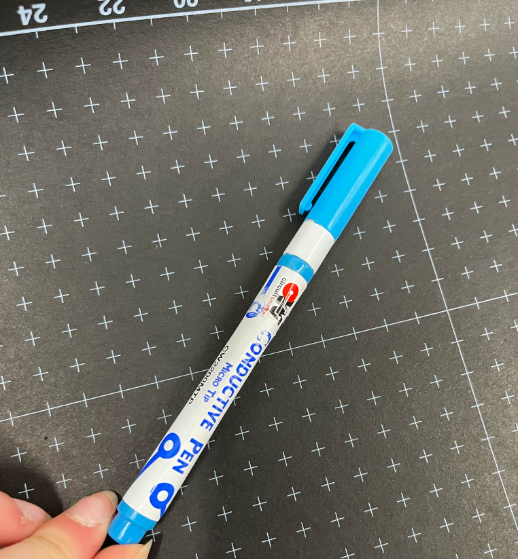
\includegraphics[width=\linewidth]{screenshot002}
		\caption{Paper conductor i retolador de tinta basada en una suspensió de plata.}
		\label{fig1.1a}
	\end{subfigure}
	\hfill
	\begin{subfigure}{0.45\textwidth}
		\centering
		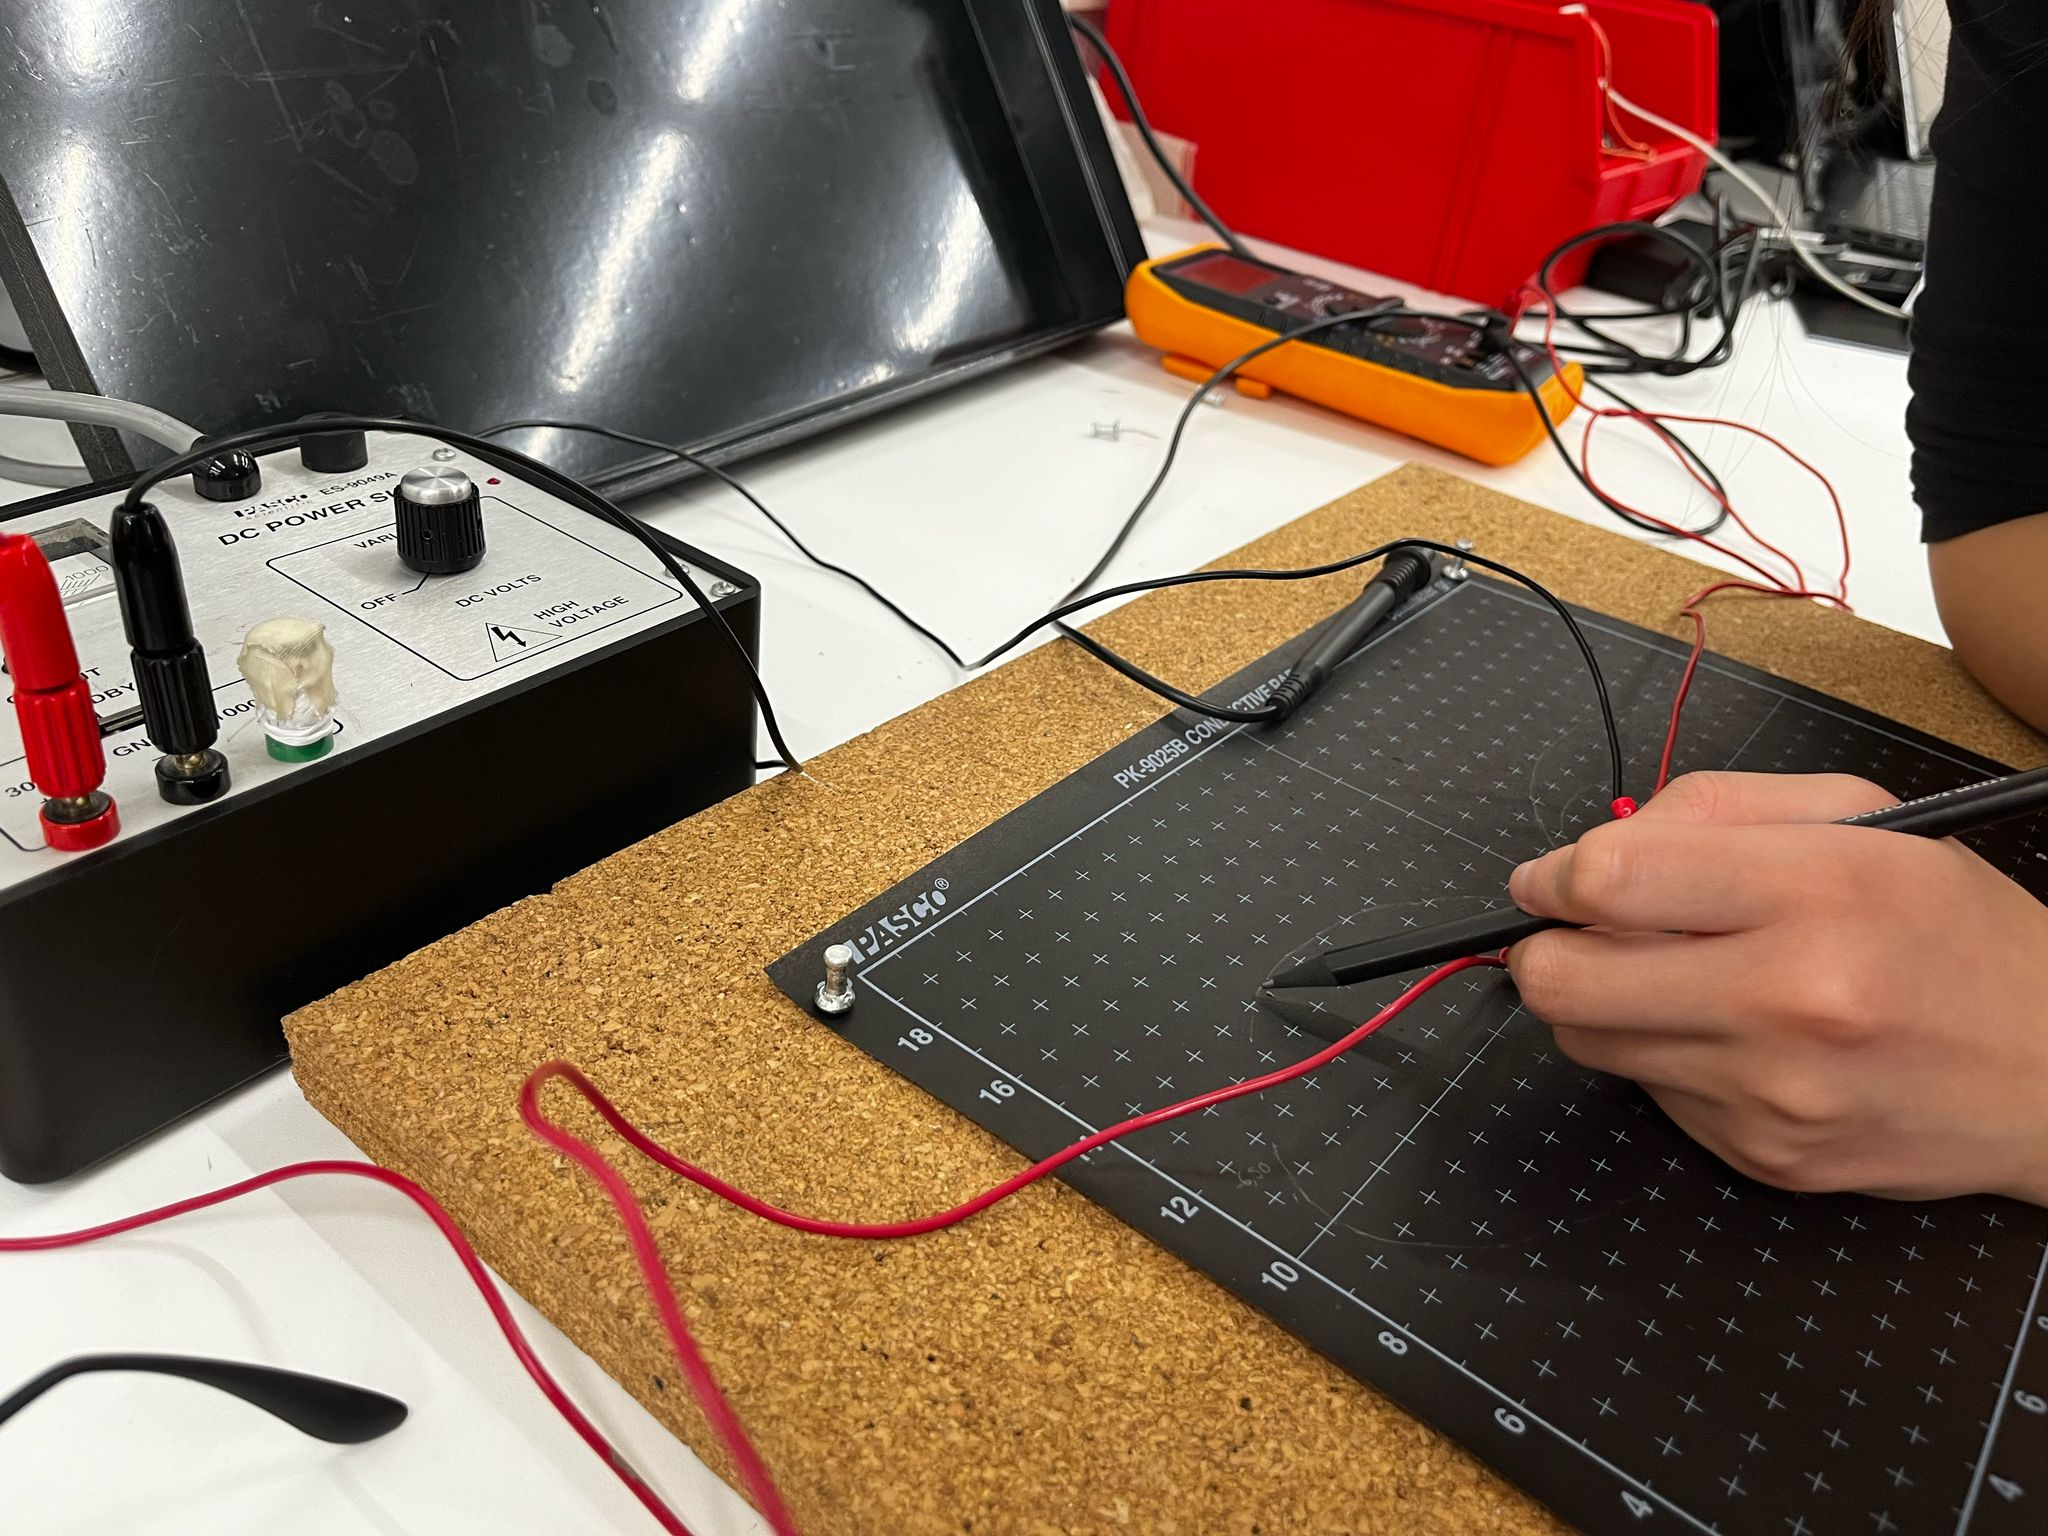
\includegraphics[width=\linewidth]{screenshot003}
		\caption{Muntatge experimental per a la representació de les corbes equipotencials pels dos fils infinits. D'esquerra a dreta: Font de corrent DC connectada als dos elèctrodes (dos punts pel cas representat) mitjançant dos cables; suro amb el paper conductor en el que prèviament s'han dibuixat els dos elèctrodes, enganxat amb xinxetes; multímetre usat per mesurar les diferències de potencial.}
		\label{fig1.1b}
	\end{subfigure}
	\caption{Paper conductor i muntatge experimental per a la representació de les corbes equipotencials.}
	\label{fig1.1}
\end{figure}

Hem treballat amb les següents tres distribucions: dues línies verticals (que són la projecció d'un condensador de plaques planoparal·leles), dos punts (projecció de dos fils infinits) i dues línies secants amb un punt entre elles (projecció de dos plans infinits formant angle d'aproximadament 60 º amb un fil infinit entre els dos).

Amb el pretext de generar el camp sobre les distribucions dibuixades, s'ha fixat el paper conductor (en el qual hem fet els dibuixos) sobre un suro usant xinxetes i hem connectat els elèctrodes (per a cada distribució per separat) a una font de corrent continu (DC) usant un parell de cables i més xinxetes. Per mesurar la diferència de potencial hem usat un multímetre, deixant un cable fixat a un dels dos elèctrodes (establint així una referència de potencial) i l'altre lliure per tal de fer mesures de $\Delta V$ a qualsevol altre punt del paper (veure figura \ref{fig1.1b}). Prèviament, però, ens hem assegurat què la diferència de potencial entre dos punts en els conductors (els elèctrodes dibuixats) no fos major de l'1\%\footnote{Recordem que, per ser aquests materials conductors, hem de tenir un potencial constant en tot el seu volum i, en particular, sobre la seva superfície.}.

Per dibuixar les corbes equipotencials usem el cable lliure del multímetre per buscar aquestes corbes sobre el paper. Marquem tots els punts que estan a un mateix potencial amb un llapis i, tot seguit, unim aquests punts amb una línia. Repetint això un seguit de cops podem construir vàries corbes equipotencials. Per tal d'assegurar-nos que es tanquen, és millor que comencem a buscar les corbes des de l'exterior dels nostres elèctrodes. Si comencem per l'interior, com que tindrem una densitat de corbes molt major, serà més fàcil que la línia escollida no s'acabi tancant. Veurem que ens interessa trobar corbes que tanquin els nostre elèctrodes per tal de poder aplicar el teorema de Gauss (en especial pel cas del condensador de plaques planoparal·leles).

Finalment, per representar el camp elèctric $\vec{E}$, hem dibuixat línies que sortien dels elèctrodes i tallaven les corbes equipotencials perpendicularment (en ambdós casos). 

\subsection{Càlcul de la capacitat del condensador}
Si aproximem la integral donada per l'equació \eqref{eq1.13} per un sumatori i calculem el camp $E_i$ segons
\begin{equation}
	E_i \approx \frac{\Delta V_i}{\Delta r_i} \label{eq1.14},
\end{equation}
on $\Delta r_i$ és la distància radial, $\Delta V_i$ és la diferència de potencial de l'element $\Delta l_i$, i el subíndex $i$ fa referència a la \textit{i-èssima} mesura. De tot això tenim:
\begin{equation}
	\frac{Q}{Z} \approx \varepsilon \sum_i \frac{\Delta V_i \Delta l_i}{\Delta r_i}.
\end{equation}
Usant que la capacitat d'un condensador de plaques planoparal·leles es correspon amb 
\begin{equation}
	C = \frac{Q}{\Delta V},
\end{equation}
la capacitat per unitat de longitud sota les aproximacions usades és:
\begin{equation}
	\frac{C}{Z} = \frac{Q/Z}{\Delta V} = \frac{\varepsilon}{\Delta V} \sum_i \frac{\Delta V_i \Delta l_i}{\Delta r_i} \label{eq1.17},
\end{equation}
on $\Delta V$ és la diferència de potencial a la qual hem sotmès les dues plaques del condensador.

\subsection{Distribució extra. Motivació}
Més enllà de les distribucions del condensador de plaques planoparal·leles i els dos fils infinits, treballem amb una tercera distribució: dos plans infinits secants (formant un angle de 60º) entre els quals tenim un fil infinit.

La raó per la qual hem decidit estudiar aquesta configuració és que ens servirà per comprovar si el mètode de les imatges és vàlid en aquest tipus de sistemes per tal de trobar la funció $\phi(\vec{r})$. El potencial generat per aquesta distribució es pot entendre com la superposició dels potencials creats per un conjunt de càrregues individuals distribuïdes adequadament (satisfent les mateixes condicions de contorn). En virtut del teorema d'unicitat, la solució de l'equació de Laplace de les dues distribucions és igual (llevat d'una constant), de forma que podem usar la darrera (més simple) per trobar el potencial de la primera (més complexa). 

A més a més, es pot demostrar fàcilment que en funció de l'angle d'intersecció entre els plans, la quantitat de càrregues imatge necessàries per reproduir el potencial del sistema variarà, satisfent que:
\begin{equation}
	N_q = \frac{360\text{º}}{\theta}-1 \label{eqimatges},
\end{equation}
on $N_q$ és el nombre de càrregues imatge i $\theta$ l'angle format pels dos plans. Fixem-nos en què $\theta = 180\text{º} \Rightarrow N_q = 1$, $\theta=90\text{º}\Rightarrow N_q =3$,$\dots$\footnote{Aquests són els resultats que vam veure en el problema 2.31 de la col·lecció de problemes de l'assignatura d'\textit{Electromagnetisme} (veure \cite{ref1}).} 
\subsection{Simulacions}
Els codis de les simulacions es poden trobar a l'annex \ref{an:a4}.

Per tal de simular el condensador planoparal·lel, considerem la distribució representada com la suma de doscentes càrregues puntuals (de valor $-q$ pel fil de l'esquerra i $q$ pel de la dreta) distribuïdes uniformement en les plaques, de manera que una es troba a $x = d/2$, i l'altra a $x = - d/2$. Pel que fa a l'eix de les ordenades, les càrregues estan situades des de $y = -H/2$ fins a $y = H/2$, on $H$ és l'alçada de la placa. Així, per a cada una de les càrregues, calculem la seva contribució al potencial i al camp elèctric en tots els punts de la malla $(X, Y)$ usant el principi de superposició.

Per la simulació dels dos fils infinits, considerem la seva projecció en el pla X$-$Y com dues càrregues puntuals separades una distància $d+2r$, essent aquest valor la separació entre els centres dels discos dibuixats experimentalment (de radi $r$).

Definim les funcions que descriuen el potencial i el camp elèctric corresponents a les expressions analítiques d'aquests magnituds per a una càrrega puntual. Així podem calcular la contribució de cada una en tots els punts de la malla aplicant el principi de superposició. D'aquesta manera obtenim el camp elèctric i el potencial total en cada punt de l’espai.

Per simular la tercera distribució de càrrega posem l'origen de coordenades en el punt on s'intersequen els plans i definim $d$ com la distancia en l'eix $x$ des de l'origen al fil infinit. A partir d'aquí, efectuem dues simulacions diferents:
\begin{itemize}
	\item En virtut del mètode de les imatges, podem substituir la nostra distribució per un conjunt de càrregues que satisfacin les condicions de contorn (potencial constant i igual a zero sobre els plans conductors); així doncs, simulem les corbes equipotencials i les línies de camp generades per cinc (veure equació \eqref{eqimatges}) càrregues imatge (i la real) a una distància $d$ de l'origen i separades entre elles 60º. Això és, però, assumint que els nostres plans són infinits.
	\item Per altra banda, simulem la nostra distribució per integració directa del potencial. Els detalls es poden trobar a l'annex \ref{an:a6}.
\end{itemize}

\section{Resultats i discussió}
Els resultats experimentals es poden trobar a l'annex \ref{an:a2}.

\subsection{Condensador de plaques planoparal·leles}
La primera configuració estudiada es correspon amb un condensador planoparal·lel, format per dos plans infinits (en l'eix Z, perpendicular al pla de la imatge) carregats i separats per una distància $d$. La seva projecció en el pla X$-$Y  resulta en dos fils infinits separats també per una distància $d$.

Les corbes equipotencials trobades experimentalment són les que es poden observar a la figura \ref{fig:1.2a}. Observem que dins la regió entre plaques, les línies equipotencials es mantenen gairebé paral·leles, indicant un camp elèctric gairebé uniforme i dirigit perpendicularment cap a les plaques. 

A les vores de les plaques, es manifesta l’efecte punta (degut a l'acumulació de càrregues a la superfície), on el camp deixa de ser uniforme i es distribueix de manera més complexa, amb línies equipotencials corbades cap a l’exterior. Aquest efecte és més acusat en condensadors de mida finita, ja que en el cas ideal de plaques infinites, el camp fora de la regió entre elles seria nul. Els resultats són, aproximadament els mateixos predits per la simulació de la figura \ref{fig:1.2b}.

Com ja hem comentat abans, podem utilitzar la llei de Gauss per tal de calcular la capacitat per unitat de longitud que tindria el condensador infinitament llarg en la direcció $Z$. Per fer-ho emprem l'expressió \eqref{eq1.17}, prèviament deduïda, i els resultats experimentals obtinguts en el transcurs de la pràctica\footnote{Aquests es poden trobar a la taula de l'annex \ref{an:a2}.}:
\begin{equation}
	\frac{C}{Z} = \frac{Q/Z}{\Delta V} = \frac{\varepsilon}{\Delta V} \sum_i \frac{\Delta V_i \Delta l_i}{\Delta r_i} = (2,06 \pm 0,21)\varepsilon \text{ F/m}.
\end{equation}
Podem comparar aquest resultat amb el que s'obtindria si tinguéssim un condensador ideal de plaques planoparal·leles si usem que\footnote{Les mesures per $H$ i $d$ s'han efectuat digitalment amb \textit{ImageJ}.}:
\begin{equation*}
	H = (7,961\pm0,001) \text{ cm}, \hspace{0.25cm} d = (5,598\pm0,001) \text{ cm}.
\end{equation*}
De manera que:
\begin{equation}
	\frac{C}{Z} = \frac{A\varepsilon/d}{Z} = \frac{H}{d}\varepsilon = (1,4221 \pm 0,0003)\varepsilon \text{ F/m},
\end{equation}
on $A$ es l'àrea de la placa i $H$ l'altura d'aquesta. 
Veiem que el nostre condensador es desvia notablement del cas ideal. És més, segons els nostres càlculs, el condensador real té una capacitat per unitat de longitud superior, cosa que, a priori, no pot ser. 

Hi ha principalment dos motius pels quals no hem obtingut la càrrega per unitat de longitud real: Primer, experimentalment hauríem d'haver fet més punts per tal tenir unes línies de camp més precises i així poder fer una millor aproximació a la integral donada per \eqref{eq1.17}; segon, i més important, perquè aquesta aproximació sigui lo més bona possible, cal que la suposició donada per l'equació \eqref{eq1.14} sigui també molt bona, i per tal que això sigui així, cal que les línies equipotencials mesurades experimentalment siguin molt properes, ja que, per poder assegurar que
\begin{equation}
	E = \frac{\partial V_i}{\partial r_i} \approx \frac{\Delta V_i}{\Delta r_i},
\end{equation}
és necessari que el $\Delta r_i$ entre les corbes equipotencials sigui suficientment petit com per que $\Delta r_i \rightarrow \partial r_i$ i que, a més a més, estigui en al direcció perpendicular a les corbes equipotencials, per tal de poder dir que la suposició donada a \eqref{eq1.14} és vàlida. En el nostre cas, òbviament això no és estrictament correcte, ja que la separació entre les línies equipotencials no és negligible i el $\Delta r_i$ no necessàriament és perpendicular a aquestes. 

\begin{figure}
	\centering
	\begin{subfigure}{0.45\linewidth}
		\centering
		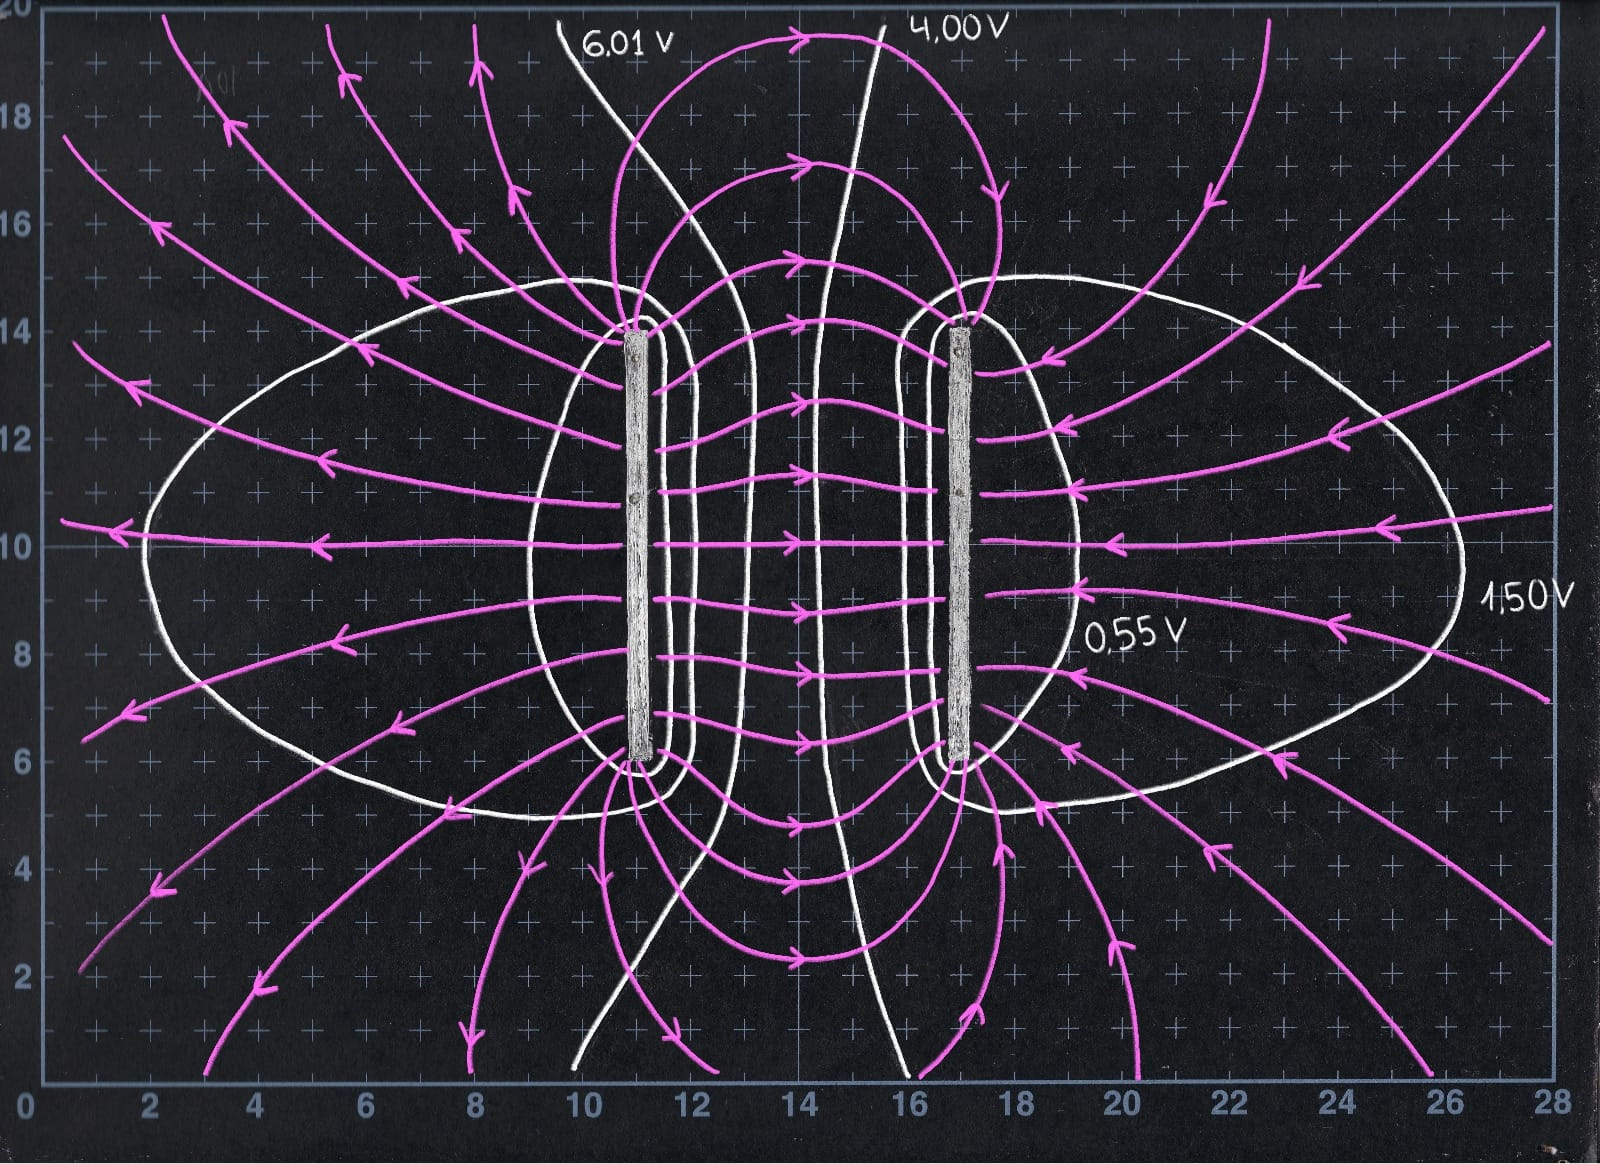
\includegraphics[height=5.5cm]{dibplaques} % Augmenta la mida
		\caption{Corbes equipotencials (en blanc) i línies de camp $\vec{E}$ (en lila) pel cas del condensador planoparal·lel trobades experimentalment.}
		\label{fig:1.2a}
	\end{subfigure}
	\hfill
	\begin{subfigure}{0.53\linewidth}
		\centering
		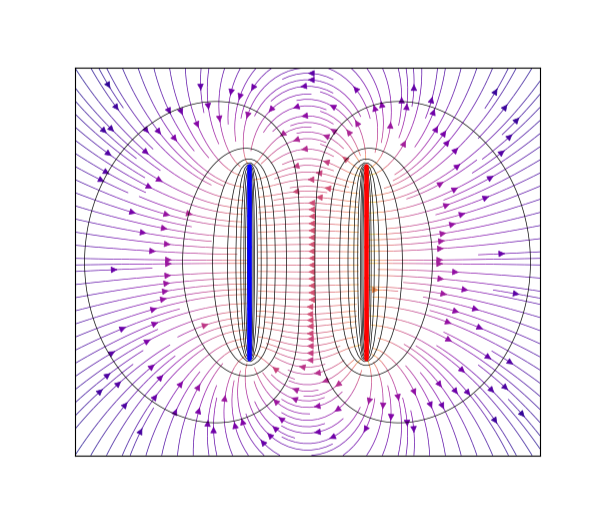
\includegraphics[height=6.5cm]{figplaques1} % Mateixa alçada
		\caption{Simulació del camp elèctric i del potencial pel condensador planoparal·lel.}
		\label{fig:1.2b}
	\end{subfigure}
	\caption{Representació i simulació de les corbes equipotencials i línies de camp per la distribució associada al condensador planoparal·lel.}
	\label{fig:1.2}
\end{figure}

Fixem-nos en què, a més a més, en el cas del condensador planoparal·lel, la relació entre $H$ i $d$ satisfà que $d/H \rightarrow 0$ (la separació entre les dues plaques és molt més petita que les dimensions característiques d'aquestes). En el nostre cas, però, això no és així; si ens atenim a les mesures de $H$ i $d$ ràpidament veiem que $H\approx d$ (són del mateix ordre!), de forma que $d/H\neq 0$ i l'anterior condició no se satisfà. Aquest és un motiu més pel qual no s'ha obtingut la càrrega per unitat de longitud real.
\subsection{Fils infinits}
La segona configuració estudiada és la projecció en el pla X$-$Y (pla de la imatge) de dos fils infinits separats per una distància constant. 

Les corbes equipotencials trobades experimentalment són les que es poden observar a la figura \ref{fig:1.3a}. Observem com aquestes formen el·lipses on els fils estan cada cop més descentrats conforme agafem corbes més externes. 
\begin{figure}[h]
	\centering
	\begin{subfigure}{0.45\linewidth}
		\centering
		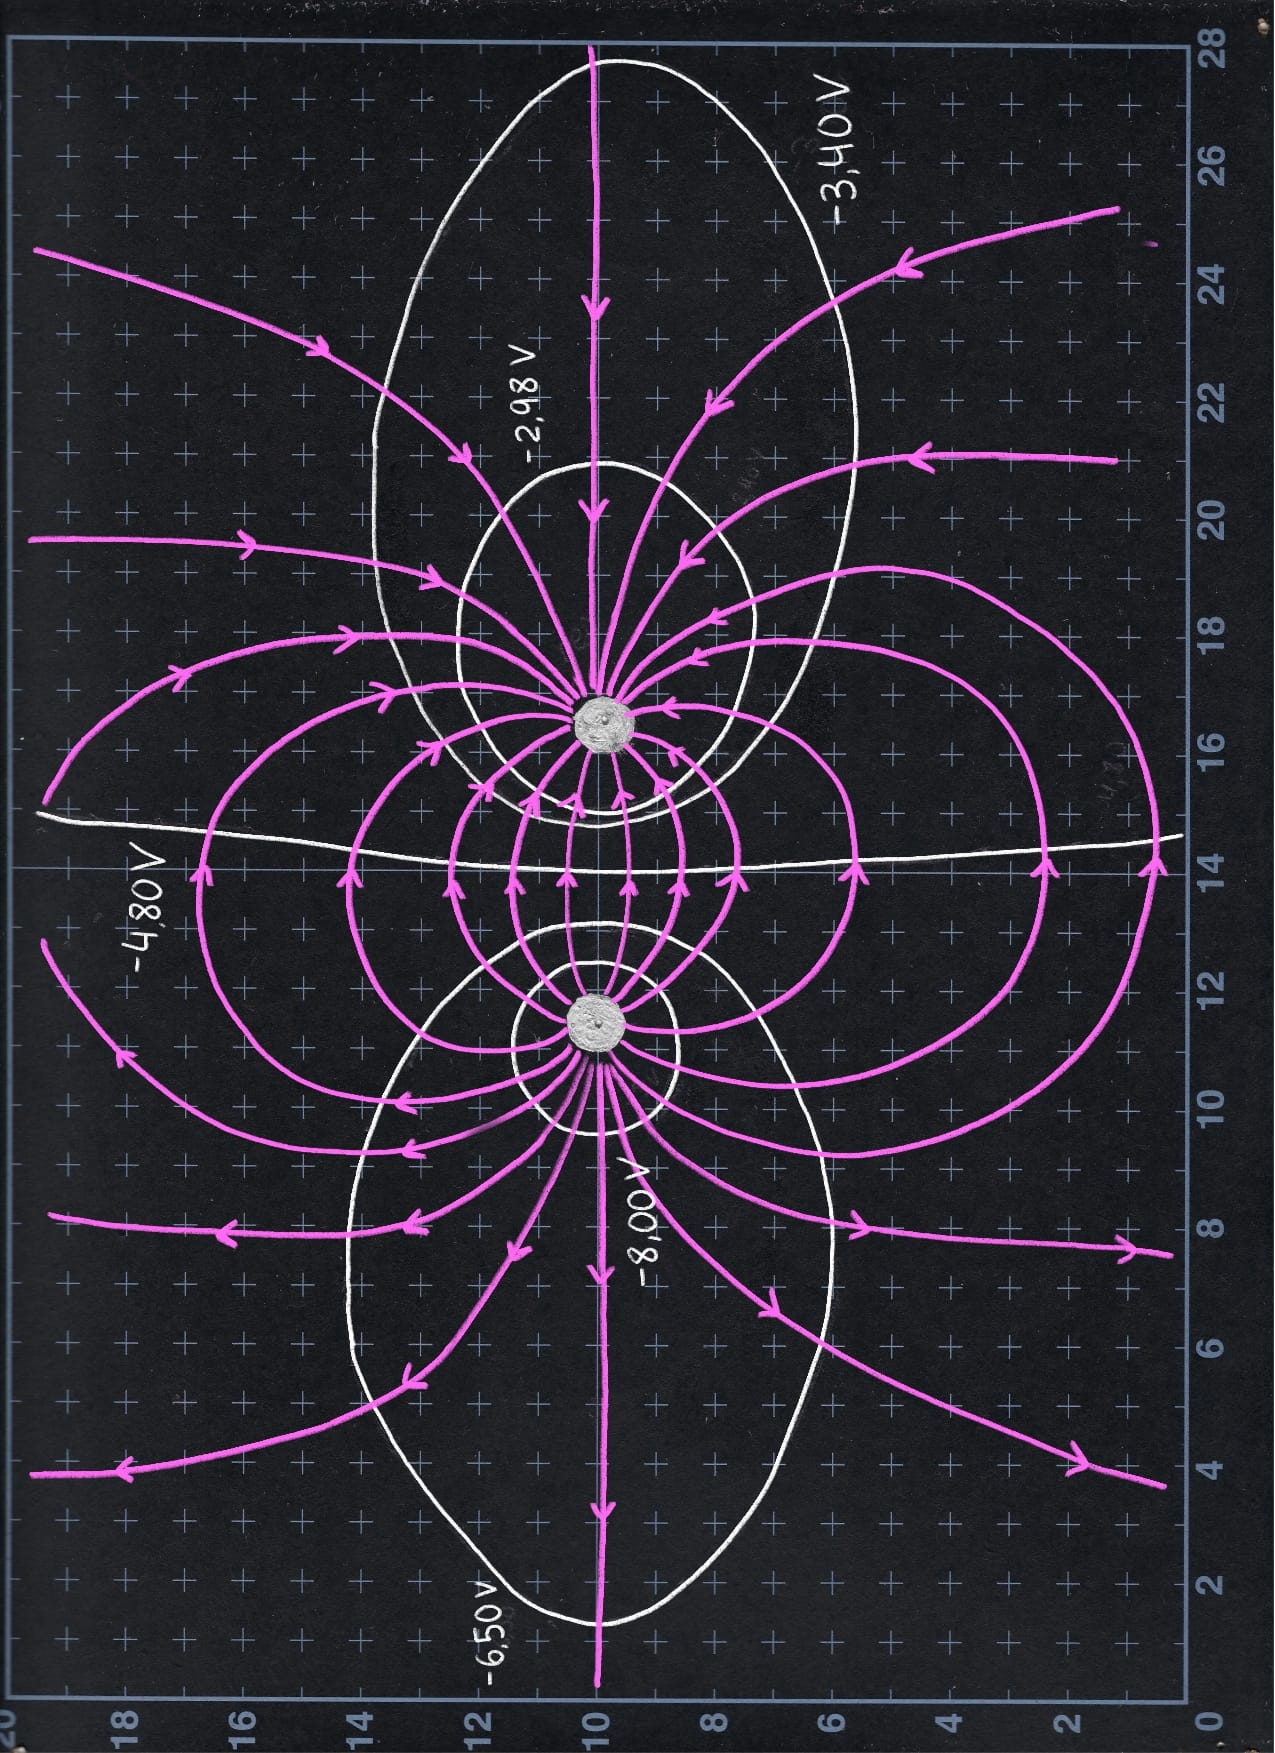
\includegraphics[angle=270,width=\linewidth]{screenshot004}
		\caption{Corbes equipotencials (en blanc) i línies de camp $\vec{E}$ (en lila) pel cas dels dos fils infinits trobades experimentalment.}
		\label{fig:1.3a}
	\end{subfigure}
	\hfill
	\begin{subfigure}{0.5\linewidth}
		\centering
		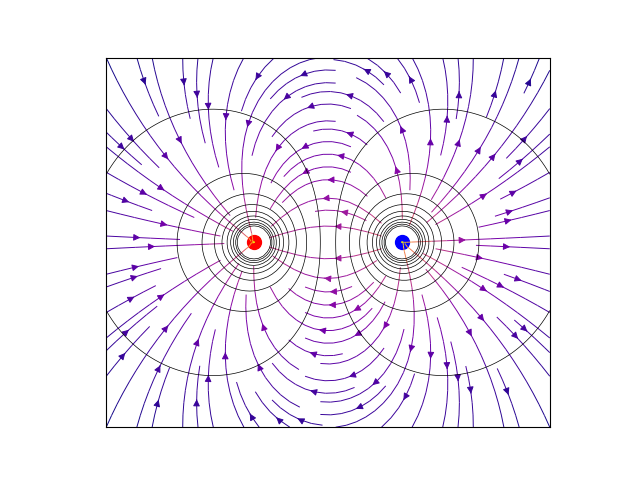
\includegraphics[width=\linewidth]{figfils}
		\caption{Simulació del camp elèctric i del potencial pels dos fils infinits.}
		\label{fig:1.3b}
	\end{subfigure}
	\caption{Representació i simulació de les corbes equipotencials i línies de camp per la distribució de dos fils infinits.}
	\label{fig:1.3}
\end{figure}

Els resultats teòrics indiquen que, en un sistema de dos fils infinits, les corbes equipotencials venen donades per la següent equació:
\begin{equation}
	y^2+\left( x+a\frac{1+k^2}{1-k^2}\right)^2 = a^2\left( \frac{2k}{1-k^2}\right)^2  \label{eqsuppon},
\end{equation}
que és l'equació d'una circumferència. Per tant, les corbes equipotencials teòriques haurien de ser circumferències de radi $R = a\frac{2k}{1-k^2}$ amb el centre lleugerament desplaçat en l'eix de les $x$ per un factor $a\frac{1+k^2}{1-k^2}$. Notem que tant $a$ com $k$ són dues constants\footnote{Els valors de les constants i la demostració d'aquest resultat es pot trobar a l'annex \ref{an:a1}.}. Es pot veure que es compleix exactament el que s'ha descrit atenint-nos als resultats obtinguts a la simulació de la figura \ref{fig:1.3b}.

El fet que els nostres resultats es desviïn del predit per la teoria es deu als diferents errors experimentals comesos durant l'evolució de la pràctica. Els principals factors que poden alterar els resultats de l'experiment són: s'assumeix que el paper conductor té una conductivitat $\sigma$ homogènia, però això no necessàriament ha de ser així (pot ser que presenti inhomogeneïtats), els punts que representen la projecció dels dos fils infinits en el pla no són perfectament rodons, ja que han sigut dibuixats a mà (amb les imprecisions que això comporta). Pel que fa a les corbes equipotencials i les línies de camp, aquestes es poden veure afectades per l'efecte punta a les vores dels materials carregats, on s'acumula més densitat de càrrega. 

A tots aquests efectes cal sumar dos fenòmens més: El paper conductor és finit, cosa que afecta a les condicions de contorn del sistema (no podem situar l'origen de potencial a l'infinit) i, a més a més, els dos suposats fils infinits no són fils, són cilindres que no necessàriament tenen el mateix radi. Tot plegat podria explicar les desviacions observades.

\subsection{Fil infinit i dos plans}

La tercera configuració estudiada i proposada per nosaltres és la projecció en el pla X$-$Y de dos plans infinits (en l'eix $Z$) formant un angle de $60^o$ amb més un fil infinit (en l'eix $Z$) situat dins de la regió entre els plans.

Les corbes equipotencials trobades experimentalment són les que es poden observar a la figura \ref{fig:1.4a}.

\begin{figure}[h]
	\centering
	\begin{subfigure}{0.49\linewidth}
		\centering
		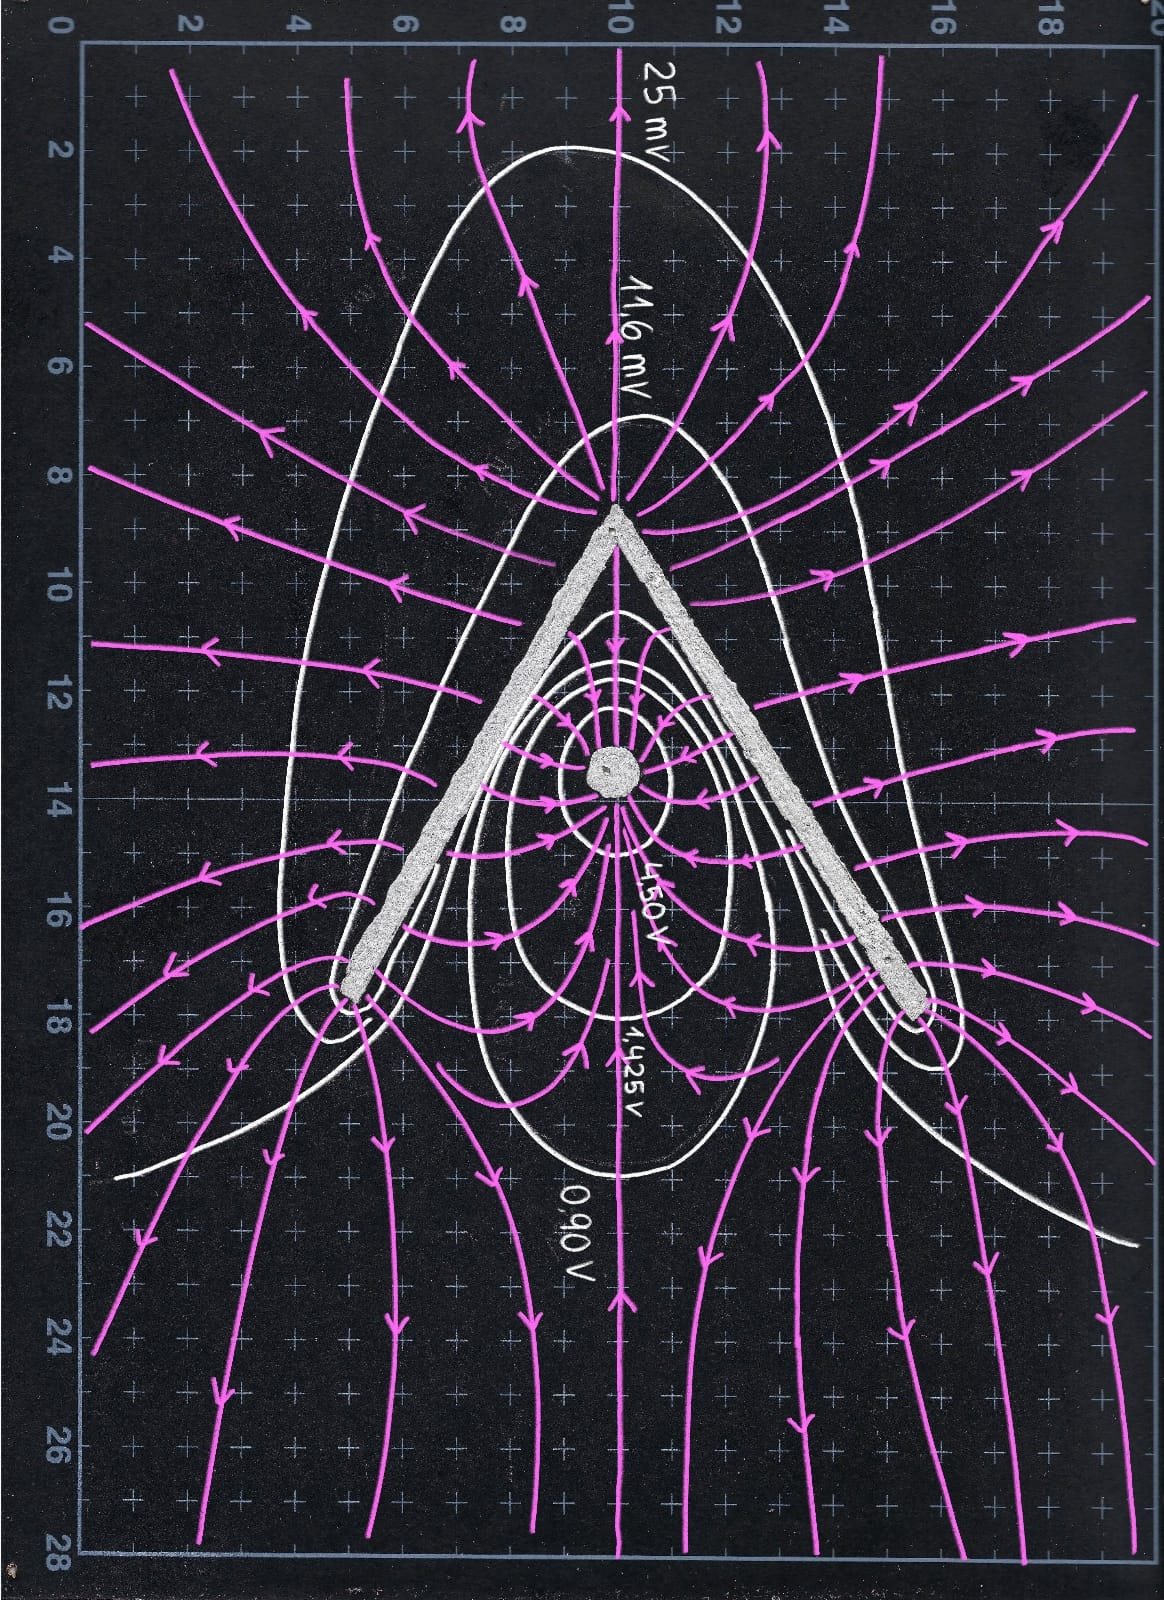
\includegraphics[angle=90, width=\linewidth]{confinventJS}
		\caption{Corbes equipotencials (en blanc) i línies de camp $\vec{E}$ (en lila) pel cas dels dos plans infinits i un fil infinit trobades experimentalment.}
		\label{fig:1.4a}
	\end{subfigure}
	\hfill
	\begin{subfigure}{0.49\linewidth}
		\centering
		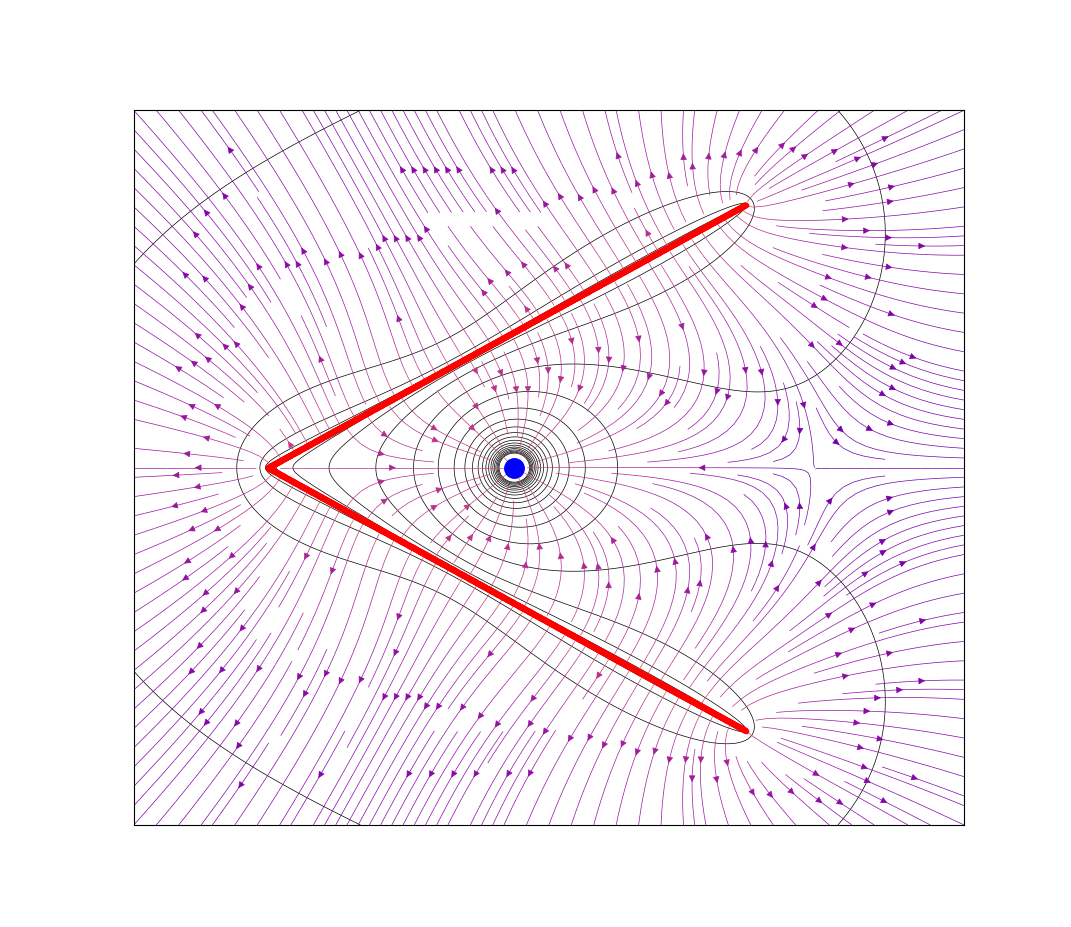
\includegraphics[width=\linewidth]{figplacarara}
		\caption{Simulació del camp elèctric i del potencial pels dos plans i el fil infinit.}
		\label{fig:1.4b}
	\end{subfigure}
	\caption{Representació i simulació de les corbes equipotencials i línies de camp per la distribució de dos plans infinits amb un fil infinit enmig.}
	\label{fig:1.4}
\end{figure}

Notem que aquesta configuració de càrrega és molt més complexa que les anteriors, ja que una de les distribucions, pel fet de ser triangular, l'efecte punta es fa molt notable als extrems. De fet, veiem que en aquests punts el camp divergeix molt més que en altres regions.

\begin{figure}[h]
	\centering
	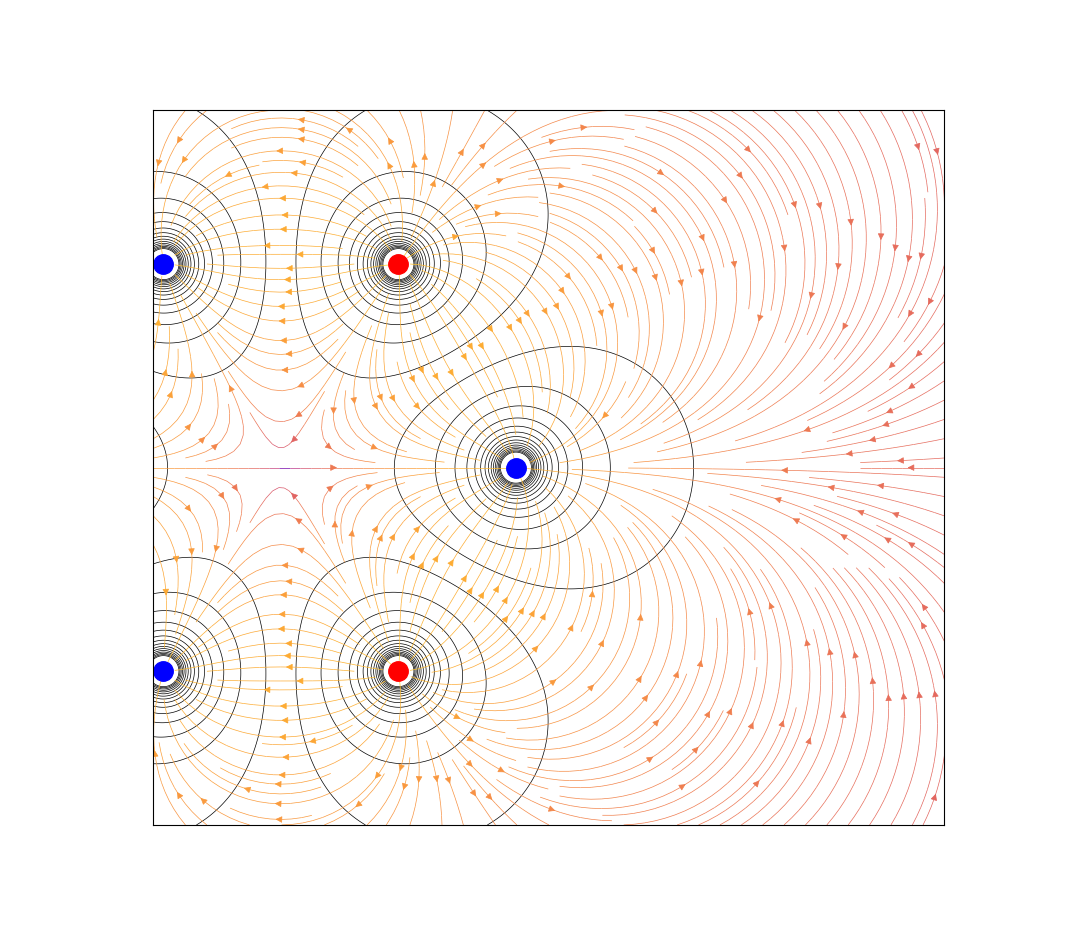
\includegraphics[width=0.45\linewidth]{figV2imagenes}
	\caption{Simulació de les corbes equipotencials i de les línies de camp elèctric associades a la distribució de càrregues imatge solució.}
	\label{fig:1.5}
\end{figure}

Hem fet la simulació pel mètode de les imatges que presentem a la figura \ref{fig:1.5}. Aquesta presenta un comportament molt similar a l'obtingut experimentalment. Pel que fa a la regió entre la càrrega i les plaques, els resultats són pràcticament idèntics, però conforme ens allunyem de la càrrega, el comportament comença a diferir. Podem trobar un clar exemple fixant-nos en punts situats sobre l'eix de les abscisses amb un valor de $x$ gran. En aquesta regió, tant en la representació experimental com en l'analítica, el camp apunta cap a fora de la distribució, metre que en la simulació pel mètode de les imatges és al revés.

Les diferències esmentades posen de manifest que la solució trobada a partir del mètode de les imatges no pot ser comparada a determinades regions de l'espai, principalment perquè aquesta solució considera les plaques infinites (i clarament les nostres no ho són). Per tant, la comparació amb els  resultats experimentals només té sentit si ens trobem dins del món real però mantenint-nos a les proximitats del fil.


\section{Conclusions}
Aquesta pràctica s'ha basat en l'ús d'un multímetre per tal de mesurar el potencial elèctric a diferents distàncies de les distribucions de càrrega dibuixades. Això ens ha permès, per una banda, traçar línies equipotencials i, per altra, obtenir un valor de la capacitat per unitat de longitud d'un condensador.

Hem pogut veure com les línies equipotencials dibuixades es corresponien força bé amb les prediccions teòriques, que ens diuen que, a les proximitats de la superfície dels conductors, aquestes línies són tangents al conductor. A més a més, ens han servit de guia per dibuixar, posteriorment, les respectives línies de camp elèctric, ja que, com sabem de teoria, aquestes són perpendiculars a les equipotencials. Tanmateix, per a les tres geometries considerades, hem generat les corresponents simulacions basades en mètodes numèrics èr tal de poder comparar els resultats experimentals amb els teòrics amb més facilitat.

Addicionalment, per a la tercera distribució (dos plans secants i un fil infinit), com que coneixíem la solució que ens dona el mètode de les imatges (motiu pel qual l'hem escollit), hem pogut contrastar les línies equipotencials i de camp trobades experimentalment amb les del mètode mencionat, verificant així la validesa d'aquesta solució.

Tal i com s'ha anat comentant, tant les línies equipotencials com les de camp basades en les mesures del multímetre (resultats experimentals) segueixen la mateixa tendència que les simulacions. Tot i no coincidir-hi exactament a causa dels diferents problemes ja discutits (efecte punta, inhomogeneïtats del paper, haver dibuixat formes irregulars, imprecisions causades pel gruix de la punta del llapis, paper conductor finit, ...), la geometria i el sentit de les línies de camp són coherents.

Per altra banda, hem calculat la capacitat per unitat de longitud d'un condensador de plaques planoparal·leles a partir del teorema de Gauss. Com s'ha explicat, el càlcul experimental s'ha realitzat amb un sumatori com a aproximació de la integral de l'equació \ref{eq1.13}. Atès que el resultat obtingut és coherent amb el valor teòric esperat, podem considerar vàlida l'aproximació emprada.

Així, a partir de tres distribucions de conductors diferents amb suficient simetria com per reduir el problema a dues dimensions, hem comprovat l'existència de la dualitat entre la densitat de corrent $\vec{J}$ i el vector desplaçament $\vec{D}$.

\chapter{Força entre corrents}
\begin{chapterabstract}
	En aquesta pràctica mesurem la força entre dos fils pels quals hi circula un corrent elèctric, comprovant que la llei de Biot i Savart se satisfà, via diferents metodologies. Amb aquests resultats fem una estimació de la permeabilitat magnètica al buit $\mu_0$, tot comparant-la amb el valor teòric. A més a més, utilitzant el mateix sistema, mesurem la component horitzontal del camp magnètic terrestre al laboratori.
\end{chapterabstract}
\section{Introducció i fonament teòric}
Per quantificar la interacció magnètica entre dos circuits arbitraris tancats pels quals hi circula un corrent constant, és a dir, per mesurar la força que fa un circuit sobre l'altre podem usar que
\begin{equation}
	\vec{F}_1 = \frac{\mu_0}{4\pi}I_1I_2\oint \oint \frac{\mathrm{d}\vec{l}_1\cross[\mathrm{d}\vec{l}_2 \cross (\vec{r}_1-\vec{r}_2)]}{\abs{\vec{r}_1 - \vec{r}_2}^3}\label{eq:2.1},
\end{equation}
on $I_1$ i $I_2$ són les intensitats dels circuits 1 i 2, respectivament, d$\vec{l}_1$ i d$\vec{l}_2$ són els elements infinitesimals de línia i $\vec{r}_1$ i $\vec{r}_2$ són les respectives posicions d'aquests elements.

Per tal de simplificar la integral anterior definim el camp d'inducció magnètica (o densitat de flux magnètic) $\vec{B}(\vec{r})$ en un punt arbitrari $\vec{r}$ com
\begin{equation}
	\vec{B}(\vec{r}) = \frac{\mu_0}{4\pi} \int_V \vec{J}(\vec{r}_1)\cross\frac{\vec{r}-\vec{r}'}{\abs{\vec{r}-\vec{r}'}^3}\mathrm{d}^3r'.
\end{equation} 
Si usem això sobre l'equació \eqref{eq:2.1} podem escriure la força que rep el circuit amb intensitat I degut a la presència del camp d'inducció $\vec{B}$ creat per l'altre circuit segons
\begin{equation}
	\vec{F} = I \oint \mathrm{d}\vec{l}\cross\vec{B}(\vec{r}). \label{eq2:3}
\end{equation}
Emprant una de les equacions pel camp $\vec{B}$
\begin{equation}
	\vec{\nabla}\cross \vec{B} = \mu_0 \vec{J},
\end{equation}
i aplicant el teorema de Stokes
\begin{equation}
	\oint_C \vec{A} \cdot \mathrm{d}\vec{r} = \int_S (\vec{\nabla}\cross \vec{A})\cdot \mathrm{d}\vec{S},
\end{equation}
podem deduir fàcilment el teorema d'Ampère, que ens diu que:
\begin{equation}
	\oint_C\vec{B}\cdot\mathrm{d}\vec{l} = \mu_0\int_S\vec{J}(\vec{r})\cdot\vec{n}\mathrm{d}S,
	\label{eq2:6}
\end{equation}
d'on, via un càlcul ràpid, podem trobar el camp d'inducció magnètica generat per un fil infinit amb intensitat $I$ a una distància $r$ del seu centre
\begin{equation}
	B = \frac{\mu_0 I}{2\pi r}. \label{eq2:7}
\end{equation}
Així doncs, la força, en mòdul, que patirà un altre fil paral·lel, de longitud $L$  i pel qual hi circula la mateixa intensitat $I$ serà
\begin{equation}
	F = \frac{\mu_0 I^2L}{2\pi r}, \label{eq2:8}
\end{equation} 
o, en termes de $B$
\begin{equation}
	F = BLI. \label{eq:2.campmagnetic}
\end{equation}
Aquesta darrera equació ens permetrà calcular el camp d'inducció magnètica terrestre\footnote{Nota: Ens referirem a $B$ de forma indistinta per \textit{camp magnètic terrestre} i \textit{camp d'inducció magnètica terrestre}.} (en particular la component horitzontal) a partir de la força que fa aquest sobre un fil de longitud $L$ pel qual hi travessa una intensitat $I$.
\section{Metodologia experimental}

El sistema que usarem per tal de fer totes les mesures necessàries serà el de la figura \ref{fig:2.1}\footnote{Tots els esquemes dels muntatges experimentals han estat extrets dels \textit{Guions de les pràctiques de l'assignatura de Laboratori d'Electromagnetisme}\cite{ref3}}. A l'esquema es poden veure tots els elements clau que constitueixen la balança usada. També usem una font de corrent continu, un transformador, un conjunt de masses (de 5, 10, 15 i 25 mg) i una brúixola.

\begin{figure}[h]
	\centering
	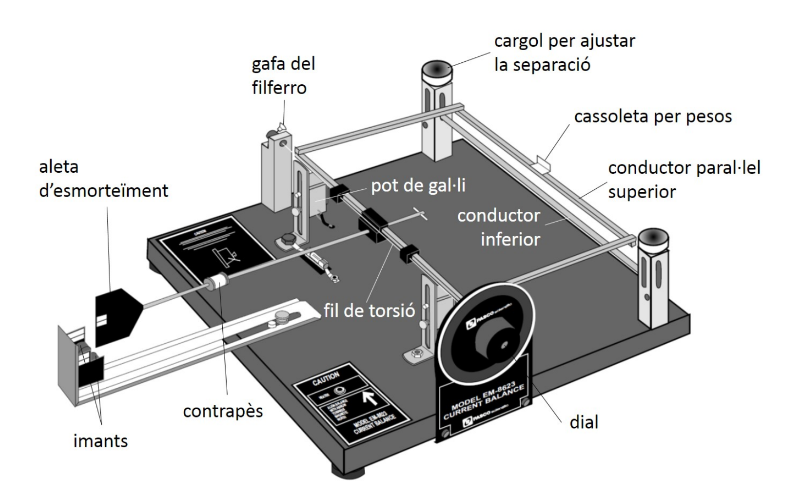
\includegraphics[width=0.6\linewidth]{screenshot008}
	\caption{Esquema de la balança usada en el transcurs de la pràctica 2.}
	\label{fig:2.1}
\end{figure}

Abans de començar amb l'equilibrat de la balança connectem el transformador a 9 V (al lloc indicat amb 'HEATER 9 V') per tal de fondre el gal·li ($T \approx 30$ ºC), que actuarà com a conductor. Tot seguit orientem la balança de forma que els dos fils conductors estiguin en la direcció nord-sud; així evitem els possibles efectes causats pel camp magnètic terrestre. Seguidament connectem la font de corrent continu, tal i com es pot veure a la figura \ref{fig:2.2}, tot assegurant-nos que està en 'OFF' i que els controls d'intensitat i de potencial estan al mínim i al màxim, respectivament. Mesurem la longitud $L$ del fil.

\begin{figure}[h]
	\centering
	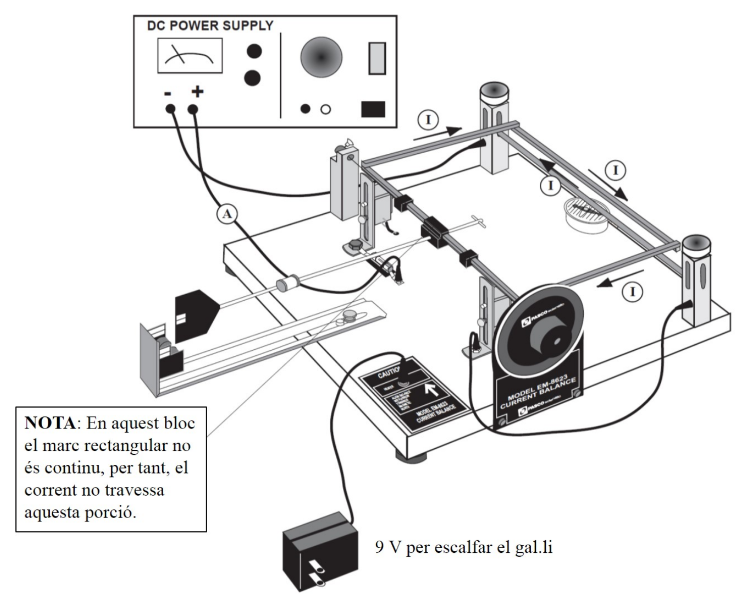
\includegraphics[width=0.6\linewidth]{screenshot009}
	\caption{Esquema de les connexions de la balança.}
	\label{fig:2.2}
\end{figure}

\subsection{Equilibrat de la balança}
Un cop tenim la balança preparada, cal que l'equilibrem. Primer fem baixar el pot de gal·li per fondre'l i, un cop és líquid, el tornem a pujar fins que toqui el conductor, sense que el darrer estigui totalment submergit. Repetim tot això per l'altre pot de gal·li. Posem el dial a zero i la gafa del filferro oposada a aquest, en posició vertical.

Tot seguit desplacem el contrapés fins que la balança està més o menys equilibrada. Seguidament ens assegurem d'ajustar bé el zero, fent que les dues ratlles de l'imant esmorteïdor i les de la paleta d'esmorteïment estiguin totalment alineades.

Finalment, usant els dos cargols per ajustar la separació entre fils, fem pujar el conductor inferior fins que toca en el màxim nombre de punts el conductor superior\footnote{Notem que, com que ambdós fils no són rectes, en cap moment poden tocar-se en \textit{tots} els punts.}, assegurant-nos que el zero de l'aleta no s'ha mogut (si ho fa, vol dir que els dos conductors estan fent força entre ells). Prenem nota de la posició del zero cargol; aquest es correspon a una separació de 3.1 mm entre els conductors (suma de radis o diàmetre).

\subsection{Força vs. corrent}
Per tal de mesurar la força entre els fils vs. corrent comencem baixant el conductor paral·lel inferior uns 5 mm (tenint present que cada volta dels cargols equival a 1 mm). Amb això ens assegurem que la separació entre els centres dels fils és de 8.1 mm. Seguidament posem una massa de 5 mg a la cassoleta de pesos i connectem la font de potencial. Ajustem el corrent continu fins que la balança torna al valor d'equilibri, tot prenent nota del valor de $I$. Desconnectem la font de potencial i agafem la massa de 5 mg; ens assegurem de que la balança, en absència de pesos i corrent, segueix al zero (en cas que no sigui així, cal repetir tot el procediment d'equilibrat de la balança).

Repetim tot això uns quants cops (tres en el nostre cas) per la massa de 5 mg i calculem el promig d'intensitats (així minimitzem els possibles errors experimentals que es puguin cometre).

Repetim els anteriors passos augmentant la massa de 5 en 5 mg fins a arribar a 25 mg (com a màxim) o fins que no puguem reequilibrar la balança.

Amb tot el recull de mesures d'intensitat representem $I^2$ vs. $F$ (massa $\cross$ gravetat)
\begin{equation}
	I^2 = \frac{2\pi r}{\mu_0 L} F. \label{eq:2.9}
\end{equation}
De l'anterior recta, a partir del pendent deduïm el valor de $\mu_0$. Recordem que $L$ és la longitud dels fils i $r$ la separació entre aquests.

\subsection{Força vs. separació}
Per tal de poder calcular un valor de $\mu_0$ experimental a partir de la força vs. separació, primer trobem la constant de torsió del fil, la qual relaciona la força del fil d'acer en funció de l'angle de torsió. Aquest paràmetre es pot obtenir equilibrant la balança (veure figura \ref{fig:2.1}) per a cada una de les masses (5, 10, 15, 20 i 25 mg) i anotant-ne els graus que cal girar el dial de la balança per tal d'equilibrar el pes d'aquestes. Comencem amb la massa de 20 mg a la cassoleta i després repetim el procediment amb la resta. Un cop tenim totes les dades, representem la gràfica de la força en funció de l'angle de torsió, trobant així el pendent de la recta 
\begin{equation}
	F=k\theta.
	\label{eq2:10}
\end{equation}
Notem que hem assumit que l'angle de torsió $\theta$ i la força $F$ són proporcionals, mitjançant una constant recuperadora $k$. Això que té sentit si pensem en la llei de Hooke, que, recordem, ens diu que la força recuperadora que fa una molla és
\begin{equation}
	F = k\Delta x,
\end{equation} 
on $k$ és la constant recuperadora de la molla i $\Delta x$ el desplaçament respecte de la posició d'equilibri de la darrera.

Seguidament es fixa un corrent d'entre 5 i 6 A que es mantindrà constant durant tot l'experiment. Comprovem que l'aparell continua equilibrat, ja que en cas contrari caldria repetir el procediment descrit a la Sec. 2.2.1. Ara, amb els cargols d'ajust de la balança, fixem també una separació $r$ màxima entre conductors. Aquesta distància serà la que anirem reduint per a cada mesura.

Així, comencem a una $r \sim$ 10 mm. Com que cada variació d'aquesta distància comporta un desequilibri de la balança, caldrà equilibrar-la de nou girant el dial uns determinats graus. D'aquesta manera obtenim les dades experimentals dels graus que es corresponen a cada separació fins una $r \sim$ 4mm. 

Un cop tenim aquestes mesures, només cal representar la força (calculada amb l'equació \eqref{eq2:10}) en funció de $1/r$, usant l'equació \eqref{eq:2.9}, de manera que
\begin{equation}
	k\theta = \frac{\mu_0LI^2}{2\pi}\frac{1}{r}. \label{eq:2.13}
\end{equation}
De la darrera equació, podem trobar el pendent a partir de la representació de $k\theta$ vs. $\frac{1}{r}$ i, amb aquest, el valor de $\mu_0$.
\subsection{Mesura del camp magnètic terrestre}
En aquest últim apartat, hem de canviar l'orientació de la balança per tal d'assegurar-nos que el camp d'inducció magnètica $\vec{B}$ de la Terra faci força sobre els fils; per fer-ho orientem els conductors de manera que la intensitat que els travessa quedi perpendicular a la direcció nord-sud de la Terra. Això s'aconsegueix fàcilment fent ús de la brúixola proporcionada.

Un cop ens hem assegurat que la balança continua equilibrada (en cas contrari caldria repetir el procediment descrit a la Sec. 2.1.1) es connecta la font d'alimentació de tal manera que només hi hagi intensitat en el conductor paral·lel superior.

Comencem l'experiment donant una intensitat d'uns 6 A i mesurant la força amb la metodologia seguida a la Sec. 2.2.3, és a dir, fent girar el dial fins equilibrar la balança i anotant-ne els graus necessaris. Cal fer vàries mesures amb diferents valors d'intensitats (menors als 6 A inicials), de manera que, fent una mitjana, podem extreure un valor experimental de la component horitzontal del camp magnètic de la Terra fent ús de l'equació \eqref{eq:2.campmagnetic}.

\section{Resultats i discussió}

\subsection{Valor experimental de la permeabilitat magnètica}
El càlcul de la permeabilitat magnètica del buit el fem a partir de les mesures de \textit{força vs. corrent} i de les mesures de \textit{força vs. separació}. 

De les mesures de $I^2$ vs. $F$, a partir de l'equació \eqref{eq:2.9}, trobem, després de fer un ajust lineal, la recta de la figura \ref{fig:2.3}\footnote{Totes les gràfiques s'han fet usant el programari \textit{Gnuplot}.}. Per arribar a aquests resultats fem tres mesures de la força per cada massa, per cinc masses diferents (les indicades a la secció del procediment experimental de la pràctica). Les dades experimentals usades es poden trobar en forma de taula a l'annex \ref{an:c1}. De l'ajust lineal de la figura \ref{fig:2.3} en determinem la permeabilitat magnètica del buit, ja que està directament relacionada amb el pendent d'aquesta recta, tenint present que els valors de la longitud del fil $L$, la separació entre fils $r$ i $g$ són
\begin{equation*}
	L = (0,305\pm 0,001)\text{ m}, \hspace{0.15cm} r = (8,10\pm 0,05)\cdot10^{-3} \text{ m}, \hspace{0.15cm} g = (9,81\pm 0,01) \text{ m/s$^2$}.
\end{equation*}
Així, el valor de la permeabilitat magnètica és
\begin{equation*}
	\mu_0 = (1,704\pm0,057)\cdot 10^{-6} \text{ N/A$^2$}.
\end{equation*}

\begin{figure}
	\centering
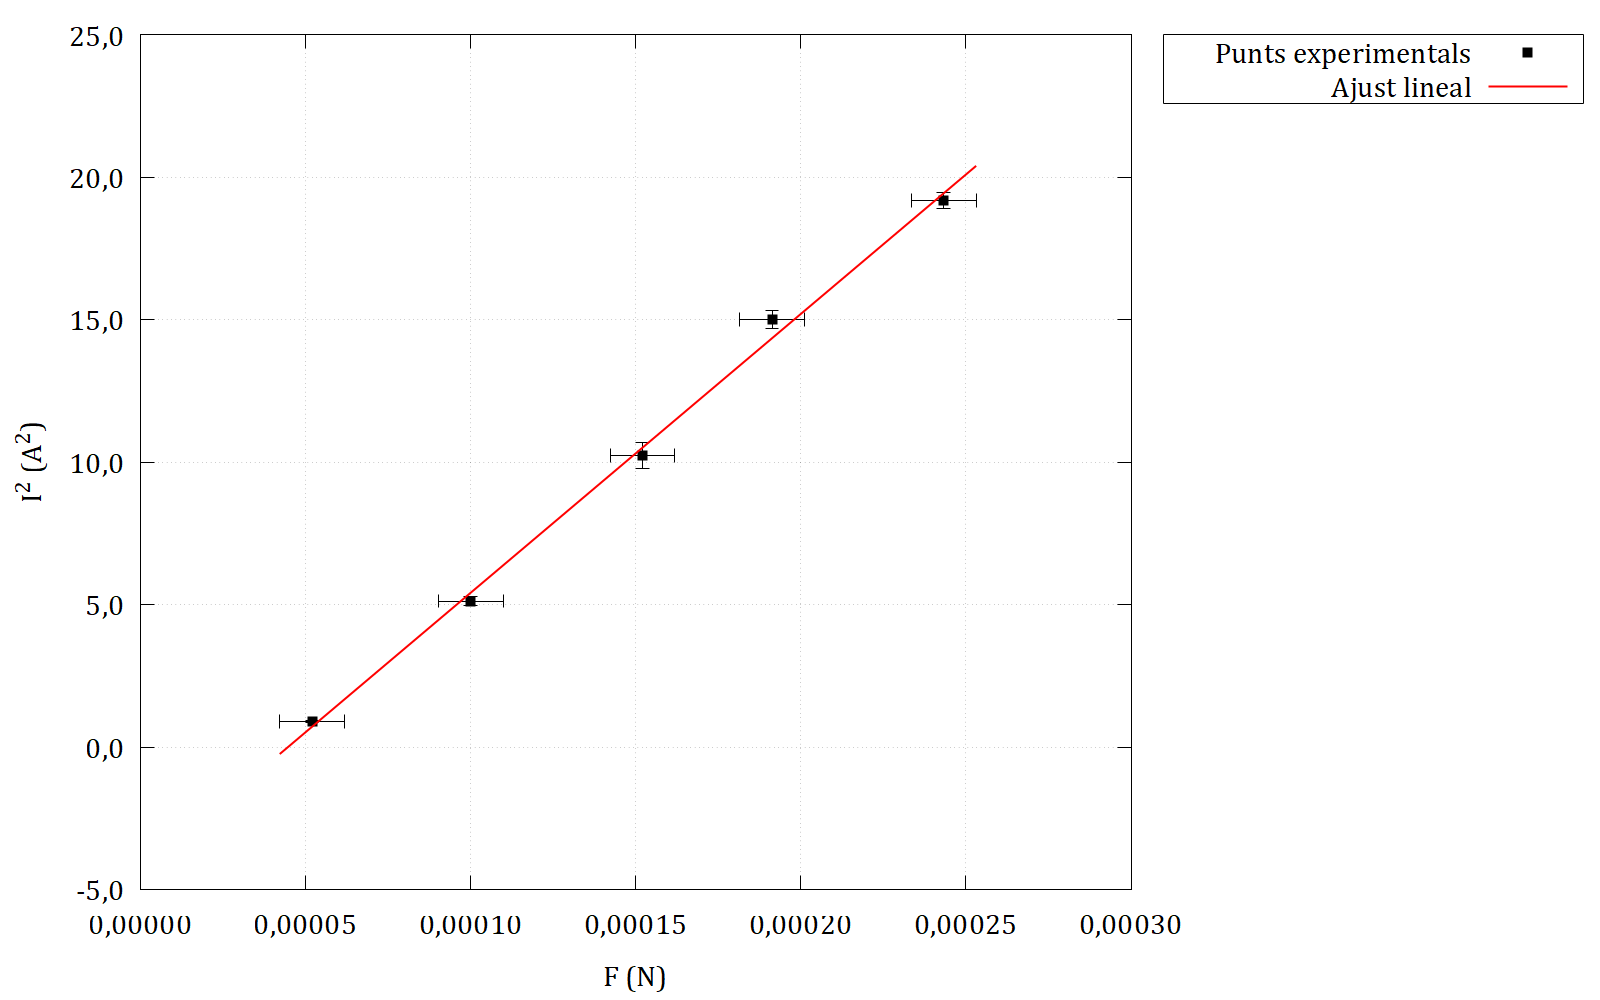
\includegraphics[width=0.8\linewidth]{screenshot020}
\caption{Força entre els dos fils en funció de la intensitat del corrent al quadrat. Dades de l'ajust lineal: $y=mx+n$, amb $m = (979 \pm 32)\cdot 10^{2}$ A$^2$$\cdot$N$^{-1}$ i $n = (-4,38\pm0,52)\cdot$ N$^{-1}$. Coeficient de correlació $R^2=0,997$. Notem que, en alguns punts, les barres d'error corresponents a l'eix de les $y$ són tan petites que no s'arriben a distingir.}
\label{fig:2.3}
\end{figure}

Si comparem aquest resultat amb el valor teòric de la permeabilitat magnètica
\begin{equation*}
	\mu_0^{teoric} = 4\pi\cdot 10^{-7} \text{ N/A$^2$} \approx 1,257\cdot10^{-6} \text{ N/A$^2$},
\end{equation*}
trobem que tenim un error relatiu del 36,64 \%.

\begin{figure}[H]
	\centering
	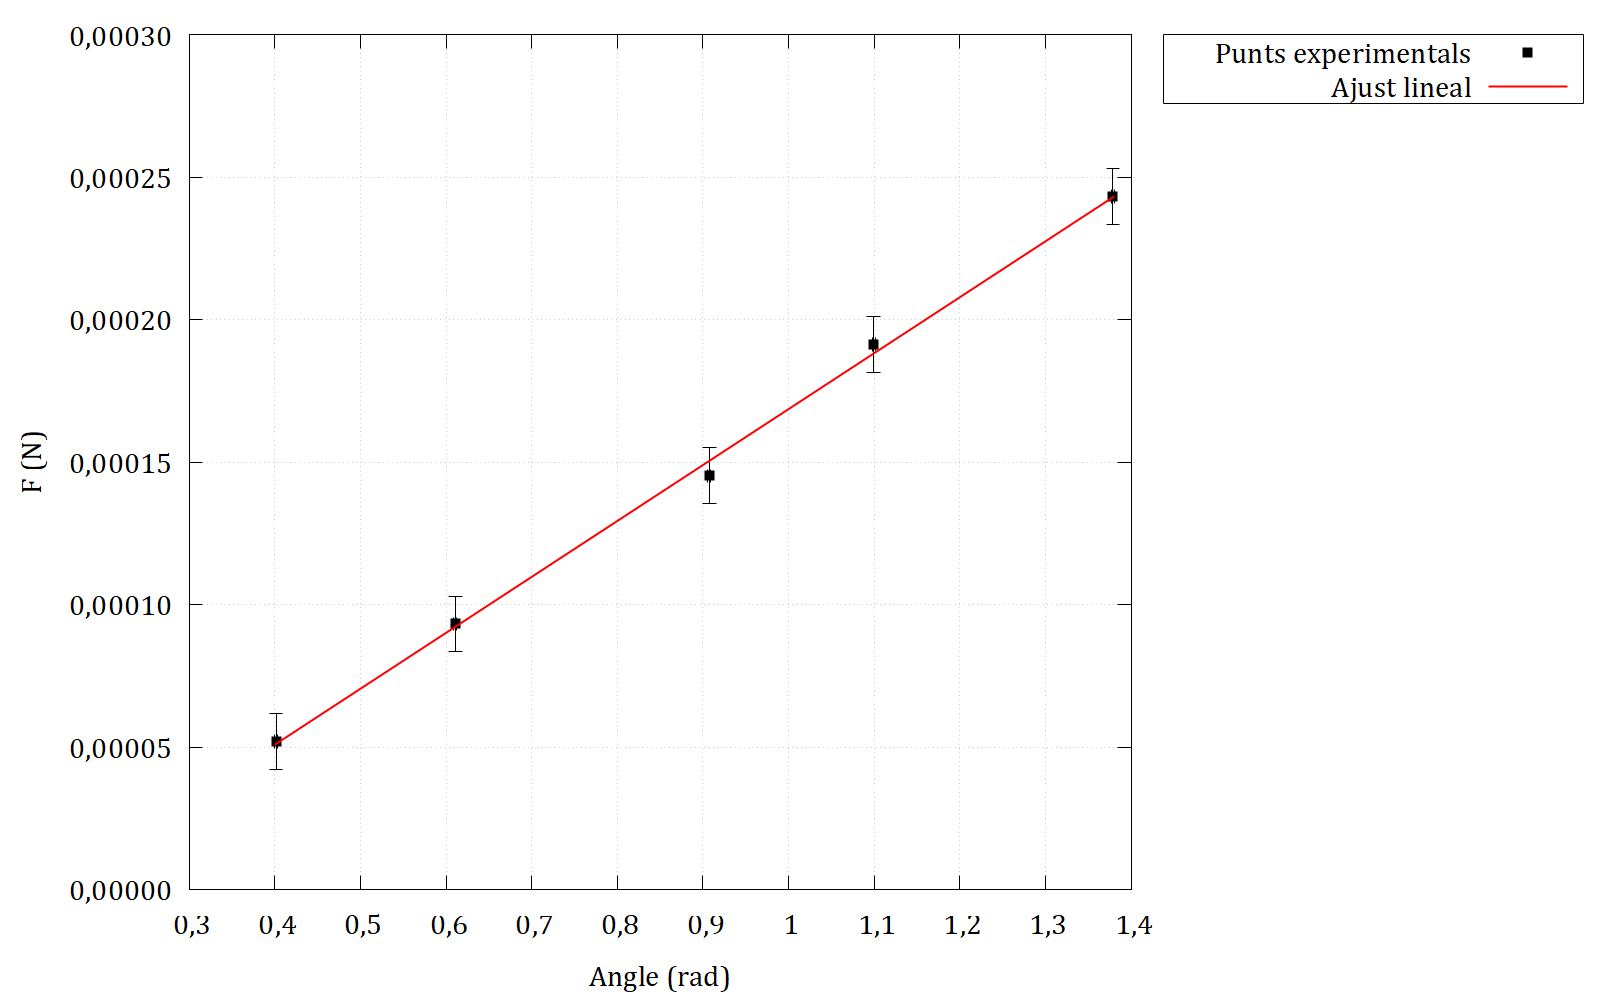
\includegraphics[width=0.8\linewidth]{screenshot017}
	\caption{Força en funció de l'angle de torsió $\theta$. Dades de l'ajust lineal: $y=mx+n$, amb $m=(1,9633\pm0,0047)\cdot10^{-4}$ N$\cdot$rad$^{-1}$ i $n=(-2,77\pm0,44)\cdot10^{-5}$ N. Coeficient de correlació $R^2=0,998$. Notem que, en alguns punts, les barres d'error corresponents a l'eix de les $x$ són tan petites que no s'arriben a distingir.}
	\label{fig:2.4}
\end{figure}

Per altra banda podem comparar amb el càlcul de $\mu_0$ mitjançant l'experiment del fil de torsió, és a dir, representant \textit{força vs. separació}. En aquest cas cal que determinem prèviament la constant de torsió del fil $k$, suposant que se satisfà que la força recuperadora és proporcional a l'angle de torsió $\theta$. A partir d'un seguit de mesures experimentals de $F$ i $\theta$ (veure annex \ref{an:c1}) podem fer un ajust lineal, tal i com es pot veure a la figura \ref{fig:2.4}, d'on es dedueix que
\begin{equation*}
	k = (1,9633\pm 0,0047)\cdot 10^{-4} \text{ N$\cdot$rad$^{-1}$}.
\end{equation*}
Ara, amb del valor d'aquesta constant, podem correlacionar les voltes necessàries del dial per equilibrar la balança en cada una de les configuracions a diferents distàncies, amb la força magnètica que produeix el corrent fixat de $I = (5,55 \pm 0,01)$ A que apliquem. 

De les mesures experimentals de $F$ vs. $1/r$ (essent $r$ la separació entre els fils) de l'annex \ref{an:c1}, podem fer un ajust lineal, tot trobant la recta de la figura \ref{fig:2.5}. Com que el pendent d'aquesta recta està directament relacionat amb $\mu_0$ (veure equació \eqref{eq:2.13}), en podem determinar el seu valor, tot trobant que 
\begin{equation*}
	\mu_0 = (2,206 \pm 0,036)\cdot 10^{-6}\text{ N$/$A$^2$}
\end{equation*}

\begin{figure}[H]
	\centering
	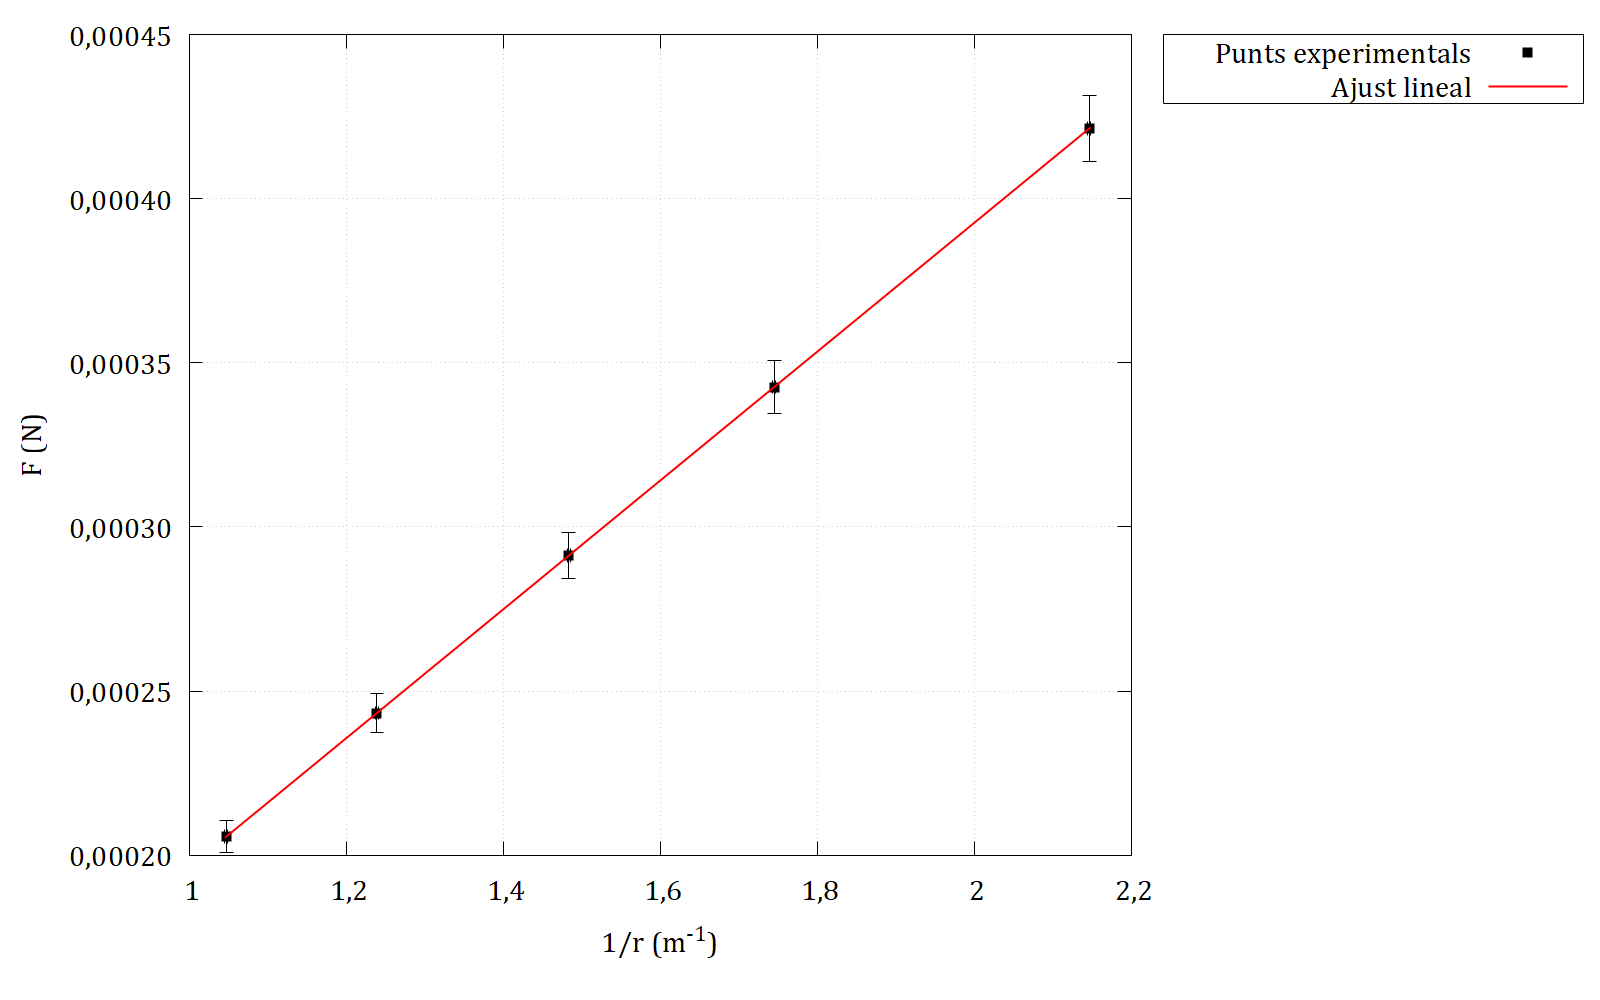
\includegraphics[width=0.9\linewidth]{screenshot018}
	\caption{Força en funció de $1/r$. Dades de l'ajust lineal: $y=mx+n$, amb $m = (3,298\pm0,051)\cdot 10^{-6} \text{ N$\cdot$m}$ i $n=(-1,194\pm 0,066)\cdot10^{-4} \text{ N}$. Coeficient de correlació $R^2=0,9993$. Notem que, en alguns punts, les barres d'error corresponents a l'eix de les $x$ són tan petites que no s'arriben a distingir.}
	\label{fig:2.5}
\end{figure}

Si comparem aquest resultat amb el valor de $\mu_0$ teòric trobem que cometem un error del 75,53 \%.

A la taula \ref{tab:2.1} podeu trobar agrupats els resultats dels dos experiments.
\begin{table}[h]
	\centering
	\caption{Resultats del càlcul de la permeabilitat magnètica del buit amb el corresponent error relatiu i el coeficient de correlació de l'ajust lineal per l'experiment de \textit{força vs. corrent} (1) i \textit{força vs. separació} (2).}
	\begin{tabular}{cccc}
		\toprule
		& $\mu_0$ (N/A$^2$) & Error Relatiu (\%) & $R^2$ \\
		\midrule
		\textbf{Valor Teòric} & $1,257\cdot10^{-6}$ & - & - \\
		\textbf{Experiment 1} & $(1,704\pm0,057)\cdot 10^{-6}$ & 36,64 & 0,997 \\
		\textbf{Experiment 2} & $(2,206\pm0,036)\cdot 10^{-6}$ & 75,53 & 0,9993 \\
		\bottomrule
	\end{tabular}
	\label{tab:2.1}
\end{table}

Podem veure que, clarament, dels dos experiments duts a terme, el primer (corresponent a l'estudi de la dependència de la força entre els fils en funció del corrent) és el que dóna un resultat de $\mu_0$ més proper al real. Que el segon experiment (corresponent a l'estudi de la dependència de la força entre els fils en funció de la separació entre aquests) presenti una desviació de més del doble que el darrer es pot justificar pel fet que, per fer aquest càlcul, hem hagut de determinar prèviament la constant de torsió del fil amb mesures efectuades amb la balança i, posteriorment, hem utilitzat aquestes dades per fer un ajust lineal i estudiar la dependència entre la força entre els fils en funció de la separació. Tot plegat fa que que l'error que tinguem en mesurar s'acumuli i es propagui a l'error comés en $\mu_0$. A més a més, no només l'error intrínsec del mètode es propaga, sinó que el possible error que tinguem per determinar $k$ també s'acumula a l'hora de fer l'ajust lineal dels punts de $F$ vs. $1/r$.

En general, considerem que és raonable que el segon experiment presenti un error major que el primer, que es fonamenta en mesures més directes (no cal efectuar dos ajusts lineals). El fet que, tot i això, l'error associat al primer sigui considerable, pot ser degut a la pròpia naturalesa de l'experiment. Recordem  que, al principi, per tal d'obtenir l'expressió que segueix el camp magnètic creat per un fil per on circula un corrent $I$, hem suposat que aquest fil era infinit, de manera que el camp generat és proporcional a $1/r$ en tots els punts (és a dir, té simetria perfectament cilíndrica) i, en particular, sobre l'altre fil i segons aquestes suposicions, el camp $\vec{B}$ és el mateix en tots els punts del darrer, ja que són paral·lels. Evidentment això últim no és cert per múltiples motius, entre els quals destaquem que: no tenim un fil infinit, ni tan sols la longitud ($L'$) del fil que crea el camp compleix que $L'\gg L$ (essent $L$ la longitud de l'altre fil), i existeixen efectes de vora (degut a que els fins no són infinits) que no hem considerat. Tot plegat fa que el $\vec{B}$ real no estigui generat ni estigui distribuït tal i com estem suposant, cosa que explicaria que ens sortís un valor de $\mu_0$ experimental més gran que el teòric, fem l'experiment que fem, ja que és un error directament relacionat amb el model considerat.

Tot i que tinguem un error associat a la mesura de $\mu_0$, sí que podem assegurar que la força entre els fils té un comportament que s'adequa al predit per l'equació \ref{eq:2.9} (és lineal), tal i com estableix el coeficient de correlació $R^2$, molt proper a 1 en els dos experiments. Sí que hem de remarcar, però, que tot i que l'equació \ref{eq2:10} no prediu l'existència de cap terme independent (ordenada d'origen) de manera que, per un valor $\theta = 0$ la força hauria de ser nul·la, els nostres resultats no indiquen totalment això, ja que a l'ajust lineal de la figura \ref{fig:2.4} es pot veure clarament que per $\theta = 0$, existeix una certa força 'residual'. Atribuïm aquest error a problemes relacionats amb el calibratge i l'ús de la balança; destaquem, però, que aquest error no hauria de ser d'especial rellevància en els nostres càlculs, ja que estem interessats només en el pendent de la recta (que no es veu influenciat per un canvi en l'ordenada d'origen), ja que és aquest el que ens permet arribar a un valor experimental de $\mu_0$. Una cosa molt similar es pot dir del terme independent que apareix en l'ajust $I^2$ vs. $F$.

 \textcolor{red}{\textbf{SEGUIR COMENTANT COSES I TAL. ideas per dir:}
 	\begin{itemize}
 		\item Les dues R's són "bones" (revisar conveni per quants decimals posar). He mirado en bastantes sitios y pone que entre 2 y 3 segun el caso (nunca he visto 4 deciameles), pero no estoy del todo seguro
 		\item Com a mínim els resultats són de l'ordre del valor real! creo  que lo pondria en conclusiones esto
 	\end{itemize}}



\subsection{Camp magnètic terrestre}
Contràriament als apartats anteriors, en aquest cas situem els conductors perpendiculars a la direcció nord-sud de la Terra. Això ens permet mesurar únicament la component horitzontal del camp magnètic terrestre ja que, com es pot observar a la figura \ref{fig2:6}, la força causada per aquesta component és la que podem mesurar equilibrant la balança amb el dial. Notem com, per contra, la força corresponent a la component vertical del camp magnètic terrestre no pot ser mesurada amb aquest mateix procediment.

\begin{figure}[H]
	\centering
	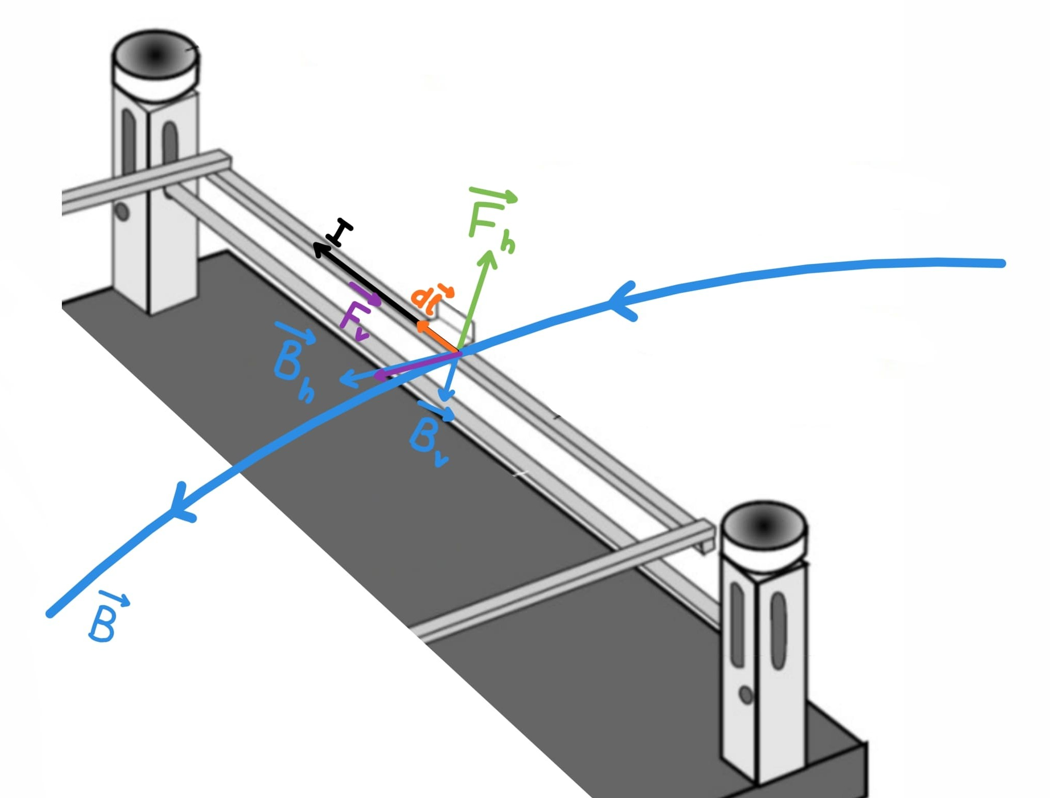
\includegraphics[width=0.35\linewidth]{screenshot019}
	\caption{Diagrama de forces que crea el camp magnètic terrestre a la balança. La força verda $F_h$ és la corresponent a la component horitzontal de $\vec{B}$.}
	\label{fig2:6}
\end{figure}


A partir de les mesures experimentals recollides a l'annex \ref{an:c1} de l'angle necessari per equilibrar la balança per a diferents valors d'intensitat, trobem que la component horitzontal del camp magnètic de la Terra és
\begin{equation*}
	B=(3,11 \pm 0,22)\times 10^{-5} \text{ T}.
\end{equation*}
El valor teòric és de 25053 nT, proporcionat per la pàgina web \textit{World Magnetic Model 2025 Calculator}\cite{ref2} calculat per una latitud i una longitud de (41,50057812688948, 2,1094089949997366), respectivament, i una alçada de 185 m sobre el nivell del mar. 

L'error relatiu, doncs, del valor experimental respecte el teòric és d'un 24,2 \%. Aquest percentatge el considerem acceptable per les limitacions que presenten les mesures que comentarem a continuació. A tot això, notem que el resultat experimental és del mateix ordre de magnitud que el teòric.

Les principals fonts d'error de la nostra mesura del camp magnètic rauen en la instrumentació utilitzada. La balança emprada no és d'elevada precisió, de manera que les mesures estan molt exposades a mínimes pertorbacions, ja siguin corrents d'aire i/o vibracions de la taula de treball. També cal considerar la possibilitat que la posició dels conductors no sigui exactament perpendicular a la direcció nord-sud.

Una altra limitació important relacionada amb l'instrument és la seva calibració. Tal com es va observant a mesura que es realitza la pràctica, a quasi cada apartat de la pràctica cal tornar a calibrar la balança. Això ens indica que, durant la manipulació de l'aparell, aquesta es descalibra lleugerament.

Finalment, és clar que el nombre de mesures preses és limitat. L'error relatiu, doncs, podria reduir-se mesurant el camp per més valors d'intensitat, de manera que la mitjana aritmètica donaria, en principi, un resultat més fiable.


\section{Conclusions}
En aquesta pràctica hem pogut analitzar, a partir de dos experiments diferents, l'equació que governa la força que es fan dos fils (de longitud $L$, suposada suficientment gran com per assumir que són infinits) pels quals hi circula un corrent elèctric, deduïda a partir de la llei de Biot i Savart. Els resultats extrets ens han permès estimar el valor de la permeabilitat magnètica del buit $\mu_0$, seguint dues metodologies diferents. En un cas hem mantingut la separació entre els fils constant i hem mesurat la dependència de la força (mesurada equilibrant la balança de la figura \ref{fig:2.1} amb peces metàl·liques de diferents masses) amb el quadrat de la intensitat; en un segon cas hem deixat el corrent fixat i hem estudiat com variava la força (mesurada equilibrant la balança de la figura \ref{fig:2.1} usant el dial i la constant de torsió del fil d'acer, trobada prèviament) en alterar la separació $r$ entre fils. A partir de vàries mesures (de $F$, $I$ i $r$ en funció del cas), hem pogut fer un ajust lineal que ens ha permès trobar un valor de $\mu_0$, directament relacionat amb el pendent de les rectes de regressió, en cada situació.

Dels dos experiments anteriors, hem vist que, en els dos casos, s'obtenen valors que són de l'ordre de la permeabilitat magnètica del buit teòrica, essent l'error de la segona experiència molt més gran ($\approx$ 76 \%) que l'error del primer cas ($\approx$ 37 \%). Atribuïm aquests errors, com hem discutit prèviament, a les múltiples limitacions del model emprat i de l'experiment dut a terme, entre les quals destaquem que: el model considerat no reflexa completament la naturalesa del sistema (ja que els dos fils no són estrictament infinits i cal considerar efectes de vora, que alteren la forma que pren el camp $\vec{B}$ i, en conseqüència, la força entre els dos fils), i que el muntatge de la balança era summament sensible a que es produïssin problemes relacionats amb el calibratge. En particular, pel segon experiment hem hagut de trobar prèviament un seguit de valors de la força $F$ vs. l'angle de torsió del fil $\theta$ per tal de trobar la constant de torsió $k$ (usant la llei de Hook, $F=k\theta$), a partir de la qual després hem pogut ajustar linealment les dades de $F$ vs. $1/r$. La necessitat de fer tantes mesures (i dos ajusts lineals) és una font d'error afegida que només afecta al segon experiment i que explicaria que tinguem un error en $\mu_0$ tan gran (respecte l'altre cas).  

Més enllà de tot això, també hem mesurat, a partir del mateix muntatge però canviant l'orientació dels fils conductors, la component horitzontal del camp magnètic terrestre al laboratori, a partir de mesures de l'angle de torsió del fil $\theta$ i de la intensitat que passava per un dels fils usant l'equació \eqref{eq:2.9}. Fent el promig de totes les mesures hem pogut estimar la component horitzontal del camp magnètic terrestre, amb un error del 24,2 \% respecte del valor teòric, proporcionat per la pàgina web \textit{World Magnetic Model 2025 Calculator} \cite{ref2}. L'error associat, novament, està relacionat amb les limitacions del muntatge i del model teòric esmentades però, tot i això, hem sigut capaços d'aconseguir resultats de l'ordre dels predits teòricament.

\chapter{Circuit RLC en sèrie}

\begin{chapterabstract}
	En aquesta pràctica estudiem el comportament del circuit més elemental que presenta oscil·lacions: el circuit RLC (resistència + condensador + bobina) en serie. El nostre objectiu principal és visualitzar, mitjançant un oscil·loscopi, les diferents solucions de l'equació diferencial de segon ordre associada a aquest sistema de gran interès físic.
\end{chapterabstract}

\section{Introducció i fonament teòric}

\subsection{Explicació qualitativa}

\begin{figure}[h]
	\centering
	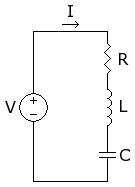
\includegraphics[width=0.15\linewidth]{screenshot014}
	\caption{Esquema d'un circuit RLC.}
	\label{fig:3.1}
\end{figure}

Per entendre per què aquest tipus de circuits (veure figura \ref{fig:3.1}) presenten oscil·lacions considerem, inicialment, que no tenim cap resistència i que el condensador es troba totalment carregat\footnote{Podeu trobar una animació d'aquest circuit a \url{https://commons.wikimedia.org/wiki/File:Tuned_circuit_animation_3.gif}.}. En connectar les plaques del condensador a la bobina, comença a circular una intensitat $I$ per aquesta. La variació de $I$ provoca, en virtut de la llei de Lenz
\begin{equation}
	\varepsilon = - \dv{}{t}\int_S \vec{B} \cdot \mathrm{d}\vec{s} \label{eq:3.1},
\end{equation}
una força electromotriu induïda als extrems de la bobina que s'oposa a l'augment de corrent. Com que la resistència $R$ és nul·la el potencial a la bobina serà igual i de signe contrari al potencial entre les plaques del condensador (si no fos així tindríem una intensitat infinita circulant per la bobina). 

Tanmateix, mentre el condensador es descarrega, la intensitat va augmentant, de forma que, quan el condensador està totalment descarregat (i, per tant, el potencial és zero entre les dues plaques), la intensitat és màxima. Com que és impossible que el corrent s'anul·li de sobte (ja que implicaria una $\varepsilon$ infinita), continua circulant intensitat en el mateix sentit i el condensador es carrega amb polaritat contrària a la de l'inici. 

Ara, el procés de càrrega del condensador fa que la intensitat disminueixi progressivament (el voltatge total del circuit ha de ser nul en tot moment); quan la intensitat arriba a zero la càrrega del condensador ha de ser necessàriament la mateixa que a l'inici, ja que, com que la resistència òhmica del circuit és nul·la, no hem tingut pèrdues energètiques associades a l'efecte Joule, però el potencial és de signe oposat. En tot aquest procés ha passat un \textit{semiperíode}. Seguidament torna a començar el procés de càrrega del condensador fins a tornar a arribar a la situació inicial; tot plegat explica per què el voltatge entre les plaques del condensador oscil·la indefinidament.

La capacitat $C$ del condensador és
\begin{equation}
	C = \frac{q}{V_C}, \label{eq:3.2}
\end{equation}
i l'autoinductància de la bobina és
\begin{equation}
	L = V_L \frac{\Delta t}{\Delta I}, \label{eq:3.3}
\end{equation}
on $q$ és la càrrega emmagatzemada al condensador, el quocient $\frac{\Delta t}{\Delta I}$ és la variació de temps per una certa variació de la intensitat i  $V_L$ i $V_C$ són els voltatges associats a la bobina i al condensador, respectivament. Aquestes dues magnituds, que depenen únicament de la geometria del sistema considerat, són de vital importància per descriure com seran aquestes oscil·lacions. Notem que: 
\begin{itemize}
	\item Com més petita sigui la capacitat $C$ del condensador, més ràpidament es descarregarà (té menys càrrega).
	\item Com més petita sigui l'autoinductància $L$ de la bobina, més variació en la intensitat és necessària per donar una mateixa força electromotriu $\varepsilon$, de manera que també més ràpidament es descarregarà el condensador.
\end{itemize}
Si tenim presents aquests dos efectes, fàcilment podem arribar a la conclusió que com menors siguin l'autoinductància i la capacitat del circuit, més alta serà la freqüència d'oscil·lació.

Totes aquestes consideracions són assumint que la resistència del circuit és negligible. En cas que no ho sigui (com en el cas que estudiem) el voltatge a la bobina i al condensador seran lleugerament diferents i, per cada oscil·lació, perdrem part de l'energia del sistema en forma de calor (per l'efecte Joule). Si la resistència es fa molt gran, deixaran d'haver-hi oscil·lacions.

\subsection{Equació general del circuit RLC}
Per circuits en sèrie els voltatges se sumen i les intensitats són iguals per a tots els elements del circuit, de forma que el voltatge total es correspondrà amb
\begin{equation}
	V = V_R + V_L + V_C = RI + L \dv{I}{t} + \frac{1}{C} \int I\mathrm{d}t, \label{eq:3.4}
\end{equation}
on hem emprat les expressions 
\begin{align}
	V_R & = RI, \\
	V_L & = L \dv{I}{t}, \\
	V_C & = \frac{1}{C} \int I \mathrm{d}t,
\end{align}
i on $I$ és la intensitat que circula pel circuit i $V_R$, $V_C$ i $V_L$ són els voltatges a la resistència, el condensador i la bobina, respectivament. 

Si derivem respecte del temps l'expressió \eqref{eq:3.4} i reorganitzem obtenim:
\begin{equation}
	\dv[2]{I}{t} + \frac{R}{L} \dv{I}{t}+\frac{1}{LC} = \frac{1}{L}\dv{V}{t}.\label{eq:3.8}
\end{equation}
Podem trobar dues expressions alternatives a aquesta darrera equació. Si ens interessa tenir una equació en funció del potencial als extrems de la resistència només cal que multipliquem per $R$; si ens interessa expressar-ho tot en funció del potencial al condensador hem de tenir en compte que
\begin{equation}
	I = C \dv{V_C}{t},
\end{equation}
de manera que obtenim les següents dues expressions alternatives:
\begin{align}
	\dv[2]{V_R}{t} + \frac{R}{L}\dv{V_R}{t} + \frac{1}{LC}V_R = \frac{R}{L} \dv{V}{t}, \\
	\dv[2]{V_C}{t} + \frac{R}{L}\dv{V_C}{t} + \frac{1}{LC}V_C=\frac{1}{LC}V. \label{eq:3.11}
\end{align}

\subsection{Règim permanent}
En aquest règim assumim que subministrem un senyal sinusoidal al circuit, de manera que:
\begin{equation}
	V(t) = V_{max} \sin (\omega t). \label{eq:3.12}
\end{equation} 
La solució de l'equació \eqref{eq:3.8} és també una ona sinusoidal:
\begin{equation}
	I(t) = I_{max}\sin(\omega t + \phi).
\end{equation}
Si expressem això en notació complexa\footnote{Denotem la unitat imaginària amb $j$ per evitar confusions amb la intensitat.}
\begin{align}
	I(t) & = I_{max} \mathrm{e}^{j(\omega t + \phi)}, \\
	V(t) & = V_{max} \mathrm{e}^{j\omega t},
\end{align}
i ho substituïm a l'equació \eqref{eq:3.4} tenim
\begin{equation}
	V(t) = \left[R+j \left(L\omega - \frac{1}{C\omega}\right)\right]I(t),
\end{equation}
que ens permet, per tal de tenir una expressió anàloga a la llei d'Ohm de la forma $V=ZI$, definir la impedància $Z$ (mesurada en $\Omega$):
\begin{equation}
	Z \equiv R+j\left(L\omega - \frac{1}{C\omega}\right).
\end{equation}
Notem que, com que, si prenem mòduls
\begin{equation}
	\abs{I} = \frac{\abs{V}}{\abs{Z}} = \frac{\abs{V}}{\sqrt{R^2+\left( L\omega - \frac{1}{C\omega}\right)^2 }},
\end{equation}
veiem que la intensitat serà màxima quan se satisfaci que $L\omega - \frac{1}{C\omega} = 0$. La freqüència \textit{pròpia} o \textit{de ressonància} del circuit RLC és aquella tal que aquesta darrera condició se satisfà i es defineix segons\footnote{Fem notar que $\abs{Z(\omega_0)} = R$.}:
\begin{equation}
	\omega_0^2 \equiv \frac{1}{LC} \label{eq:3.19}.
\end{equation}

\subsection{Règim transitori}
En aquest règim assumim que se subministra al circuit RLC un senyal de tipus rectangular de període $T'$:
\begin{equation}
	V(t) = 
	\begin{cases}
		E & \text{si } 0 < t < T'/2 \\
		0 & \text{si } T'/2 < t < T' \label{eq:3.20}
	\end{cases}
\end{equation}
Ens interessa solucionar, amb aquesta funció $V(t)$, l'equació \eqref{eq:3.11}. És una EDO de primer ordre i no homogènia; la solució serà la suma de la solució general per l'EDO homogènia més una solució particular:
\begin{itemize}
	\item És immediat veure que una solució particular és $V_C = V(t)$.
	\item Per trobar la solució de l'equació homogènia cal solucionar
	\begin{equation}
		x^2 + \frac{R}{L}x + \frac{1}{LC} = 0, \label{eq:3.21}
	\end{equation}
	que tindrà diferents solucions en funció de com sigui el discriminant
	\begin{equation}
		\Delta = \left(\frac{R}{L}\right)^2-\frac{4}{LC}.
	\end{equation}
\end{itemize}
Tenim els següents tres casos:
\begin{enumerate}
	\item Si $\Delta < 0$ ($R$'s petites), l'equació \eqref{eq:3.21} té com a solució
	\begin{equation}
		x = - \lambda \pm j\omega,
	\end{equation}
	essent $\lambda$ la \textit{constant d'esmorteïment}, definida segons
	\begin{equation}
		\lambda \equiv \frac{R}{2L}.
	\end{equation}
	De forma similar, definim la \textit{freqüència de pseudo-pulsació} com\footnote{Fixem-nos que si el circuit està poc amortit ($R\rightarrow 0$), aleshores $\omega \approx \omega_0$.}
	\begin{equation}
		\omega \equiv \sqrt{\omega_0 - \frac{1}{4}\left(\frac{R}{L}\right)^2}. \label{eq:3.25}
	\end{equation}
	Així mateix, tenint en compte la solució particular podem escriure la solució general de l'EDO com
	\begin{equation}
		V_C(t) = A \mathrm{e}^{-\lambda t}\cos(\omega t - \psi) + V(t),
	\end{equation}
	si imposem les condicions inicials adequades (a $t=0$ la diferència de potencial en el condensador i la intensitat del circuit són 0), acabem trobant
	\begin{equation}
		\boxed{V_C(t) = E \left[1-\sqrt{1+\left(\frac{\lambda}{\omega}\right)^2}\mathrm{e}^{-\lambda t}\cos(\omega t - \psi)\right]}. 
	\end{equation}
	Si només ens fixem en els punts extremals, on $\cos(\omega t - \psi) = \pm 1$, aleshores
	\begin{equation}
		\ln\abs{V_C(t_i)-E} = \ln\abs{A}-\lambda t. \label{eq:3.28}
	\end{equation}
	Aquesta darrera equació és l'equació d'una recta de pendent $-\lambda$. Ens permetrà, a partir d'un conjunt de mesures de $\ln\abs{V_C(t_i)-E}$ i $t$ determinar la constant d'esmorteïment.
	\item Si $\Delta > 0$ ($R$'s grans), la solució de \eqref{eq:3.21} és
	\begin{equation}
		x_{1,2} = -\frac{R}{2L}\pm \frac{1}{2}\sqrt{\Delta},
	\end{equation}
	de manera que la solució general a l'EDO és
	\begin{equation}
		\boxed{V_C(t) = A_1 \mathrm{e}^{x_1t}+A_2\mathrm{e}^{x_2t}+V(t)},
	\end{equation}
	amb $A_1$ i $A_2$ dues constants a determinar (de nou, usant les condicions inicials).
	\item Si $\Delta = 0$ tenim que la resistència es correspon amb la \textit{resistència crítica}
	\begin{equation}
		R_{crit} = 2\omega_0L = 2\sqrt{\frac{L}{C}} \label{eq:3.31}.
	\end{equation}
	La solució general de l'EDO (un cop s'han imposat les condicions inicials) és
	\begin{equation}
		\boxed{V_C(t) = E[1-\mathrm{e}^{-\lambda t}(t+1)]}.
	\end{equation}
\end{enumerate}

\subsection{Desfasament entre voltatges}
El guany en voltatge a la resistència, és a dir, la relació entre el voltatge a la resistència i el voltatge d'entrada es defineix segons
\begin{equation}
	T_R = \frac{V_R}{V} = \frac{R}{R+j(L\omega - \frac{1}{C\omega})} \label{eq:3.33}.
\end{equation}
Si $\phi$ és el \textit{desfasament} entre el voltatge d'entrada i el corresponent a la resistència, aleshores tenim
\begin{equation}
	T_R = \abs{T_R}\mathrm{e}^{j \phi},
\end{equation}
on
\begin{equation}
	\tan \phi = -\frac{L\omega - \frac{1}{C\omega}}{R}.
\end{equation}
D'aquí es pot deduir que:
\begin{itemize}
	\item Si $\omega > \omega_0$ $\Rightarrow$ $-\frac{\pi}{2}<\phi<0$. $V_R$ està enrederit respecte del voltatge d'entrada.
 	\item Si $\omega < \omega_0$ $\Rightarrow$ $0<\phi<\frac{\pi}{2}$. $V_R$ està avançat respecte del voltatge d'entrada.
\end{itemize}
En particular, si $\omega = \omega_0$ les dues ones estan en fase (estem en situació de ressonància) i tenim que $\abs{T_R} = 1$ (el guany és màxim).

\subsection{Freqüències de tall i amplada de banda}
Les freqüències de tall es defineixen com aquelles freqüències $\omega_c$ tals que se satisfà que
\begin{equation}
	\abs{T_R(\omega_c)} = \frac{1}{\sqrt{2}}.
\end{equation}
Aquestes freqüències ens permeten estudiar l'amplada de banda del sistema. Si usem la definició del guany a la resistència donada a \eqref{eq:3.33} tenint present la definició de la freqüència de ressonància (equació \eqref{eq:3.19}) trobem
\begin{equation}
	\left(\frac{\omega_c}{\omega_0}\right)^2 \pm \frac{R}{L\omega_0}\left(\frac{\omega_c}{\omega_0}\right) -1=0,
\end{equation}
de manera que tenim dues freqüències de tall, $\omega_1$ i $\omega_2$, que satisfan 
\begin{align}
	\omega_2-\omega_1 & = \frac{R}{L}, \label{eq:3.38} \\
	\omega_2 \cdot \omega_1 & = \omega_0^2 \label{eq:3.39}.
\end{align}
Fixem-nos que l'amplada de banda es correspon amb la diferència entre les dues freqüències de tall, de forma que
\begin{equation}
	\Delta \omega = \frac{R}{L}.
\end{equation}

\section{Metodologia experimental}

\subsection{Estudi del règim permanent}\label{expermento permanente}

Comencem muntant el circuit de la figura \ref{fig:3.2}\footnote{Les figures corresponents als circuits i al muntatge experimental han estat extretes dels \textit{Guions de les pràctiques de l'assignatura de Laboratori d'Electromagnetisme}\cite{ref3}}. Usem una bobina de $L = 22$ mH, un condensador de $C = 15$ nF, una font de corrent altern que ens subministra una senyal del tipus \eqref{eq:3.12}  i, inicialment, una resistència de $R = 2700$ $\Omega$. Efectuem les mesures amb un oscil·loscopi de doble traça; a la figura, $Y_A$ i $Y_B$ representen els dos canals d'aquest.

\begin{figure}[h]
	\centering
	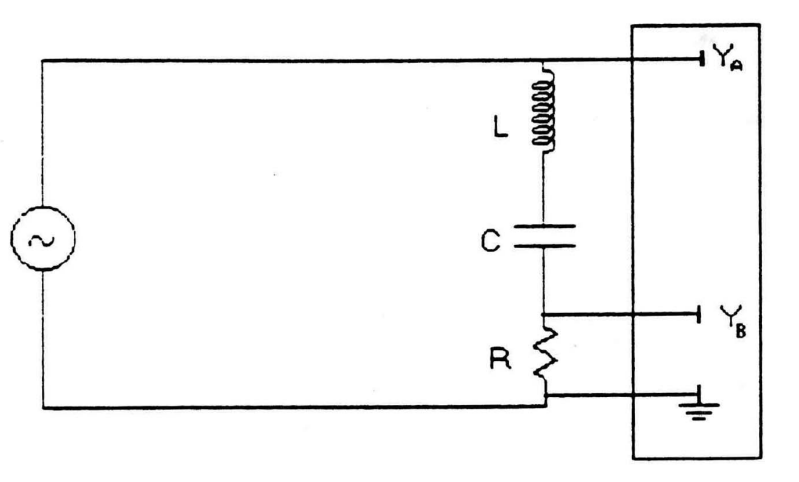
\includegraphics[width=0.5\linewidth]{screenshot005}
	\caption{Esquema del circuit usat pel règim permanent.}
	\label{fig:3.2}
\end{figure}

Variem la freqüència de la font fins que els dos senyals a l'oscil·loscopi estan en fase (usant el model DUAL del darrer). Aquesta freqüència es correspon amb la freqüència de ressonància. La comparem amb la freqüència de ressonància teòrica (en Hz)
\begin{equation}
	f_0 = \frac{1}{2\pi}\sqrt{\frac{1}{LC}}, \label{eq:3.41}
\end{equation}
i mesurem el guany $\abs{T_R(\omega_0)}$ corresponent a aquesta freqüència.

Mesurem les dues freqüències de tall $f_1$ i $f_2$ (en Hz)\footnote{Recordem que són les freqüències tals que $\abs{T_R(\omega_c)} = \frac{1}{\sqrt{2}}$.}. Comparem els valors mesurats amb els valors teòrics (a partir de la resolució del sistema d'equacions donat per \eqref{eq:3.38} i \eqref{eq:3.39}). Repetim tot el procediment canviant la resistència per una de $R = 270$ $\Omega$.

\subsection{Estudi del règim transitori}
Muntem el circuit de la figura \ref{fig:3.3}. Usem una bobina de $L = 33$ mH, un condensador de $C = 330$ pF, una font que ens subministri una senyal tipus \eqref{eq:3.20} i una resistència de $R = 180$ $\Omega$.

\begin{figure}[h]
	\centering
	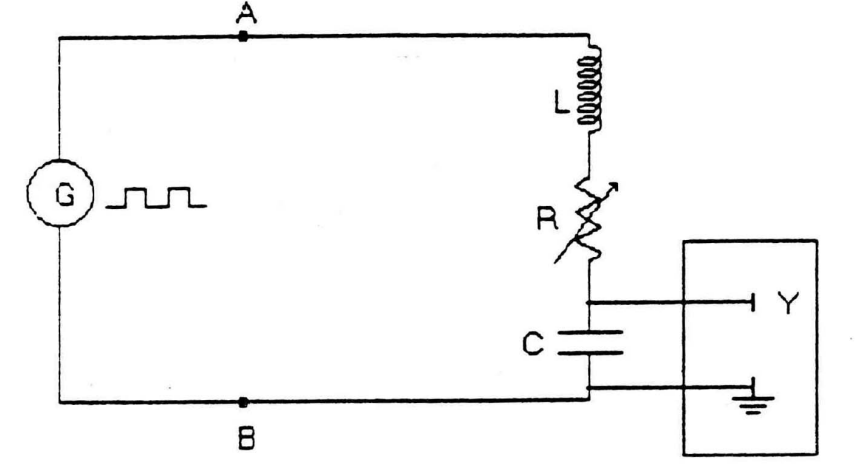
\includegraphics[width=0.5\linewidth]{screenshot006}
	\caption{Esquem del circuit usat pel règim transitori.}
	\label{fig:3.3}
\end{figure}

Fixem la freqüència del generador de forma que a cada període d'aquest, $T_{generador}$, apareguin 10 oscil·lacions de període $T$ ($f = \frac{T}{10}$), essent aquest període $T$ el corresponent a la freqüència de pseudo-pulsació, calculat usant l'equació \eqref{eq:3.25} i que
\begin{equation}
	T = \frac{2\pi}{\omega}.
\end{equation}
Seguidament mesurem el període $T$ amb l'oscil·loscopi. 

Canviem la resistència fixa per una de variable, que pot donar resistències de 0 a 100 k$\Omega$. Estudiem els casos $R<R_c$, $R=R_c$ i $R>R_c$ (on $R_c$ és la resistència crítica, donada per l'equació \eqref{eq:3.31}), de forma que podem veure les 3 solucions per a l'EDO del circuit RLC en règim transitori. Finalment, amb els valors recollits de $V_C$ i de $t$, calculem, via l'equació \eqref{eq:3.28}, el valor de la constant d'esmorteïment $\lambda$.


\section{Resultats i discussió}
\textcolor{red}{tengo que poner las incertidumbres bien a bastantes cosas, ahora no me apetece}\\
Per poder comparar i entendre si els nostres resultats son correctes lo primer de tot serà predir amb el que sabem d'electro el que creiem que passarà. Tenim un circuit com el de la figura \ref{fig:3.2} amb $R=2660$ o $274$ $\Omega$, $L=22$ mH, $C=15$ nF i una font amb un voltatge d'entrada tipus $V(t) = V_{max}\sin(\omega t)$, la freqüència de ressonància del sistema ve donada per $\omega_0 = (LC)^{-1}$ (equació \ref{eq:3.19}), i les freqüències de tall ens les dona el sistema d'equacions definit per les equacions \ref{eq:3.38} i \ref{eq:3.39}, que si el resolem queda que:

\begin{eqnarray*}
	\omega_{1,2} = \frac{1}{2L} \left( \sqrt{4L^2\omega_0^2+R^2} \mp R \right)  
\end{eqnarray*}
Així podem calcular certes propietats del circuit, i també d'altres com $\text{T}_\text{R}(\omega)$:

\begin{table}[h]
	\centering
	\renewcommand{\arraystretch}{1.2}
	\caption{Valors teòrics del sistema}
	\begin{tabular}{lccccc}
		\toprule
		& $f_0$ (\text{Hz}) & $f_1$ (\text{Hz}) & $f_2$ (\text{Hz}) & $\abs{T_R(\omega_0)}$ & $\abs{T_R(\omega_{1,2})}$ \\ 
		\midrule
		$\mathbf{R = 2660\Omega}$ & 8761 $\pm$ 35 & 3391 $\pm$ 98 & 22634 $\pm$ 680 & 1 & $1/\sqrt{2}$\\ 
		$\mathbf{R = 274\Omega}$ & 8761 $\pm$ 35 & 7826 $\pm$ 35 & 9808 $\pm$ 91 & 1 & $1/\sqrt{2}$ \\
		\bottomrule
	\end{tabular}
\end{table}

\textcolor{red}{poner resultados necesarios para el régimen transitorio tmb}\\
Els recull de mesures experimentals es troben a l'annex \textcolor{red}{poner anexo}.

\subsection{Règim permanent}

\textbf{\textcolor{red}{IMPORTANT: Quins valors dels calculats, $f_{0,1,2}$ i $\abs{T_R}$ romanen iguals i quins canvien? Per què? Si volguéssim un circuit amb una banda de pas estreta, quina resistència escollim?}} (pregunta del guió, a algun lloc s'ha de contestar)

Una vegada s'han mesurat les freqüències de ressonància i de tall, i els valors dels voltatges d'entrada i de la resistència just com s'explica a la secció \ref{expermento permanente} podem obtenir els següents valors experimentals directament de l'oscil·loscopi:

\begin{table}[h]
	\centering
	\renewcommand{\arraystretch}{1.2}
	\caption{Valors experimentals del sistema}
	\label{val exp trans}
	\begin{tabular}{lcccccc}
		\toprule
		& $f_0$ (\text{Hz}) & $f_1$ (\text{Hz}) & $f_2$ (\text{Hz}) & $\abs{T_R(\omega_0)}$ & $\abs{T_R(\omega_{1})}$ & $\abs{T_R(\omega_{2})}$ \\ 
		\midrule
		$\mathbf{R = 2660\Omega}$ & 8960 $\pm$ 1 & 2860 $\pm$ 1 & 23460 $\pm$ 1 & 1 $\pm$ 0,0075 & 0,72340 $\pm$ 0,0066 & 0,72340 $\pm$ 0,0066\\ 
		$\mathbf{R = 274\Omega}$ & 8860 $\pm$ 1 & 8040 $\pm$ 1 & 9830 $\pm$ 1 & \textcolor{magenta}{0,87647 $\pm$ 0,0078} & 0,70588 $\pm$ 0,0072 & \textcolor{magenta}{0,88235$\pm$ 0,0078}\\
		\bottomrule
	\end{tabular}
\end{table}


\begin{table}[h]
	\centering
	\renewcommand{\arraystretch}{1.2}
	\caption{Error en les mesures respecte els valors teòrics esperats}
	\label{error exp trans}
	\begin{adjustbox}{max width=\textwidth}
	\begin{tabular}{lcccccc}
		\toprule
		& $f_0$ (\text{Hz}) & $f_1$ (\text{Hz}) & $f_2$ (\text{Hz}) & $\abs{T_R(\omega_0)}$ & $\abs{T_R(\omega_{1})}$ & $\abs{T_R(\omega_{2})}$ \\ 
		\midrule
		$\mathbf{R = 2660\Omega}$ & (2,27 $\pm$ 0,41$)\%$ & (15,66 $\pm$ 2,43$)\%$ & (3,65 $\pm$ 3,11$)\%$ & (0,00 $\pm$ 0,75$)\%$ & (2,30 $\pm$ 0,93$)\%$ & (2,30 $\pm$ 0,93$)\%$\\ 
		$\mathbf{R = 274\Omega}$ & (1,13 $\pm$ 0,41$)\%$ & (2,73 $\pm$ 0,47$)\%$ & (0,22 $\pm$ 0,93$)\%$ & \textcolor{magenta}{(12,35 $\pm$ 0,000089$)\%$} & (0,17 $\pm$ 1,02$)\%$ & \textcolor{magenta}{(24,78 $\pm$ 1,11$)\%$}\\
		\bottomrule
	\end{tabular}
	\end{adjustbox}
\end{table}

A la taula \ref{val exp trans} es troben els resultats de l'experiment, com els valors son bastant variats farem l'anàlisi d'aquestes dades sobretot a partir del percentatge d'error respecte als valors teòricament predits que adjuntem a la taula \ref{error exp trans}. \\

Amb el procediment experimental seguit hem aconseguit recrear bastant bé tant la freqüència pròpia del sistema com les freqüències de tall amb els dos valors de la resistència. Encara que en general els resultats estan aproximadament dins del que esperàvem notem que tenim dos grans errors, un en $f_1$ per a $R = 2660\Omega$ que tenim un error considerablement gran, del $(15,66 \pm 2,43) \%$, i l'altre pels valors de $\abs{T_R(\omega_0)}$ i $\abs{T_R(\omega_2)}$, que temim uns errors del $(12,35 \pm 0,000089) \%$ i $(24,78 \pm 1,11) \%$ respectivament. Comentem un a un:\\

 L'error $f_1$ per $R = 2660\Omega$ es degut a que al laboratori no vam anar amb molta cura en seleccionar les freqüències, l'oscil·loscopi pot donar freqüències amb molta precisió però nosaltres donat que les freqüències son de l'ordre dels milers vam considerar que anar fent salts de 50Hz en 50Hz o 100Hz en 100Hz era bona idea, a la practica podia semblar que això ja era suficient però acabem de veure que no. Ho vam considerar així ja que experimentalment tampoc s'aprecia un gran salt en $\abs{T_R(\omega)}$ al moure la freqüència de 100 en 100Hz (ho podem veure a la figura \textcolor{red}{poner ref}), el problema es que $\abs{T_R(\omega)}$ a freqüències molt baixes o molt altes comparades amb $f_0$, com ho son $f_1$ i $f_2$, $\abs{T_R(\omega)}$ canvia lentament (això es dedueix de la forma de l'equació \ref{eq:3.33}), i a més $\abs{T_R(\omega)}$ està acotat en $(0,1]$, per lo que el canvi en $\abs{T_R(\omega)}$ a aquests oredes de frecuencia no s'aprecia molt. Aixó explica que en algunes freqüències tinguem un error relativament alt però per aquestes mateixes freqüències l'error en $\abs{T_R(\omega)}$ no sigui molt important. \\

El que es important observar es que hem aconseguit reproduir perfectament els ordes de magnitud de totes les freqüències i veure com la ganància en el voltatge de la resistència va canviant amb aquestes, sent la màxima possible en la freqüència de ressonància del sistema.    

\textcolor{red}{quitar lila}\\
\textcolor{red}{algo raro hay con $\abs{T_R(\omega_0)}$ y $\abs{T_R(\omega_{2})}$ para $\mathbf{R = 274\Omega}$, son muy diferentes de lo que debería, errores del 12 y 25$\%$....., pero es que si lo recalculo con otro método esas dos dan muy guai, pero entonces es $\abs{T_R(\omega_1)}$ que para $\mathbf{R = 2660\Omega}$ y $\mathbf{R = 274\Omega}$ da mal con errores del 11 y 13$\%$, QUE PASA!! pq siempre hay dos que dan mal......., :(}\\
\textcolor{red}{A ver, vamos a probar a recalcular todo esto pero con otro método. Los valores de las frecuencias no hay nada que hacerle porque son las que nos soltaba directamente el osciloscopio al hacer el experimento e ir variando $f$ poco a poco para que las ondas estén en fase para medir $f_0$, y ir variando $f$ para que los voltajes pico cumplan la relación de $1/\sqrt{2}$ para medir $f_{1,2}$. Pero que en las ganancias $\abs{T_R(\omega)}$ haya errores del 24$\%$ no se como justificarlo.}\\

\textcolor{red}{Para “arreglar eso”, vamos a calcular las $\abs{T_R(\omega)}$ de otra manera, en vez de hacer la división de $V_R/V_E$, donde estos dos voltajes de nuevo son valores que te suelta directamente el osciloscopio al hacer el experimento lo que haré es aprovechar que tenemos medidas experimentalmente $f_{0,1,2}$ y utilizo la formula \ref{eq:3.33} para calcular las $\abs{T_R(\omega)}$, con este método los resultados son: (recordar que las $f_{0,1,2}$ son exactamente las mismas que antes)}\\

\begin{table}[H]
	\centering
	\renewcommand{\arraystretch}{1.2}
	\caption{Valors experimentals del sistema (2n mètode)}
	\begin{tabular}{lcccccc}
		\toprule
		& $f_0$ (\text{Hz}) & $f_1$ (\text{Hz}) & $f_2$ (\text{Hz}) & $\abs{T_R(\omega_0)}$ & $\abs{T_R(\omega_{1})}$ & $\abs{T_R(\omega_{2})}$ \\ 
		\midrule
		$\mathbf{R = 2660\Omega}$ & - & - & - & 0,999791 $\pm$ 0,000076 & \textcolor{magenta}{0,626 $\pm$ 0,015} & 0,690 $\pm$ 0,014\\ 
		$\mathbf{R = 274\Omega}$ & - & - & - & 0,9951 $\pm$ 0,0035 & \textcolor{magenta}{0,796 $\pm$ 0,014} & 0,700$\pm$ 0,012\\
		\bottomrule
	\end{tabular}
\end{table}


\begin{table}[H]
	\centering
	\renewcommand{\arraystretch}{1.2}
	\caption{Error en les mesures respecte els valors teórics esperats (2n mètode)}
	\begin{adjustbox}{max width=\textwidth}
		\begin{tabular}{lcccccc}
			\toprule
			& $f_0$ (\text{Hz}) & $f_1$ (\text{Hz}) & $f_2$ (\text{Hz}) & $\abs{T_R(\omega_0)}$ & $\abs{T_R(\omega_{1})}$ & $\abs{T_R(\omega_{2})}$ \\ 
			\midrule
			$\mathbf{R = 2660\Omega}$ & - & - & - & (0,0209 $\pm$ 0,0076$)\%$ & \textcolor{magenta}{(11,49 $\pm$ 2,06$)\%$} & (2,42 $\pm$ 1,94$)\%$\\ 
			$\mathbf{R = 274\Omega}$ & - & - & - & (0,49 $\pm$ 0,35$)\%$ & \textcolor{magenta}{(12,58 $\pm$ 2,01$)\%$} & (0,98 $\pm$ 1,72$)\%$\\
			\bottomrule
		\end{tabular}
	\end{adjustbox}
\end{table}


podem veure que els valors són pràcticament iguals, com era d'esperar. Tot i que, teòricament, la freqüència de ressonància és independent de la resistència del circuit i, per tant, no hauria de canviar.

\textcolor{red}{esto es así?? tiene sentido, o cabe la posibilidad que lo hayamos puesto mal y que realmente sea 8960 como antes...es que vaya coincidencia que solo cambie en 100 unidades no?}

Per poder comprovar si realment estem en la freqüència de ressonància del sistema calculem el guany $\abs{T_R(\omega_0)}$ que, en principi, hauria de ser màxim sota aquestes condicions (ressonància). Els resultats es poden trobar a la taula \ref{tab:3.1}.

\textcolor{red}{pues no entiendo pq cambia si estamos en la frecuencia de resonancia}

Mesurem també les freqüències de tall del circuit RLC per poder trobar, a partir d'elles, l'amplada de banda del sistema.

Substituint els valors de $R$, $L$, i $C$ podem calcular aquests valors. Per altra banda, per tal de mesurar experimentalment les freqüències de tall calculem el $V_R$ necessari per tal que 
\begin{equation}
	V_R = V_{max} \cdot \abs{T_R} = \frac{V_{max}}{\sqrt{2}},
\end{equation}
on $V_{max}$ és l'amplitud del voltatge d'entrada. Seguidament busquem per quines freqüències $f_1^{exp}$ i $f_2^{exp}$ això se satisfà. Els resultats es poden trobar a les taules \ref{tab:3.2} i \ref{tab:3.3}.
\begin{table}[H]
	\centering
	\renewcommand{\arraystretch}{1.2}
	\caption{Freqüències de tall i amplades de banda experimentals i teòriques pel circuit RLC amb $R=2660$ $\Omega$.}
	\begin{tabular}{lccc}
		\toprule
		& $f_1 (\text{s}^{-1})$ & $f_2 (\text{s}^{-1})$ & $\Delta \omega$ (rad/s) \\ 
		\midrule
		\textbf{Teòric} & $3391 \pm 94$ & $22634 \pm 630$ & $120909 \pm 7$\\ 
		\textbf{Experimental} & $2860 \pm 1$ & $23460 \pm 1$ & $129433 \pm 9$\\ 
		\bottomrule
	\end{tabular}
	\label{tab:3.2}
\end{table}
\begin{table}[H]
	\centering
	\renewcommand{\arraystretch}{1.2}
	\caption{Freqüències de tall i amplades de banda experimentals i teòriques pel circuit RLC amb $R=274$ $\Omega$.}
	\begin{tabular}{lccc}
		\toprule
		& $f_1 (\text{s}^{-1})$ & $f_2 (\text{s}^{-1})$ & $\Delta \omega$ (rad/s) \\ 
		\midrule
		\textbf{Teòric} & $7826 \pm 32$ & $9808 \pm 4$ & $12455 \pm 10$\\ 
		\textbf{Experimental} & $8040 \pm 1$ & $9830 \pm 1$ & $11247 \pm 8$\\ 
		\bottomrule
	\end{tabular}
	\label{tab:3.3}
\end{table}
\textcolor{red}{\textbf{STOP}, a ver a ver, ponte a calcular incertezas y a ver si cuadran las cosas y entonces ya sigues que esto sino no tiene sentido}\\
\subsection{Règim transitori}
Una vegada muntat el cricuit de la figura \ref{fig:3.3} amb $R$, $L$ i $C$ de $184\Omega$, $33mH$ i $330pF$ respectivament podem presentar els resultats. 

\textcolor{red}{$AAAAAAAAAAAAAAAAAAAAAAAAAAAAAAAA$}

\section{Conclusions}


\chapter{Inductància mútua i transformadors}

\begin{chapterabstract}
	En aquesta pràctica estudiem el comportament dels transformadors reals i la dependència que pot tenir la geometria d'un nucli de material ferromagnètic sobre la idealitat d'aquest (determinada pel coeficient d'acoblament) o el número de voltes entre la bobina primària i la secundària. Per analitzar això provem diferents geometries del nucli mantenint el quocient entre voltes fixat i, a partir de la configuració més propera a la idealitat, estudiem què passa si canviem la relació entre voltes. A més a més, fem èmfasi en els valors que pot prendre el guany del transformador, és a dir, la relació entre els voltatges de sortida i entrada, en funció dels valors relatius entre la impedància $Z$ i la reactància $X$ del sistema.
\end{chapterabstract}

\section{Introducció i fonament teòric}
El 1831, Faraday va realitzar un experiment que va permetre comprovar que, en variar el flux que travessa la superfície d'un circuit tancat, en aquest s'hi genera un corrent induït.

Aquest fenomen pot ser descrit de la següent manera:
\begin{equation}
	\oint_c \Vec{E}\cdot \mathrm{d}\Vec{l}_c = -\dv{}{t} \int \Vec{B}\cdot \mathrm{d} \Vec{S}_c = - \dv{\Phi}{t} \label{eq:4:1}.
\end{equation}
Veiem que la integral és tancada sobre una línia $C$ que delimita la superfície $S_c$, la qual experimenta una variació de flux magnètic $\Phi$ en el temps.

La integral de l'esquerra d'aquesta expressió és coneix com a \textit{força electromotriu} i la denotem per $\varepsilon$. Fixem-nos que no és una força ja que té unitats de volts. Si dividim $\varepsilon$ entre la resistència del circuit considerat és igual al corrent que s'induiria en el cas de tenir una bateria d'aquest mateix voltatge i polaritat.

El camp d'inducció magnètica $\Vec{B}$ i la intensitat $I$ que l'indueix són, per a qualsevol punt que considerem, proporcionals entre si. Per tant, es conclou que també ho serà $\Phi$, de manera que
\begin{equation}
	\Phi=LI \label{eq:4:2}.
\end{equation}
Aquí hem introduït l'\textit{autoinductància} o \textit{autoinducció del circuit}, una constant que depèn de la geometria del circuit i de la permeabilitat del medi d'immersió. És clar que, per l'equació \eqref{eq:4:2}, $L$ tindrà unitats de weber per amper, és a dir, henrys (H).

Considerem ara un parell de circuits o bobines situades prop una de l'altra. Si per la primera hi circula un corrent $I_1$, conseqüentment travessarà per la segona un flux $\Phi_2$ degut al camp creat pel corrent de la primera. Com que aquestes dues magnituds han de ser proporcionals
\begin{equation}
	\Phi_2=M_{21}I_1 \label{eq:4:3},
\end{equation}
on $M_{21}$ és la \textit{inductància mútua} deguda al flux que passa per la segona bobina com a conseqüència del camp d'inducció creat per la primera. També es mesura en henrys. 

De manera anàloga al que passava amb la primera bobina que induïa un corrent a la segona, el cas invers també es donarà. Per tant, pel primer circuit travessarà un flux $\Phi_1$ causat pel corrent de la segona bobina, de forma que
\begin{equation}
	\Phi_1=M_{12}I_2 \label{eq:4:4}.
\end{equation}
Recordem, a més a més, que, per definició
\begin{equation}
	\Phi_2=\int_{S_2}\vec{B}_1 \cdot \mathrm{d}\Vec{S}_2 \label{eq:4:5}.
\end{equation}
Amb totes aquestes equacions mencionades fins ara, es demostra fàcilment l'equació de Neumann
\begin{equation}
	M_{ab}=\frac{\mu_0}{4\pi}\oint_a\oint_b\frac{\mathrm{d}\Vec{l}_a\cdot\mathrm{d}\Vec{l}_b}{r} \label{eq:4:6}.
\end{equation}
Aquesta equació és simètrica respecte $a$ i $b$, és a dir
\begin{equation}
	M_{12}=M_{21}. \label{eq:4:7}
\end{equation}

El camp magnètic creat per una bobina ve donat per 
\begin{equation}
	B = \frac{\mu n I}{l}
\end{equation}
Si substituïm a $\ref{eq:4:5}$, obtenim
\begin{equation}
	\Phi = \frac{\mu n^2 S}{l} I
\end{equation}

Que si comparem amb l'expressió $\ref{eq:4:2}$, obtenim l'expressió de l'autoinductància
\begin{equation}
	L = \frac{\mu n^2 S}{l}
	\label{eq:4:100}
\end{equation}

\subsection{Descripció d'un transformador}
Un transformador consisteix en un parell de bobines amb un nucli d'un material de molt alta permeabilitat (aleacions de ferro amb un petit percentatge de silici o altres aliatges més barats) que concentra les línies de camp magnètic, evitant així la disminució de flux. A més, per tal de minimitzar les pèrdues de potència causades pels corrents de Foucault que s'indueixen aplicant un corrent altern, el nucli es constitueix d'un seguit de làmines aïllades unes de les altres. 

Així, depenent dels paràmetres escollits pel transformador, en aplicar un corrent altern a una d'elles, el voltatge mesurat a la sortida de la segona tindrà un valor diferent.

El funcionament d'una bobina, però, es pot simplificar molt considerant que les dues bobines es troben enrotllades de tal manera que el flux que genera una d'elles passarà per la segona (i anàlogament amb el cas invers). Amb aquesta configuració, es compleix que
\begin{equation}
	\frac{\Phi_1}{\Phi_2}=\frac{L_1I_1}{MI_1}=\frac{L_1}{M}=\frac{n_1}{n_2}, \label{eq:4:8}
\end{equation}
on denotem amb una $M$ la inductància mútua entre bobines, ja que $M_{12}=M_{21}$. Per altra banda, $n_1$ i $n_2$ són el nombre de voltes de les bobines 1 i 2, respectivament.

Naturalment, pel cas invers tindrem
\begin{equation}
	\frac{\Phi_2}{\Phi_1}=\frac{L_2I_2}{MI_2}=\frac{L_2}{M}=\frac{n_2}{n_1}, \label{eq:4:9}
\end{equation}
de manera que
\begin{equation}
	M^2=L_1L_2. \label{eq:4:10}
\end{equation}
Treballant en fluxos que travessen les bobines, si aquests varien amb el temps, la relació entre els voltatges que s'induiran serà la divisió entre el nombre de voltes de la primera bobina entre les voltes de la segona, és a dir
\begin{equation}
	\frac{V_2}{V_1}=\frac{\dv{\Phi_2}{t}}{\dv{\Phi_1}{t}}=\frac{n_2}{n_1}. \label{eq4:11}
\end{equation}
En termes de nomenclatura, anomenem \textit{primari} al voltatge d'entrada $V_1$ i \textit{secundari} al de sortida $V_2$. A més a més, definim el \textit{guany}  $T$ del transformador com el quocient $\frac{V_2}{V_1}$ i la \textit{relació de voltes} $\alpha$ com $\frac{n_2}{n_1}$, de manera que l'equació \eqref{eq4:11} queda com
\begin{equation}
	T = \alpha. \label{eq:4.transf}
\end{equation}
Tot el descrit fins ara fa referència a un cas ideal però el que s'observa experimentalment és que $M$ és menor a l'esperat, ja que no tot el flux del primer circuit entra a l'altre i viceversa. És per aquest motiu que hem d'introduir un paràmetre $k$ denominat coeficient d'acoblament, tal que
\begin{equation}
	M=k(L_1L_2)^{1/2}. \label{eq4:12}
\end{equation}
És notori, doncs, que el coeficient $k$ prendrà valors entre 0 i 1, sent aquest últim el cas ideal.

\subsection{Estudi d'un transformador com a circuit}
Per tal de fer un anàlisi més acurat usarem les lleis de Kirchhoff. Per això, cal considerar el transformador com un circuit de corrent altern en el que tenim una impedància de càrrega, que anomenarem $Z$, connectada al secundari. Així,
\begin{align}
	V_1 &= I_1 R_1 + i \omega L_1 I_1 + i \omega M I_2 \label{eq4:13},\\
	0 & = I_2 R_2 + i \omega L_2 I_2 + i \omega M I_1 + I_2 Z \label{eq4:14},
\end{align}
tenint present que $R_1$, $R_2$, $L_1$ i $L_2$ són les resistències òhmiques i les autoinductàncies de les bobines 1 i 2, respectivament, i que $V_1$ és el voltatge d'entrada i $\omega$ la freqüència angular del corrent (altern).

Si resolem aquest sistema per a cada una de les intensitats i apliquem l'equació \eqref{eq4:12} per la inductància mútua, obtenim les següents solucions:
\begin{equation}
	I_1 = \frac{Z + R_2 + iX_2}{(R_1 + iX_1)(Z + R_2 + iX_2) + k^2 X_1 X_2} V_1 \label{eq4:15}
\end{equation}
\begin{equation}
	I_2 = \frac{-ik\sqrt{X_1 X_2}}{(R_1 + iX_1)(Z + R_2 + iX_2) + k^2 X_1 X_2} V_1 \label{eq4:16}
\end{equation}
on les reactàncies de les bobines són $X_{1,2} \equiv \omega L_{1,2}$.

Donada la complexitat d'aquestes solucions, podem fer-ne una simplificació en aquells casos on es comlpeixi que $X_1 >> R_1$ i $X_2 >> R_2$, és a dir, que les reactàncies de les bobines siguin molt més grans que les resistències òhmiques. Així,si escrivim $X_2 = \alpha^2 X_1 = \alpha^2 X$,
\begin{equation}
	I_1 \simeq \frac{Z + i\alpha^2 X}{iX Z + X^2 \alpha^2 (k^2 - 1)} V_1, \label{eq4:17}
\end{equation}
\begin{equation}
	I_2 \simeq \frac{i k \alpha}{iZ + X \alpha^2 (k^2 - 1)} V_1. \label{eq4:18}
\end{equation}
Aquestes expressions es poden simplificar encara més si ens trobem en un dels tres casos següents:
\subsubsection{Impedància de càrrega molt gran}
Es compleix que $(Z >> X,\alpha^2X)$. En aquests casos
\begin{equation}
	|I_1| =  \frac{|V_1|}{X}  ; \qquad |I_2| = \frac{k \alpha}{|Z|} |V_1|.
	\label{eq4:19}
\end{equation}
Cal vigilar amb l'amperímetre, ja que aquest mesura valors eficaços, és a dir $|I|/\sqrt{2}$.

Pel que fa a la diferència de potencial en la impedància del secundari és:
\begin{equation}
	V_2 = I_2 Z \quad \Longrightarrow \quad |V_2| = k \alpha |V_1|
	\label{eq4:20}
\end{equation}
Si comparem aquesta expressió amb l'equació \eqref{eq:4:9}, s'obté que $\alpha = n_2/n_1$.
\subsubsection{Impedància de càrrega molt petita}
Són aquells casos on $(Z << X,\alpha^2X)$. Llavors tindrem
\begin{equation}
	|I_1| = \frac{\alpha^2 |V_1|}{\sqrt{Z^2 + X^2 \alpha^4 (k^2 - 1)^2}} \quad ; \quad
	|I_2| = \frac{k \alpha |V_1|}{\sqrt{Z^2 + X^2 \alpha^4 (k^2 - 1)^2}} = \frac{k}{\alpha} |I_1|
	\label{eq4:21}
\end{equation}
i el potencial en la impedància del secundari serà
\begin{equation}
	|V_2| = \frac{k \alpha |Z| \, |V_1|}{\sqrt{Z^2 + X^2 \alpha^4 (k^2 - 1)^2}}.
	\label{eq4:22}
\end{equation}
\subsubsection{Impedància de càrrega de l'ordre de la impedància del secundari}
És el cas particular on $Z \simeq \alpha^2X$ i $k \simeq 1$ es compleix que
\begin{equation}
	|I_1| = \frac{\sqrt{Z^2 + \alpha^4 X^2 |V_1|}}{X |Z|} = \sqrt{ \frac{1}{X^2} + \alpha^4 \frac{1}{Z^2} } \, |V_1| 
	\quad ; \quad |I_2| = \frac{k \alpha}{|Z|} |V_1|
	\label{eq4:23}
\end{equation}
i el potencial en la impedància del secundari és
\begin{equation}
	|V_2| = k \alpha |V_1|.
	\label{eq4:24}
\end{equation}

\section{Metodologia experimental}
\subsection{Estudi de les variables d'un transformador}
Primer muntem el circuit de la Figura \ref{fig4:1}\footnote{Tots els esquemes dels muntatges han estat extrets dels \textit{Guions de les pràctiques de l'assignatura de Laboratori d'Electromagnetisme}\cite{ref3}.} considerant que la bobina de l'esquerra és el primari i la de la dreta el secundari.

\begin{figure}[h]
	\centering
	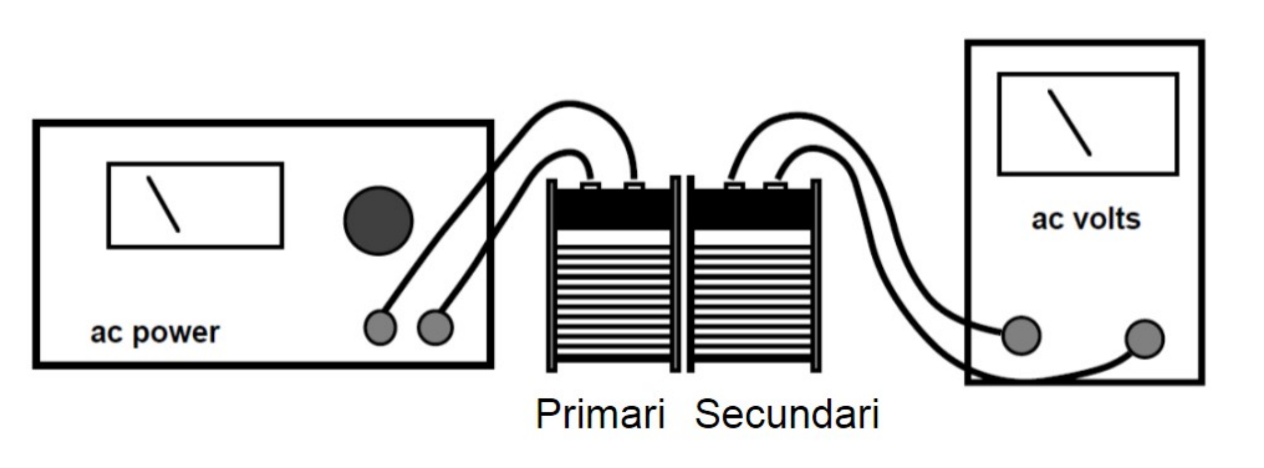
\includegraphics[width=0.38\linewidth]{screenshot007}
	\caption{Esquema de les connexions del transformador}
	\label{fig4:1}
\end{figure}

Com que la font de corrent altern té una escala diferent al voltatge que dóna, els 6 V necessaris es corresponen, teòricament, a la marca 5 de la gradació de l'aparell. A la pràctica usem la marca 6 per ser aquesta més propera al valor de 6 V demanat.

Aquesta part de la pràctica pretén estudiar la variació de la relació entre el voltatge d'entrada i el llegit al secundari segons la configuració en què situem les dues bobines. Així, el procediment sempre serà mesurar el voltage de sortida del transformador i comparar-lo amb el valor d'entrda per tal de determinar amb quina de les configuracions obtenim una lectura de voltatge major.

Inicialment treballem amb dues bobines de 400 voltes. Abans de muntar qualsevol de les configuracions, cal mesurar el voltatge de sortida del transformador.

Tot seguit provem les configuracions que ens proposa el guió de la pràctica que són les representades a la Figura \ref{fig4:2}.

\begin{figure}[h]
	\centering
	\begin{subfigure}[b]{0.22\textwidth}
		\centering
		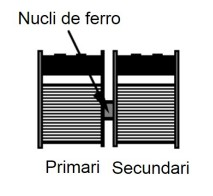
\includegraphics[width=\textwidth]{42a.jpg}
		\caption{Inserció d'una peça petita i recta entre les bobines.}
		\label{fig4:2a}
	\end{subfigure}
	\hspace{0.4cm}
	\begin{subfigure}[b]{0.22\textwidth}
		\centering
		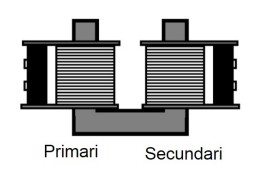
\includegraphics[width=\textwidth]{42b.jpg}
		\caption{Bobines situades als dos costats del nucli en forma d'U.}
		\label{fig4:2b}
	\end{subfigure}
	\hspace{0.4cm}
	\begin{subfigure}[b]{0.22\textwidth}
		\centering
		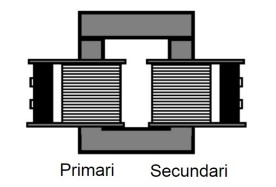
\includegraphics[width=\textwidth]{42c.jpg}
		\caption{Bobines situades als dos costats del nucli amb forma d'U tancat superiorment per la peça recta.}
		\label{fig4:2c}
	\end{subfigure}
	\hspace{0.4cm}
	\begin{subfigure}[b]{0.22\textwidth}
		\centering
		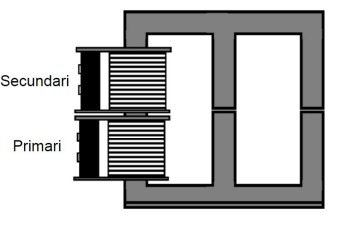
\includegraphics[width=\textwidth]{42d.jpg}
		\caption{Bobines situades a la columna esquerra del nucli.}
		\label{fig4:2d}
	\end{subfigure}
	\caption{Configuracions proposades pel guió.}
	\label{fig4:2}
\end{figure}


Un cop obtenim les lectures de voltatge corresponents, tractem amb altres configuracions que escollim nosaltres. Aquestes es poden veure a la Figura \ref{fig4:3}.

\begin{figure}[h]
	\centering
	\begin{subfigure}[b]{0.3\textwidth}
		\centering
		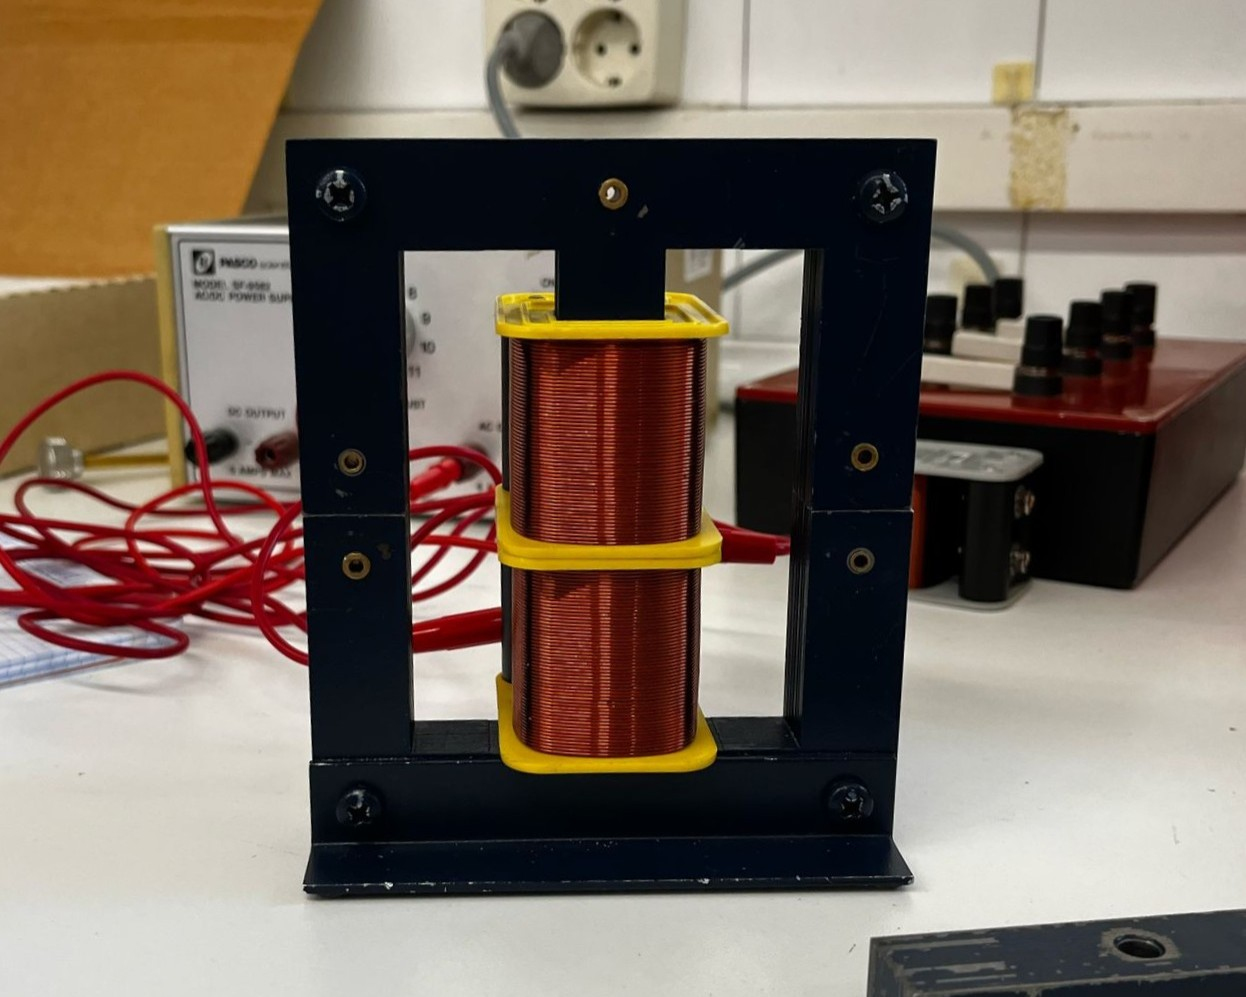
\includegraphics[width=\textwidth]{inv1.jpg}
		\caption{Bobines situades a la columna central del nucli.}
		\label{fig4:3a}
	\end{subfigure}
	\hspace{2cm}
	\begin{subfigure}[b]{0.23\textwidth}
		\centering
		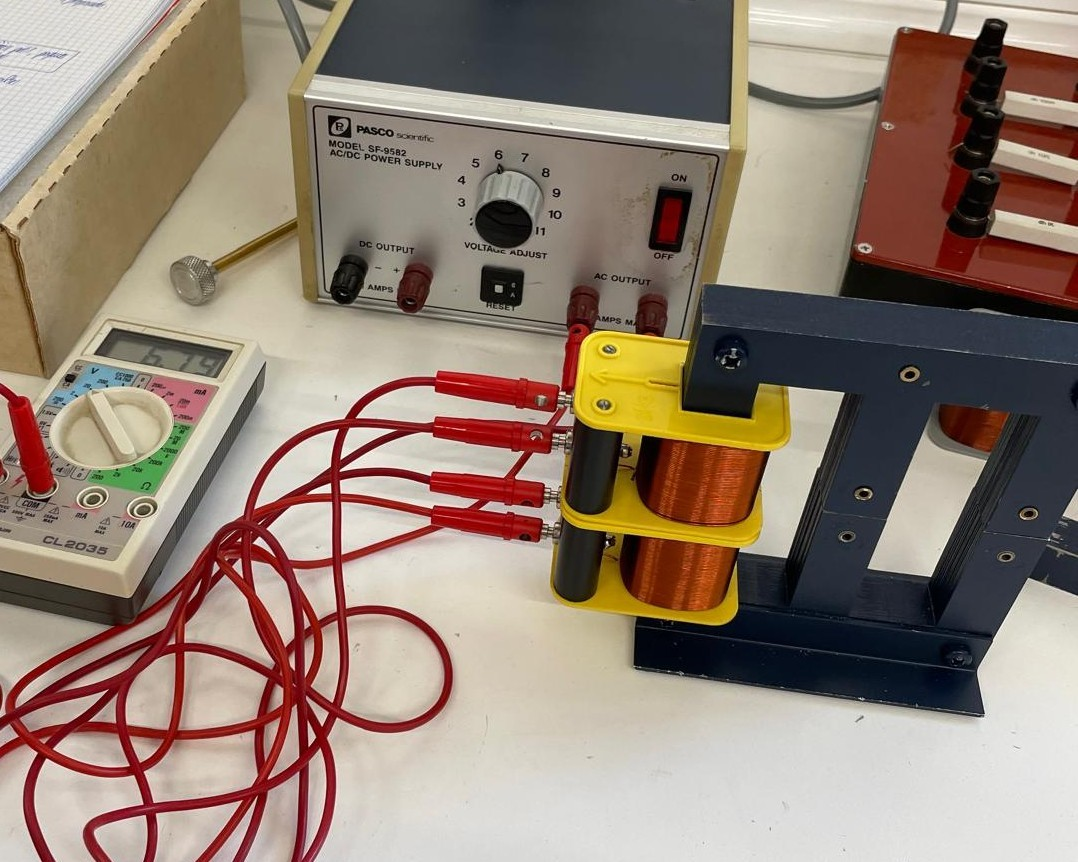
\includegraphics[width=\textwidth]{inv2.jpg}
		\caption{Bobines situades a les columnes esquerra i central del nucli.}
		\label{fig4:3b}
	\end{subfigure}
	\caption{Configuracions triades per nosaltres basades en un nucli format per tres columnes unides tant per la part superior com per la inferior.}
	\label{fig4:3}
\end{figure}


Amb totes les lectures de voltatge, seleccionem aquella configuració que ens dóna un valor més alt. Ara, amb aquesta disposició, provem totes les combinacions possibles de bobines (primaris i secundaris), anotant, de nou, el valor de voltatge del secundari .

\subsection{Estudi de les intensitats i els voltatges d'entrada i de sortida}
Per tal de poder comparar el guany de voltatge teòric i experimental donat per
\begin{equation}
	T_{e/s}=\frac{V_{sortida}}{V_{entrada}}
	\label{eq4:25}
\end{equation}
necessitem trobar la reactància de les bobines amb què treballarem, aquestes són les de 400 i 800 voltes.

La reactància de les bobines es pot calcular muntant el circuit de la Figura \ref{fig4:4} (on $R=1000$ $\Omega$) situant la bobina corresponent al primari i posant el circuit sense connexions a la sortida del transformador, deixant-lo així obert. Mesurant $I_1$ i $V_1$ es calcula la reactància buscada per a cada una de les bobines, usant que
\begin{equation}
	X = \frac{\abs{V}}{\abs{I}}
	\label{eq4:27}
\end{equation}

\begin{figure}[h]
	\centering
	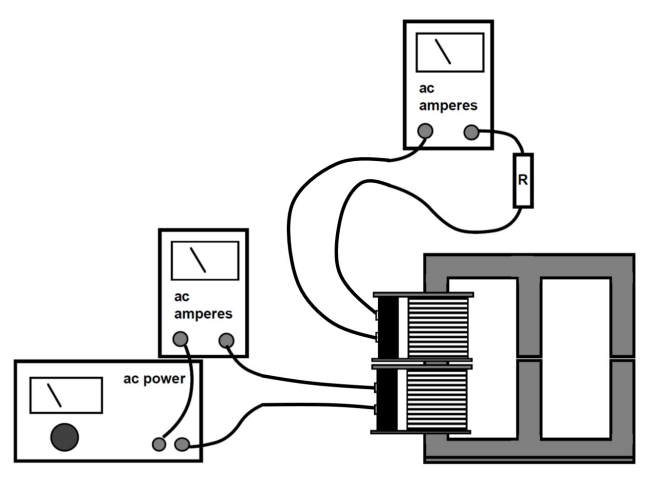
\includegraphics[width=0.4\linewidth]{screenshot010}
	\caption{Muntatge experimental pel càlcul de la reactància de les bobines.}
	\label{fig4:4}
\end{figure}

Un cop obtingut aquest valor, treballem amb el parell de bobines de 400 voltes, situant-ne una al primari i l'altra al secundari. Connectem la resistència de 1000 $\Omega$ i donem un voltatge aproximat de 6 V des de la font d'alimentació. Amb tot això, mesurem el voltatge i el corrent tant d'entrada com de sortida. Aquest mateix procediment es torna a realitzar per les resistències de 10 $\Omega$ i 100 $\Omega$.

Canviem ara la bobina del secundari i la substituïm per una altra de 800 voltes. Realitzant un procediment anàleg a l'anterior, mesurem, de nou, els voltatges i les intensitats d'entrada i de sortida.

\section{Resultats i discussió}
\subsection{Estudi de les variables d'un transformador}
En aquesta secció mesurem els valors experimentals dels voltatges d’entrada i de sortida per a diferents configuracions d’acoblament, utilitzant dues bobines de 400 voltes cadascuna. Cada configuració es correspon a una disposició diferent d’elements ferromagnètics amb diverses geometries. A partir dels voltatges mesurats, calculem els valors de $k$, que es recullen a la taula \ref{tab:4.1}.

\begin{table}[h]
	\centering
	\renewcommand{\arraystretch}{1.2}
	\caption{Valors experimentals dels voltatges d'entrada, $V_1$, dels voltatges de sortida, $V_2$, i de la constant d'acoblament, $k$, per a diferents configuracions del muntatge 400/400.}
	\begin{tabular}{lccc}
		\toprule
		Configuració & $V_1 \,(\mathrm{V})$ & $V_2 \,(\mathrm{V})$ & $k$ \\
		\midrule
		Conf. 0     & 6,20 ± 0,01 & 0,260 ± 0,001 & 0,0419 ± 0,0002 \\
		Conf. a     & 6,82 ± 0,01 & 2,36 ± 0,01   & 0,3460 ± 0,0016 \\
		Conf. b     & 6,97 ± 0,01 & 2,57 ± 0,01   & 0,3687 ± 0,0015 \\
		Conf. c     & 7,05 ± 0,01 & 5,16 ± 0,01   & 0,7319 ± 0,0018 \\
		Conf. d     & 7,07 ± 0,01 & 6,76 ± 0,01   & 0,9562 ± 0,0020 \\
		Conf. proposada 1  & 7,09 ± 0,01 & 6,76 ± 0,01   & 0,9535 ± 0,0020 \\
		Conf. proposada 2  & 7,09 ± 0,01 & 2,93 ± 0,01   & 0,4133 ± 0,0015 \\
		\bottomrule
	\end{tabular}
	\label{tab:4.1}
\end{table}


Podem observar, a partir dels valors de $k$, que la configuració òptima és la d. Aquest resultat és coherent amb la teoria, ja que la presència d’un material ferromagnètic d’alta permeabilitat magnètica afavoreix la concentració i la guia de les línies de camp magnètic, reduint les pèrdues de flux i incrementant el coeficient d’acoblament, acostant-lo al cas ideal ($k = 1$). En aquest cas concret, la geometria del nucli és la més indicada per seguir el recorregut natural del camp creat per la bobina primària, de manera que el flux magnètic queda més confinat i canalitzat cap a la bobina secundària.

Cal destacar que la primera configuració proposada per nosaltres també presenta un valor de $k$ molt proper a la idealitat (0,9535 ± 0,00195), tot i ser lleugerament inferior al de la configuració d (0,9562 ± 0,00196). Malgrat això, considerem que aquesta primera configuració hauria de ser la millor des del punt de vista geomètric, ja que la seva forma s’ajusta especialment bé al recorregut natural de les línies del camp magnètic generades per la bobina primària. Per aquest motiu, l’hem escollida com a base pels càlculs posteriors.

Per finalitzar l'anàlisi, podem veure la importància d’introduir un element ferromagnètic per minimitzar les pèrdues de flux magnètic. Si ens fixem en la configuració 0, que correspon al cas sense cap element ferromagnètic, la constant d’acoblament és de $k = 0,0419 \pm 0,0002 $, el valor més baix amb diferència respecte a la resta de configuracions. Això indica que una gran part del flux magnètic no arriba a la bobina secundària, evidenciant una desviació notable del comportament ideal i una gran pèrdua de voltatge.

Per estudiar com varien els voltatges d'entrada i sortida si canviem les bobines (tan la primària com la secundària), usem la primera configuració proposada (\ref{fig4:2d}) com ja hem comentat anteriorment. Les mesures experimentals dels voltatges d'entrada i de sortida per a les diferents combinacions de bobines es troben a la taula \ref{tab:4.2}. 
\begin{table}[H]
	\centering
	\renewcommand{\arraystretch}{1.2}
	\caption{Valors experimentals dels voltatges d'entrada $(V_1)$ i de sortida $(V_2)$ i la semblança amb la idealitat per a diferents combinacions de bobines (essent $n_1$ i $n_2$ les voltes corresponents a cada bobina) usant la primera configuració proposada per nosaltres.}
	\begin{tabular}{lcccccccc}
		\toprule
		$n_1$ & $n_2$ & $n_2/n_1$ & $V_1 (\text{V})$ & $V_2 (\text{V})$ & $V_2/V_1$ & Idealitat (\%) & Error (\%) \\
		\midrule
		200 & 400 & 2 & $7{,}12 \pm 0{,}01$ & $13{,}89 \pm 0{,}01$ & $1{,}951 \pm 0{,}003$ & 97,54 & 0,15 \\
		200 & 800 & 4 & $7{,}12 \pm 0{,}01$ & $27{,}3 \pm 0{,}1$ & $3{,}834 \pm 0{,}015$ & 95,86 & 0,38 \\
		200 & 1600 & 8 & $7{,}12 \pm 0{,}01$ & $54{,}8 \pm 0{,}1$ & $7{,}697 \pm 0{,}018$ & 96,21 & 0,22 \\
		200 & 3200 & 16 & $7{,}12 \pm 0{,}01$ & $110{,}2 \pm 0{,}1$ & $15{,}478 \pm 0{,}026$ & 96,73 & 0,16 \\
		\midrule
		400 & 200 & 0{,}5 & $7{,}09 \pm 0{,}01$ & $3{,}21 \pm 0{,}01$ & $0{,}453 \pm 0{,}0002$ & 90,55 & 0,31 \\
		400 & 400 & 1 & $7{,}09 \pm 0{,}01$ & $6{,}76 \pm 0{,}01$ & $0{,}953 \pm 0{,}0003$ & 95,35 & 0,19 \\
		400 & 800 & 2 & $7{,}09 \pm 0{,}01$ & $13{,}4 \pm 0{,}01$ & $1{,}882 \pm 0{,}003$ & 94,08 & 0,15 \\
		400 & 1600 & 4 & $7{,}09 \pm 0{,}01$ & $26{,}4 \pm 0{,}01$ & $3{,}724 \pm 0{,}005$ & 93,09 & 0,38 \\
		400 & 3200 & 8 & $7{,}09 \pm 0{,}01$ & $53{,}3 \pm 0{,}01$ & $7{,}516 \pm 0{,}010$ & 93,97 & 0,22 \\
		\midrule
		800 & 200 & 0{,}25 & $7{,}12 \pm 0{,}01$ & $1{,}6 \pm 0{,}01$ & $0{,}2247 \pm 0{,}0003$ & 89,89 & 0,14 \\
		800 & 400 & 0{,}5 & $7{,}12 \pm 0{,}01$ & $3{,}37 \pm 0{,}01$ & $0{,}473 \pm 0{,}001$ & 94,66 & 0,31 \\
		800 & 1600 & 2 & $7{,}12 \pm 0{,}01$ & $13{,}7 \pm 0{,}1$ & $1{,}922 \pm 0{,}015$ & 94,66 & 0,15 \\
		800 & 3200 & 4 & $7{,}12 \pm 0{,}01$ & $27{,}0 \pm 0{,}1$ & $3{,}792 \pm 0{,}015$ & 94,80 & 0,38 \\
		\midrule
		1600 & 200 & 0{,}125 & $7{,}16 \pm 0{,}01$ & $0{,}811 \pm 0{,}001$ & $0{,}1133 \pm 0{,}0002$ & 90,61 & 0,17 \\
		1600 & 400 & 0{,}25 & $7{,}16 \pm 0{,}01$ & $1{,}698 \pm 0{,}01$ & $0{,}2372 \pm 0{,}0003$ & 94,86 & 0,14 \\
		1600 & 800 & 0{,}5 & $7{,}16 \pm 0{,}01$ & $3{,}34 \pm 0{,}01$ & $0{,}4665 \pm 0{,}0015$ & 93,30 & 0,31 \\
		1600 & 1600 & 1 & $7{,}16 \pm 0{,}01$ & $6{,}84 \pm 0{,}01$ & $0{,}955 \pm 0{,}002$ & 93,78 & 0,15 \\
		\midrule
		3200 & 200 & 0{,}0625 & $7{,}09 \pm 0{,}01$ & $0{,}396 \pm 0{,}01$ & $0{,}0559 \pm 0{,}0002$ & 89,37 & 0,26 \\
		3200 & 400 & 0{,}125 & $7{,}09 \pm 0{,}01$ & $0{,}829 \pm 0{,}01$ & $0{,}117 \pm 0{,}0002$ & 93,54 & 0,17 \\
		3200 & 800 & 0{,}25 & $7{,}09 \pm 0{,}01$ & $1{,}669 \pm 0{,}01$ & $0{,}2354 \pm 0{,}0009$ & 94,16 & 0,14 \\
		3200 & 1600 & 0{,}5 & $7{,}09 \pm 0{,}01$ & $3{,}29 \pm 0{,}01$ & $0{,}4640 \pm 0{,}0016$ & 92,81 & 0,31 \\
		\bottomrule
	\end{tabular}
	\label{tab:4.2}
\end{table}

Com veiem en l'equació \eqref{eq:4.transf} del desenvolupament teòric, idealment el guany de voltatge hauria de ser igual a la relació de voltes $\alpha$, per un transformador ideal. L'última columna de la taula mostra el percentatge de semblança entre el valor experimental i el valor teòric ideal. Tot i que cap dels valors és exactament del $100\%$, degut a les pèrdues reals del sistema, podem afirmar que l'equació \eqref{eq:4.transf} es una bona aproximació per a totes les combinacions analitzades. 

Destaquem,  algunes tendències observades. En general, a mesura que augmenta la diferència relativa entre $n_1$ i $n_2$, la desviació respecte del comportament ideal també augmenta. Això pot explicar-se pel fet que les relacions molt desiguals entre les dues bobines afavoreixen les pèrdues per flux dispers i un pitjor acoblament magnètic. D'altra banda, es pot observar que quan el nombre de voltes al primari és molt superior al del secundari, les pèrdues d'inducció sobre el secundari tendeixen a ser més significatives. Això és degut a que es genera un flux magnètic més fort però no sempre ben acoblat, de manera que part d’aquest flux no s’aprofita. En canvi, quan el nombre de voltes al primari és menor o comparable al del secundari, l’eficiència en la transferència de flux tendeix a ser més gran, reduint les pèrdues i acostant-se més al comportament ideal.

Aquestes observacions són coherents amb el comportament esperat per a un transformador real, en el qual les pèrdues per flux dispers, histèresi i escalfament impedeixen que la relació \( \frac{V_2}{V_1} = \frac{n_2}{n_1} \) es compleixi exactament.

\subsection{Estudi de les intensitats i voltatges d'entrada i de sortida}
Comencem buscant la relació entre les reactàncies d'una bobina de 400 voltes i una de 800 voltes a circuit obert. Els valors mesurats experimentalment dels voltatges i corrents d'entrada es poden trobar a la taula \ref{tab:4.3}. 

\begin{table}[H]
	\centering
	\renewcommand{\arraystretch}{1.2}
	\caption{Reactàncies per a bobines de 400 i 800 voltes.}
	\begin{tabular}{lcccc}
		\toprule
		$n$ & $V (\text{V})$ & $I (\text{A})$ & $X(\Omega)$ \\
		\midrule
		400 & $7{,}11 \pm 0{,}01$ & $0{,}0708 \pm 0{,}0001$ & $100{,}42 \pm 0{,}11$ \\
		800 & $7{,}05 \pm 0{,}01$ & $0{,}0183 \pm 0{,}0001$ & $385{,}25 \pm 2{,}17$ \\
		\bottomrule
	\end{tabular}
	\label{tab:4.3}
\end{table}
La reactància de cada bobina la calculem a partir de l'equació trobada a teoria (\ref{eq4:27}).

La inductància ve donada per l'expressió $\ref{eq:4:100}$, és a dir, és proporcional al quadrat del nombre de voltes de la bobina. Com que la reactància és directament proporcional a la inductància, aquesta també serà proporcional al quadrat del nombre de voltes

\begin{equation}
	L \propto n^2, \quad X \propto L \quad \Rightarrow \quad X \propto n^2
\end{equation}

Les constants que intervenen en el valor de la inductància (com la permeabilitat del nucli o les dimensions de la bobina) són comunes a ambdues bobines, ja que tenen la mateixa configuració. Per tant, quan es vol comparar la reactància de dues bobines a circuit obert, la relació entre elles serà igual al quadrat del quocient del nombre de voltes de cada bobina

\begin{equation}
	\frac{X_{800}}{X_{400}} = \left( \frac{800}{400} \right)^2 = 4. \label{eq:4.30}
\end{equation}


La relació ens dona un valor de $ 3,84 \pm 0,02 $. 

Aquest valor és coherent amb el valor teòric esperat de 4, confirmant que la reactància és proporcional al quadrat del nombre de voltes de la bobina. 

Per a segona part d'aquesta secció, connectem un circuit al secundari, sempre amb una bobina de 400 voltes, i estudiem els corrents d’entrada i de sortida. A la taula \ref{tab:4.4} es mostren les mesures experimentals dels voltatges i les intensitats d'entrada i sortida per a les combinacions amb 400 i 800 voltes al primari, i una combinació proposada per nosaltres amb 3200 voltes. La configuració usada és la que es demana al guió, que és la \textbf{d} (\ref{fig4:2d}). 

\begin{table}[H]
	\centering
	\renewcommand{\arraystretch}{1.2}
	\caption{Valors experimentals del guany en voltatge a partir de les mesures experimentals dels voltatges i corrents per a diferents combinacions de bobines usant la configuració \textbf{d} (\ref{fig4:2d}).}
	\begin{tabular}{lccccccc}
		\toprule
		$n_1/n_2$ & $\alpha$ & $R\,(\Omega)$ & $V_1$ (V) & $I_1$ (A) & $V_2$ (V) & $I_2$ (A) & $V_2/V_1$ \\
		\midrule
		& & 1000 & $7{,}31 \pm 0{,}01$ & $0{,}0489 \pm 0{,}0001$ & $7{,}00 \pm 0{,}01$ & $0{,}0064 \pm 0{,}0001$ & $0{,}9576 \pm 0{,}0019$ \\
		$400/400$ & 1 & 100  & $7{,}28 \pm 0{,}01$ & $0{,}0778 \pm 0{,}0001$ & $6{,}70 \pm 0{,}01$ & $0{,}0515 \pm 0{,}0001$ & $0{,}9203 \pm 0{,}0019$  \\
		& & 10   & $7{,}17 \pm 0{,}01$ & $0{,}1862 \pm 0{,}0001$ & $4{,}31 \pm 0{,}01$ & $0{,}1703 \pm 0{,}0001$ & $0{,}6011 \pm 0{,}0016$\\
		\midrule
		& & 1000 & $7{,}16 \pm 0{,}01$ & $0{,}0587 \pm 0{,}0001$ & $13{,}45 \pm 0{,}01$ & $0{,}0119 \pm 0{,}0001$ & $1{,}878 \pm 0{,}003$  \\
		$800/400$ & 0{,}5 & 100  & $7{,}10 \pm 0{,}01$ & $0{,}1585 \pm 0{,}0005$ & $11{,}07 \pm 0{,}01$ & $0{,}0712 \pm 0{,}0005$ & $1{,}559 \pm 0{,}003$ \\
		& & 10   & $7{,}03 \pm 0{,}01$ & $0{,}62 \pm 0{,}01$ & $3{,}06 \pm 0{,}01$ & $0{,}29 \pm 0{,}01$ & $0{,}4353 \pm 0{,}0016$ \\
		\midrule
		& & 1000 & $7{,}21 \pm 0{,}01$ & $0{,}32 \pm 0{,}01$ & $39{,}2 \pm 0{,}1$ & $0{,}0385 \pm 0{,}0001$ & $5{,}437 \pm 0{,}016$ \\
		$3200/400$ & 0{,}125 & 100  & $7{,}16 \pm 0{,}01$ & $0{,}66 \pm 0{,}01$ & $8{,}64 \pm 0{,}01$ & $0{,}0811 \pm 0{,}0001$ & $1{,}207 \pm 0{,}002$  \\
		& & 10   & $7{,}17 \pm 0{,}01$ & $0{,}72 \pm 0{,}01$ & $0{,}95 \pm 0{,}01$ & $0{,}0890 \pm 0{,}0001$ & $0{,}1325 \pm 0{,}0014$ \\
		\bottomrule
	\end{tabular}
	\label{tab:4.4}
\end{table}

Un cop calculat el guany $\frac{V_2}{V_1}$, el comparem amb el valor teòric. La  taula \ref{tab:4.5} presenta els valors experimentals i teòrics calculats tenint en compte en quin cas dels tres presentats a la introducció teòrica ens trobem ($Z \gg X$, $Z \sim X$, $Z\ll X$). També es troba l'error respecte el valor teòric.  

\begin{table}[H]
	\centering
	\renewcommand{\arraystretch}{1.2}
	\caption{Taula de comparació entre el guany experimental i el guany teòric, acompanyat de l'error (\%) i les seves incerteses.}
	\begin{tabular}{llccccc}
		\toprule
		$n_1/n_2$ & $Z$ ($\Omega$) & Cas & $X$ ($\Omega$) & $V_2/V_1$ exp & $V_2/V_1$ teòric & Error (\%) \\
		\midrule
		400/400 & 1000 & $Z \gg X$ & 100,42 & 0,9576 $\pm$ 0,0019 & 0,956 $\pm$ 0,002 & 0,15 \\
		& 100  & $Z \sim X$ & 100,42 & 0,9203 $\pm$ 0,0019 & 0,956 $\pm$ 0,002 & 3,75 \\
		& 10   & $Z \ll X$ & 100,42 & 0,6011 $\pm$ 0,0016 & 0,724 $\pm$ 0,015 & 17,03 \\
		\midrule
		800/400 & 1000 & $Z \gg X$ & 385,2 & 1,878 $\pm$ 0,003 & 0,4781 $\pm$ 0,0016 & 292,93 \\
		& 100  & $Z \sim X$ & 385,2 & 1,559 $\pm$ 0,003 & 0,4781 $\pm$ 0,0016 & 226,13 \\
		& 10   & $Z \ll X$ & 385,2 & 0,4353 $\pm$ 0,0016 & 0,369 $\pm$ 0,011 & 18,10 \\
		\midrule
		3200/400 & 1000 & $Z \sim X$ & 6295,5 & 5,437 $\pm$ 0,016 & 0,1195 $\pm$ 0,0004 & 4448,97 \\
		& 100  & $Z \ll X$ & 6295,5 & 1,207 $\pm$ 0,002 & 0,1191 $\pm$ 0,0004 & 913,22 \\
		& 10   & $Z \ll X$ & 6295,5 & 0,1325 $\pm$ 0,0014 & 0,091 $\pm$ 0,003 & 45,04 \\
		\bottomrule
	\end{tabular}
	\label{tab:4.5}
\end{table}



Abans de comentar els resultats, cal fer una observació sobre la reactància corresponent a la bobina de 3200 voltes, la combinació proposada per nosaltres. Les reactàncies de les altres dues bobines s'han obtingut a partir de mesures experimentals de la primera part d'aquesta secció. En canvi, com que no vam mesurar experimentalment la reactància de la bobina de 3200 voltes, hem hagut de recórrer a la teoria que acabem de demostrar a l'apartat anterior per poder estimar-la. A partir d'això podem establir una relació entre la reactància de la bobina de 3200 voltes i les reactàncies de les bobines de 800 i 400 voltes (d'una forma molt similar al que es té en l'equació \eqref{eq:4.30}), de manera que
\begin{align*}
	X_{3200}  &= \left(\frac{3200}{800}\right)^2 X_{800} = 16 X_{800},  \\
	X_{3200}  &= \left(\frac{3200}{400}\right)^2 X_{400} = 64 X_{400}. 
\end{align*}
Fent la mitjana entre els dos valors obtinguts, tenim que 

\begin{equation}
	X_{3200} = 6295,5 \text{ $\Omega$}
\end{equation}


\textcolor{red}{VALE AQUI HAURIA DE COMENTAR ALGO LOKA (ERRORS???????????????????)}

Un cop analitzades les diferents configuracions, ens fixem ara en com petites variacions en el coeficient d’acoblament $k$ poden afectar el guany. Per fer-ho, considerem una disminució de $\Delta k = 0{,}0062$, tenint doncs, un valor de $k' = 0,9500$, i calculem la variació relativa del guany teòric mantenint la resta de paràmetres constants. Els resultats es recullen a la taula \ref{tab:4.6}.


\begin{table}[H]
	\centering
	\renewcommand{\arraystretch}{1.2}
	\caption{Variació del guany teòric per un petit canvi en $k$.}
	\begin{tabular}{llcccccc}
		\toprule
		$n_1/n_2$ & $Z$ ($\Omega$) & Cas & $k$ & $V_2/V_1$ amb $k$ & $k'$ & $V_2/V_1$ amb $k'$ & Variació relativa del guany (\%) \\
		\midrule
		400/400 & 1000 & $Z \gg X$ & 0,9562 & 0,95615 & 0,9500 & 0,9500 & 0,64 \\
		& 100  & $Z \sim X$ & 0,9562 & 0,95615 & 0,9500 & 0,9500 & 0,64 \\
		& 10   & $Z \ll X$ & 0,9562 & 0,72446 & 0,9500 & 0,6788 & 6,30 \\
		\midrule
		800/400 & 1000 & $Z \gg X$ & 0,9562 & 0,47808 & 0,9500 & 0,4750 & 0,64 \\
		& 100  & $Z \sim X$ & 0,9562 & 0,47808 & 0,9500 & 0,4750 & 0,64 \\
		& 10   & $Z \ll X$ & 0,9562 & 0,36858 & 0,9500 & 0,3463 & 6,05 \\
		\midrule
		3200/400 & 1000 & $Z \sim X$ & 0,9562 & 0,11952 & 0,9500 & 0,1188 & 0,64 \\
		& 100  & $Z \ll X$ & 0,9562 & 0,11910 & 0,9500 & 0,1182 & 0,75 \\
		& 10   & $Z \ll X$ & 0,9562 & 0,09135 & 0,9500 & 0,0857 & 6,18 \\
		\bottomrule
	\end{tabular}
	\label{tab:4.6}
\end{table}

A partir de les dades de la taula, observem que una petita variació de $k$  pot provocar una variació relativa del guany superior al $6\,\%$, però aquest efecte només es manifesta clarament en les configuracions on la impedància de càrrega és molt petita ($Z \ll X$). En la resta de casos, la variació és pràcticament negligible.

Cal mencionar que, tot i que les dues configuracions amb $3200/400$ voltes i resistències de $100\,\Omega$ i $10\,\Omega$ pertanyen al mateix règim ($Z \ll X$), només en el cas de $10\,\Omega$ el guany teòric mostra una dependència clara amb $k$. Aquest comportament es pot explicar analitzant l’expressió del guany (equació~\ref{eq4:22}), on apareix un terme amb $k$ en el denominador
\begin{equation*}
	\sqrt{Z^2 + X^2 \alpha^4 (k^2 - 1)^2}.
\end{equation*}
En aquestes dues configuracions, la reactància $X = 6295,5$ $\Omega$ i la relació de voltes $\alpha = 0{,}125$ es mantenen constants, de forma que l’únic paràmetre que canvia és la impedància $Z$, que és igual, en aquest experiment, a la resistència aplicada al secundari, $R$, per tant, $Z =R $. Si comparem els quadrats de les impedàncies, obtenim $Z^2 = 100$ per al cas de 10 $\Omega$ i $Z^2 = 10000$ per al cas de 100 $\Omega$.

En el primer cas ($Z = 10$ $\Omega$), el valor de $Z^2$ és del mateix ordre de magnitud que el terme en $k$, de manera que aquest últim té un pes significatiu en el denominador i el guany passa a dependre clarament del valor de $k$. En canvi, en el segon cas ($Z=10$ $\Omega$), el terme $Z^2$ domina clarament al denominador, fent que la contribució del terme amb $k$ sigui negligible. Aquesta és, doncs, l’excepció que no segueix la tendència observada.

De fet, a mesura que el nombre de voltes del primari augmenta respecte del secundari, el quocient $\alpha$ es fa molt petit, i en conseqüència $\alpha^4$ es fa gairebé nul. Tot i que la reactància $X$ també augmenta (ja que, com hem vist $X \propto n_1^2$ REF), aquest creixement no és suficient per compensar la pèrdua deguda a $\alpha^4$ dins el terme $X^2 \alpha^4 (k^2 - 1)^2$, que esdevé totalment negligible. A més a més, aquest augment de $X$ permet fer servir resistències relativament grans i continuar estant dins el règim $Z \ll X$. Això fa que el terme $Z^2$ del denominador domini completament i anul·li l’efecte de $k$, independentment de la seva variació. En resum, com més gran és la diferència entre el nombre de voltes del primari i del secundari, més fàcil és que el coeficient d’acoblament $k$ deixi de tenir impacte en el guany.

Per contra, si ens fixem ens els altres casos, $Z \gg X$ (\ref{eq4:20}) o $Z \sim X$ (\ref{eq4:24}), el guany té una dependència lineal en $k$ , i per tant, petites variacions en aquest coeficient només provoquen canvis mínims en el guany teòric. Això explica per què els percentatges de variació són molt menors en aquests casos.



\section{Conclusions}
En aquesta pràctica hem pogut constatar la importància d'incorporar un nucli ferromagnètic en un transformador per tal de minimitzar les pèrdues de flux magnètic. Per analitzar aquest efecte, s’han muntat diferents configuracions amb diverses geometries pel nucli, i s’ha determinat que la configuració òptima és la que segueix millor les línies de camp generades per les bobines, ja que presenta una millor canalització del flux magnètic i, per tant, un coeficient d’acoblament més proper a la idealitat ($k = 1$).

A continuació, hem estudiat diferents combinacions del nombre de voltes al primari i secundari, mantenint constant la resta de paràmetres, per comprovar la llei que relaciona els voltatges d'entrada i de sortida en funció de les característiques de les bobines. Tot i que els resultats obtinguts mostren valors de guany propers a la idealitat, s’ha observat que, a mesura que augmenta la diferència entre el nombre de voltes del primari i del secundari, i sent $n1$ major a $n2$, el comportament del transformador s’allunya més del model ideal. Aquesta desigualtat afavoreix les pèrdues de flux i redueix l’eficiència de l’acoblament magnètic.

En la segona part de la pràctica, hem demostrat la relació entre les reactàncies de dues bobines en circuit obert i s’ha utilitzat aquesta expressió per estimar la reactància d’una bobina amb 3200 voltes que no es va mesurar experimentalment, però que era necessària per a les anàlisis posteriors.

Finalment, hem comparat el guany en voltatge experimental amb el teòric, per diferents valors de la relació $n_2/n_1$ i per diferents resistències. Per calcular el guany en voltatge teòric, s'ha tingut en compte en quin règim ens trobem ($Z \gg X$, $Z \sim X$ i $Z \ll X$). En cada cas, s’han aplicat les aproximacions teòriques corresponents, i hem observat que, en el règim $Z \ll X$, la dependència del guany respecte el coeficient d’acoblament $k$ és molt més significativa que en la resta.


\begin{thebibliography}{99}
	\bibitem{ref1}
	\textit{Col·lecció de problemes de l'assignatura d'Electromagnetisme.}
	
	\bibitem{ref2}
	\textit{World Magnetic Model 2025 Calculator}, Natural Environment Research Council. Consultat el: 17/03/2025.\\ 
	\url{http://www.geomag.bgs.ac.uk/data_service/models_compass/wmm_calc.html}.
	
	\bibitem{ref3}
	\textit{Guions de les pràctiques de l'assignatura de Laboratori d'Electromagnetisme}.
\end{thebibliography}

\newpage
\begin{appendices}
%SI TOQUEU AIXÒ ELS ANNEXOS PETEN.

\textbf{\Huge{Annexos}}
\renewcommand{\thesection}{\Alph{section}} % Cambia la numeración de capítulos a letras
\renewcommand{\theequation}{\thesection.\arabic{equation}} % Cambia numeración de ecuaciones
\setcounter{equation}{0} % Reinicia contador de ecuaciones en cada sección

\section{Càlcul d'incerteses}
\label{an:a3}
Pel càlcul de les incerteses associades a cada pràctica s'ha utilitzat la llei de propagació d'incerteses
\begin{equation}
	u_F = \sqrt{ \left( \frac{\partial F}{\partial x_1} \right)^2 u_{x_1}^2 + \left( \frac{\partial F}{\partial x_2} \right)^2 u_{x_2}^2 + \dots + \left( \frac{\partial F}{\partial x_n} \right)^2 u_{x_n}^2 },
\end{equation}
on $F(x_1,x_2,\ldots,x_n)$ és la funció considerada i $u_i$ la incertesa associada a cada $x_i$.

Per aquells casos on és necessari tenir en compte incerteses estadístiques, aquestes es calculen segons
\begin{equation}
	u_X=\frac{s_X}{\sqrt{N}}
\end{equation}
sent $s_X$ la desviació estàndard de la mostra i $N$ el nombre de mesures efectuades.

Finalment, per la incertesa combinada s'utilitza
\begin{equation}
	u_C=\sqrt{u_{instrumental}^2+u_{estadistica}^2}.
\end{equation}

\subsection{Incerteses de la pràctica 1}
Per simplicitat anomenem $\frac{\Delta V_i \Delta l_i}{\Delta r_i} = Y_i$, de forma que:
\begin{enumerate}
	\item Paràmetre Y$_i$: \begin{equation}
		u_{Y_i} = \sqrt{ \left( \frac{\Delta l_i \Delta V_i}{\Delta r_i} u_{\Delta V_i} \right)^2 + \left( \frac{\Delta V_i \Delta l_i}{\Delta r_i} u_{\Delta l_i} \right)^2 + \left( \frac{\Delta l_i \Delta V_i}{\Delta r_i^2} u_{\Delta r_i} \right)^2 }.
	\end{equation}
	\item Càrrega per unitat de longitud:\begin{equation}
		\frac{Q}{Z} = \varepsilon \sum_i Y_i \implies u_{Q/Z} = \varepsilon \sqrt{\sum_i u_{Y_i}^2}.
	\end{equation}
	\item Capacitat per unitat de longitud:\begin{equation}
		u_{\frac{C}{Z}} = \sqrt{ \left( \frac{1}{Z \, \Delta V} u_Q \right)^2 + \left( \frac{Q}{Z \, \Delta V^2} u_{\Delta V} \right)^2 }.
	\end{equation}
	\item Capacitat teòrica\begin{equation}
		u_{C_\text{teòrica}} = \frac{u_H}{d} \sqrt{1+C^2}.
	\end{equation}
\end{enumerate}
\subsection{Incerteses de la pràctica 2}
\begin{enumerate}
	\item Força segons la segona llei de Newton: \begin{equation}
		u_F=\sqrt{m^2u_g^2+g^2u_m^2}.
	\end{equation}
	\item Mitjana de les mesures de la intensitat (incertesa estadística): \begin{equation}
		u_{estad. I}= \frac{s_I}{\sqrt{3}}.
	\end{equation}
	\item Intensitat: \begin{equation}
		u_I=\sqrt{u_{instr. I}^2+u_{estad. I}^2}.
	\end{equation}
	\item Intensitat al quadrat: \begin{equation}
		u_{I^2}=2Iu_I.
	\end{equation}
	\item $\mu_0$ experimental ($I^2$ vs. $F$):

	Definim el pendent de la representació de la intensitat al quadrat en funció de la força amb un paràmetre $A$ tal que:
	\begin{equation*}
		A\equiv\frac{2\pi r}{\mu_0L}.
	\end{equation*}
	Amb això, la incertesa és
	\begin{equation}
		u_{\mu_0}=\sqrt{\left(\frac{2\pi u_r}{LA}\right)^2+\left(\frac{2\pi r u_L}{L^2A}\right)^2+\left(\frac{2\pi ru_A}{LA^2}\right)^2}.
	\end{equation}
	$u_A$ s'obté a partir dels paràmetres de la recta representada.
	\item Angle en radiants: \begin{equation}
		u_{\theta}=\frac{u_{graus}2\pi}{360}.
	\end{equation}
	\item Inversa de la distància: \begin{equation}
		u_{1/r}=\frac{u_r}{r^2}.
	\end{equation}
	\item $\mu_0$ experimental ($F$ vs. $1/r$):
	
	Definim el pendent de la representació de la força en funció de l'invers de la distància amb un paràmetre D tal que: \begin{equation*}
		D\equiv\frac{\mu_0I^2L}{2\pi}.
	\end{equation*}
	Amb això, la incertesa és
	\begin{equation}
		u_{\mu_0}=\sqrt{\left(\frac{2\pi u_D}{I^2L}\right)^2+\left(\frac{4\pi Du_I}{I^3L}\right)^2+\left(\frac{2\pi D u_L}{I^2L}\right)^2}.
	\end{equation}
	\item Força calculada a partir de $F=k\theta$: \begin{equation}
		u_F=\sqrt{k^2u_{\theta}^2+\theta^2u_{k}^2}.
	\end{equation}
	\item Camp d'inducció magnètica: \begin{equation}
		u_B=\sqrt{\left(\frac{u_F}{IL}\right)^2+\left(\frac{Fu_I}{I^2L}\right)^2+\left(\frac{Iu_L}{IL^2}\right)^2}.
	\end{equation}
	\item Camp d'inducció magnètica mitjà (6 mesures): \begin{equation}
		u_{estad.B}=\frac{s_B}{\sqrt{6}}.
	\end{equation}
\end{enumerate}
\subsection{Incerteses de la pràctica 3}
\begin{enumerate}
	\item Freqüència de ressonància teòrica: \begin{equation}
		u_{f_0}=\pi f_0^2\sqrt{\frac{C}{L}u_L^2+\frac{L}{C}u_C^2}.
	\end{equation}
	\item Freqüència angular teòrica: \begin{equation}
		u_{\omega_0}=\frac{1}{2}\omega_0^2\sqrt{\frac{C}{L}u_L^2+\frac{L}{C}u_C^2}.
	\end{equation}
	\item Percentatge d'error entre el valor teòric $T$ i l'experimental $E$: \begin{equation}
		u_{Error}=100\sqrt{\left(\frac{E}{T^2}u_T\right)^2+\left(\frac{u_E}{T}\right)^2}.
	\end{equation}
	\item Guany de voltatge a la resistència: \begin{equation}
		\begin{aligned}
			u_{T_R} = \bigg[ &
			\left( \frac{T_R}{R} (1 - T_R^2) \, u_R \right)^2 + 
			\left( -\frac{T_R^3}{R^2} \left( L\omega^2 - \frac{1}{C} \right) u_L \right)^2 + \\
			& +\left( -\frac{T_R^3}{R^2} \left( L\omega - \frac{1}{C\omega} \left( \frac{1}{C^2 \omega}\right) \right) u_C \right)^2 + 
			\left( -\frac{T_R^3}{R^2} \left( L\omega - \frac{1}{C\omega} \left( L + \frac{1}{C\omega^2} \right) \right) u_{\omega} \right)^2 
			\bigg]^{1/2}.
		\end{aligned}
	\end{equation}
\end{enumerate}
\subsection{Incerteses de la pràctica 4}
\begin{enumerate}
	\item Coeficient d'acoblament: \begin{equation}
		u_k=\sqrt{\left(\frac{1}{V_1\alpha}u_{V_2}\right)^2+\left(\frac{V_2}{V_1^2\alpha}u_{V_1}\right)^2}.
	\end{equation}
	\item Guany de voltatge: \begin{equation}
		u_{\frac{V_2}{V_1}}=\alpha u_k.
	\end{equation}
	\item Reactància 1: \begin{equation}
		u_{X_1}=\sqrt{\left(\frac{1}{I_1}u_{V_1}\right)^2+\left(\frac{V_1}{I_1^2}u_{I_1}\right)^2}.
	\end{equation}
	\item Relació entre la reactància de cada bobina $\left(X_2/X_1\right)$: \begin{equation}
		u_{\frac{X_2}{X_1}}=\sqrt{\left(\frac{1}{X_1}u_{X_2}\right)^2+\left(\frac{X_2}{X_1^2}u_{X_1}\right)^2}.
	\end{equation}
	\item Guany de voltatge pel cas $Z\ll X$: 
	\begin{equation}
		\small
		u_{\frac{V_2}{V_1}}=\sqrt{\left(\frac{\alpha Z\left(Z^2+X^2\alpha^4\left(k^2-1\right)^2\right)-2k^2X^2\alpha^5\left(k^2-1\right)Z}{\left(Z^2+X^2\alpha^4\left(k^2-1\right)^2\right)^{3/2}}u_k\right)^2+\left(\frac{X\alpha^5kZ\left(k^2-1\right)^2}{\left(Z^2+X^2\alpha^4\left(k^2-1\right)^2\right)^{3/2}}u_X\right)^{2}}.
	\end{equation}
\end{enumerate}
\newpage
\section{Annex pràctica 1. Representació de camps}
\subsection{Deducció de l'equació $(1.22)$}
\label{an:a1}
Per deduir l'expressió donada per l'equació \eqref{eqsuppon} ens basarem ens els resultats del problema 2.18 de la llista de problemes de l'assignatura \cite{ref1}. Suposem dos fils infinits rectilinis i carregats amb densitat de càrrega uniforme $\lambda$ i -$\lambda$ separats per una distància $d=2a$. Siguin $\rho_1$ i $\rho_2$ les distàncies radials de cada fil al punt en el qual volem calcular el camp i el potencial. Per la simetria del sistema podem assegurar que $\vec{E}(\vec{r}) = E(\rho) \vec{e}_{\rho}$, de forma que podem aplicar el teorema de Gauss com se segueix:

\[
\left.
\begin{array}{c}
	\oint \vec{E} \cdot \mathrm{d}\vec{S} = E 2\pi \rho L \\[10pt]
	\frac{Q_{int}}{\varepsilon_0} = \frac{1}{\varepsilon_0} \int \lambda \, \mathrm{d}l = \frac{\lambda}{\varepsilon_0} L
\end{array}
\right\}
\quad \Rightarrow \quad 
\vec{E} = \frac{\lambda}{2\pi \varepsilon_0} \frac{1}{\rho} \vec{e}_{\rho}.
\]

Així, essent $\vec{E_1}$ el camp associat al fil amb densitat $\lambda$ i $\vec{E_2}$ el camp associat al fil amb densitat -$\lambda$, tenim:
\begin{align}
	\vec{E_1} & = \frac{\lambda}{2\pi \varepsilon_0} \frac{1}{\rho_1} \vec{e}_{\rho_1}, \\
	\vec{E_2} & = -\frac{\lambda}{2\pi \varepsilon_0} \frac{1}{\rho_2} \hat{e}_{\rho_2},
\end{align}
on:
\begin{align}
	\rho_1 & = \sqrt{(x-a)^2+y^2}, \\
	\rho_2 & = \sqrt{(x+a)^2+y^2}. 
\end{align}
Si calculem el camp usant que
\begin{equation}
	\phi(r) = -\int_{\vec{r}_{ref}}^{\vec{r}}\vec{E}(\vec{r})\cdot \mathrm{d}\vec{r} ,
\end{equation}
i aplicant el principi de superposició, és a dir
\begin{equation}
	\phi = \phi_1+\phi_2,
\end{equation}
trobem que, el potencial generat per aquesta distribució de càrrega obeeix la següent equació:
\begin{equation}
	\phi = \frac{\lambda}{2\pi \varepsilon_0}\ln\sqrt{\frac{(x+a)^2+y^2}{(x-a)^2+y^2}}.
\end{equation}
Les superfícies equipotencials seran aquelles regions de l'espai en què el potencial sigui constant. Escollint
\begin{equation}
	k \equiv e^{\frac{\phi2\pi\varepsilon_0}{\lambda}} = \sqrt{\frac{(x+a)^2+y^2}{(x-a)^2+y^2}},
\end{equation}
i reescrivint segons
\begin{equation}
	k^2[(x-a)^2+y^2]=(x+a)^2+y^2,
\end{equation}  
podem desenvolupar fins a arribar a
\begin{equation}
	\boxed{y^2+\left( x+a\frac{1+k^2}{1-k^2}\right)^2 = a^2\left( \frac{2k}{1-k^2}\right)^2},
\end{equation}
que és l'equació per les superfícies (línies) equipotencials.

\newpage
\subsection{Expressió analítica de la distribució de dos plans secants i un fil}
\label{an:a6}
Per obtenir les expressions analítiques apliquem la definició del potencial i integrem
\begin{equation}
	\phi (x,y) = \frac{1}{4\pi\varepsilon}\int_S\frac{\sigma(x',y')}{\sqrt{(x-x')^2+(y-y')^2}}\mathrm{d}s'.
\end{equation}
Les coordenades prima son les referents a la distribució de carrega i $S$ tota la regió on hi hagi càrrega. Separarem la distribució en tres parts: la càrrega puntual, la part de la placa inferior i la superior, finalment apliquem el principi de superposició per conèixer el potencial que crea la nostra distribució. El potencial que crea la càrrega puntual a la posició $\vec{r_q}$ és:
\begin{equation}
	\phi_q (x,y) = -\frac{1}{4\pi\varepsilon}\frac{q}{\sqrt{(x-d)^2+y^2}}.
\end{equation}
Per resoldre la integral per les plaques hem de tenir en compte que és una distribució unidimensional de càrrega, de manera que $\sigma(x',y') \rightarrow \lambda(x',y')$ i $\mathrm{d}s' \rightarrow \mathrm{d}L$. Per la geometria del problema podem veure que $y' = \tan(\pi/6)x'$ per la placa superior i $y' = -\tan(\pi/6)x'$ per la inferior, de forma que $\phi_{sup}(x,y) = \phi_{inf}(x,-y)$. Per tant:
\begin{align}
	\phi_{sup}(x,y)&=\frac{1}{4\pi\varepsilon}\int_{0}^{\frac{\sqrt{3}}{2}L} \frac{q/L}{\sqrt{(x-x')^2+(y-\frac{\sqrt{3}}{2}x')^2}}\mathrm{d}x', \\
	\phi_{sup}(x,y)&=\frac{1}{4\pi\varepsilon}\frac{\sqrt{3}}{2}\ln \left[\frac{\frac{4}{\sqrt{3}}\sqrt{(x^2+y^2)+L(-\sqrt{3}x+y+L)}+\frac{2}{3}(-3x+\sqrt{3}y+2\sqrt{3}L)}{\frac{4}{\sqrt{3}}\sqrt{x^2+y^2}-\frac{2}{3}(3x-\sqrt{3}y)}\right].
\end{align}
Finalment, podem trobar el potencial total segons:
\begin{equation}
	\phi(x,y) = \phi_q(x,y) + \phi_{sup}(x,y) + \phi_{sup}(x,-y). \\
\end{equation}
El camp elèctric, per la seva banda, serà:
\begin{equation}
	\vec{E}(x,y) = -\vec{\nabla}\phi(x,y).
\end{equation}
\newpage
\subsection{Dades experimentals de la pràctica 1}
\label{an:a2}
A continuació mostrem els valors experimentals obtinguts en el transcurs de la pràctica 1.
\begin{table}[h]
	\centering
	\renewcommand{\arraystretch}{1.2}
	\caption{Valors experimentals mesurats per tal de poder calcular la capacitat del condensador de plaques planoparal·leles.}
	\begin{tabular}{cccc}
		\toprule
		$\Delta l_i$ (m) & $\Delta r_i$ (m) & $\Delta V_i$ (V) & $\frac{\Delta V_i\Delta l_i}{\Delta r_i}$ (V)\\
		\midrule
		0,005 $\pm$ 0,001 & 0,019 $\pm$ 0,001 & 1,00 $\pm$ 0,01 & 0,26 $\pm$ 0,23 \\
		0,005 $\pm$ 0,001 & 0,024 $\pm$ 0,001 & 1,00 $\pm$ 0,01 & 0,21 $\pm$ 0,20 \\
		0,010 $\pm$ 0,001 & 0,038 $\pm$ 0,001 & 1,00 $\pm$ 0,01 & 0,26 $\pm$ 0,16 \\
		0,010 $\pm$ 0,001 & 0,050 $\pm$ 0,001 & 1,00 $\pm$ 0,01 & 0,20 $\pm$ 0,14 \\
		0,005 $\pm$ 0,001 & 0,057 $\pm$ 0,001 & 1,00 $\pm$ 0,01 & 0,09 $\pm$ 0,13 \\
		0,005 $\pm$ 0,001 & 0,063 $\pm$ 0,001 & 1,00 $\pm$ 0,01 & 0,08 $\pm$ 0,13 \\
		0,010 $\pm$ 0,001 & 0,070 $\pm$ 0,001 & 1,00 $\pm$ 0,01 & 0,14 $\pm$ 0,12 \\
		0,005 $\pm$ 0,001 & 0,071 $\pm$ 0,001 & 1,00 $\pm$ 0,01 & 0,07 $\pm$ 0,12 \\
		0,009 $\pm$ 0,001 & 0,066 $\pm$ 0,001 & 1,00 $\pm$ 0,01 & 0,14 $\pm$ 0,12 \\
		0,010 $\pm$ 0,001 & 0,034 $\pm$ 0,001 & 1,00 $\pm$ 0,01 & 0,29 $\pm$ 0,17 \\
		0,008 $\pm$ 0,001 & 0,024 $\pm$ 0,001 & 1,00 $\pm$ 0,01 & 0,33 $\pm$ 0,20 \\
		0,005 $\pm$ 0,001 & 0,014 $\pm$ 0,001 & 1,00 $\pm$ 0,01 & 0,36 $\pm$ 0,27 \\
		0,005 $\pm$ 0,001 & 0,009 $\pm$ 0,001 & 1,00 $\pm$ 0,01 & 0,56 $\pm$ 0,34 \\
		0,002 $\pm$ 0,001 & 0,004 $\pm$ 0,001 & 1,00 $\pm$ 0,01 & 0,50 $\pm$ 0,52 \\
		0,002 $\pm$ 0,001 & 0,003 $\pm$ 0,001 & 1,00 $\pm$ 0,01 & 0,67 $\pm$ 0,62 \\
		0,003 $\pm$ 0,001 & 0,004 $\pm$ 0,001 & 1,00 $\pm$ 0,01 & 0,75 $\pm$ 0,53 \\
		0,010 $\pm$ 0,001 & 0,005 $\pm$ 0,001 & 1,00 $\pm$ 0,01 & 2,00 $\pm$ 0,60 \\
		0,010 $\pm$ 0,001 & 0,006 $\pm$ 0,001 & 1,00 $\pm$ 0,01 & 1,67 $\pm$ 0,49 \\
		0,010 $\pm$ 0,001 & 0,006 $\pm$ 0,001 & 1,00 $\pm$ 0,01 & 1,67 $\pm$ 0,49 \\
		0,010 $\pm$ 0,001 & 0,006 $\pm$ 0,001 & 1,00 $\pm$ 0,01 & 1,67 $\pm$ 0,49 \\
		0,010 $\pm$ 0,001 & 0,005 $\pm$ 0,001 & 1,00 $\pm$ 0,01 & 2,00 $\pm$ 0,60 \\
		0,010 $\pm$ 0,001 & 0,005 $\pm$ 0,001 & 1,00 $\pm$ 0,01 & 2,00 $\pm$ 0,60 \\
		0,010 $\pm$ 0,001 & 0,006 $\pm$ 0,001 & 1,00 $\pm$ 0,01 & 1,67 $\pm$ 0,49 \\
		0,005 $\pm$ 0,001 & 0,005 $\pm$ 0,001 & 1,00 $\pm$ 0,01 & 1,00 $\pm$ 0,49 \\
		0,002 $\pm$ 0,001 & 0,005 $\pm$ 0,001 & 1,00 $\pm$ 0,01 & 0,40 $\pm$ 0,45 \\
		0,002 $\pm$ 0,001 & 0,006 $\pm$ 0,001 & 1,00 $\pm$ 0,01 & 0,33 $\pm$ 0,41 \\
		0,003 $\pm$ 0,001 & 0,007 $\pm$ 0,001 & 1,00 $\pm$ 0,01 & 0,43 $\pm$ 0,38 \\
		0,005 $\pm$ 0,001 & 0,011 $\pm$ 0,001 & 1,00 $\pm$ 0,01 & 0,45 $\pm$ 0,30 \\
		\bottomrule
	\end{tabular}
	\label{tab:valores}
\end{table}


Amb aquests valors i usant l'equació \eqref{eq1.17} podem determinar la capacitat del condensador de plaques planoparal·leles dibuixat.

\newpage
\subsection{Codis de les simulacions de la pràctica 1}
\label{an:a4}
Tot seguit adjuntem els diferents codis usats per generar les simulacions dels camps i les corbes equipotencials usant Python:.

El codi per la simulació del condensador de plaques planoparal·leles és:
\begin{lstlisting}
import numpy as np
import matplotlib.pyplot as plt

# Definim el camp electric 
def E(q, r0, x, y):
rx, ry = x - r0[0], y - r0[1]
dist = (rx**2 + ry**2)**1.5
return q * rx / dist, q * ry / dist

# Definim el potencial electric
def V(q, r0, x, y):
return q / np.hypot(x - r0[0], y - r0[1])

# Malla
x = np.linspace(-6, 6, 100)
y = np.linspace(-5, 5, 100)
X, Y = np.meshgrid(x, y)

q1, q2 = 1, -1
d = 4
charges = [(q1, (d/2, 0)), (q2, (-d/2, 0))]

Ex, Ey = np.zeros(X.shape), np.zeros(Y.shape)
Vt = np.zeros(X.shape)
for q, pos in charges:
ex, ey = E(q, pos, X, Y)
Ex += ex
Ey += ey
Vt += V(q, pos, X, Y)

fig, ax = plt.subplots()
ax.streamplot(X, Y, Ex, Ey, color=np.log(np.hypot(Ex, Ey)), linewidth=0.7, cmap=plt.cm.plasma, density=1)
ax.contour(X, Y, Vt, levels=np.linspace(-2, 2, 20), colors='black', linestyles='solid', linewidths=0.5)

for q, pos in charges:
color = 'red' if q < 0 else 'blue'
ax.scatter(*pos, color=color, s=100)

ax.set_aspect('equal')
ax.set_xticks([])
ax.set_yticks([])
ax.spines['top'].set_visible(True)
ax.spines['right'].set_visible(True)
ax.spines['left'].set_visible(True)
ax.spines['bottom'].set_visible(True)
plt.show()
\end{lstlisting}

El codi per la simulació dels dos fils infinits és:
\begin{lstlisting}
import numpy as np
import matplotlib.pyplot as plt

# Definim el camp electric
def E(q, r0, x, y):
    rx, ry = x - r0[0], y - r0[1]
    dist = (rx**2 + ry**2)**1.5
    return q * rx / dist, q * ry / dist

# Definim el potencial electric
def V(q, r0, x, y):
    return q / np.hypot(x - r0[0], y - r0[1])

# Malla
x = np.linspace(-6, 6, 100)
y = np.linspace(-5, 5, 100)
X, Y = np.meshgrid(x, y)

q1, q2 = 1, -1
d = 4
charges = [(q1, (d/2, 0)), (q2, (-d/2, 0))]

Ex, Ey = np.zeros(X.shape), np.zeros(Y.shape)
Vt = np.zeros(X.shape)
for q, pos in charges:
    ex, ey = E(q, pos, X, Y)
    Ex += ex
    Ey += ey
    Vt += V(q, pos, X, Y)

fig, ax = plt.subplots()
ax.streamplot(X, Y, Ex, Ey, color=np.log(np.hypot(Ex, Ey)), linewidth=0.7, cmap=plt.cm.plasma, density=1)
ax.contour(X, Y, Vt, levels=np.linspace(-2, 2, 20), colors='black', linestyles='solid', linewidths=0.5)

for q, pos in charges:
    color = 'red' if q < 0 else 'blue'
    ax.scatter(*pos, color=color, s=100)

ax.set_aspect('equal')
ax.set_xticks([])
ax.set_yticks([])
ax.spines['top'].set_visible(True)
ax.spines['right'].set_visible(True)
ax.spines['left'].set_visible(True)
ax.spines['bottom'].set_visible(True)
plt.show()
\end{lstlisting}

El codi per la simulació dels dos plans secants i el fil infinit pel mètode de les càrregues imatge és:
\begin{lstlisting}
import numpy as np
import matplotlib.pyplot as plt
from matplotlib import colormaps
import sympy as sp
import latexify

q = 1
d= 4.603
nx, ny = 128, 128
L = (10.019+10.610)/2

#cosas de los graficos
x = np.linspace(-2.5, 13, 1500) #-1.5 / 4.2 / 50
y = np.linspace(-7, 7, 1500) #-2.5 / 2.5 / 50
X, Y = np.meshgrid(x, y)



#func potencial
def V(x,y):
return -q*(1/np.sqrt((x-d)**2+(y)**2) - 1/np.sqrt((x-d/2)**2+(y-d*np.sqrt(3)/2)**2) +1/np.sqrt((x+d/2)**2+(y-d*np.sqrt(3)/2)**2) -1/np.sqrt((x+d)**2+(y)**2) +1/np.sqrt((x+d/2)**2+(y+d*np.sqrt(3)/2)**2) -1/np.sqrt((x-d/2)**2+(y+d*np.sqrt(3)/2)**2))

Z = V(X, Y)

def E_x(x,y):
return -(q*((x-d)/(np.sqrt((x-d)**2+(y)**2))**(3/2) - (x-d/2)/(np.sqrt((x-d/2)**2+(y-d*np.sqrt(3)/2)**2))**(3/2) +(x+d/2)/(np.sqrt((x+d/2)**2+(y-d*np.sqrt(3)/2)**2))**(3/2) -(x+d)/(np.sqrt((x+d)**2+(y)**2))**(3/2) +(x+d/2)/(np.sqrt((x+d/2)**2+(y+d*np.sqrt(3)/2)**2))**(3/2) -(x-d/2)/(np.sqrt((x-d/2)**2+(y+d*np.sqrt(3)/2)**2))**(3/2)))

def E_y(x,y):
return -(q*((y)/(np.sqrt((x-d)**2+(y)**2))**(3/2) - (y-d*np.sqrt(3)/2)/(np.sqrt((x-d/2)**2+(y-d*np.sqrt(3)/2)**2))**(3/2) +(y-d*np.sqrt(3)/2)/(np.sqrt((x+d/2)**2+(y-d*np.sqrt(3)/2)**2))**(3/2) -(y)/(np.sqrt((x+d)**2+(y)**2))**(3/2) +(y+d*np.sqrt(3)/2)/(np.sqrt((x+d/2)**2+(y+d*np.sqrt(3)/2)**2))**(3/2) -(y+d*np.sqrt(3)/2)/(np.sqrt((x-d/2)**2+(y+d*np.sqrt(3)/2)**2))**(3/2)))

E_xx = E_x(X,Y)
E_yy = E_y(X,Y)

#el plot
fig =plt.figure(figsize=(10.714, 9.286), label= 'Linies de camp') 
ax = fig.add_subplot(111)

ax.contour(X,Y,Z, levels =np.linspace(-3, 3, 30), colors='black',linewidths=0.5, linestyles='solid')
ax.streamplot(X,Y,E_xx,E_yy, density=2.5, color=np.log(np.hypot(E_xx, E_yy)), cmap='plasma', linewidth=0.5)
#plt.contourf(X, Y, normP, cmap="rainbow", levels=60)
#plt.contourf(X, Y, normPM, cmap="rainbow", levels=60)


#puntos de las cargas
#pa = np.linspace(0,L*np.sqrt(3)/2, 2000)

ax.plot([d],[0], 'bo', markersize=14)
ax.plot([d/2],[d*np.sqrt(3)/2], 'ro', markersize=14)
ax.plot([-d/2],[d*np.sqrt(3)/2], 'bo', markersize=14)
ax.plot([-d/2],[-d*np.sqrt(3)/2], 'bo', markersize=14)
ax.plot([d/2],[-d*np.sqrt(3)/2], 'ro', markersize=14)

#ax.plot([pa],[np.sqrt(3)/3*pa],'ro', markersize=3)
#configs del grafico
ax.set_xticks([])
ax.set_yticks([])
ax.set_aspect('equal')
plt.show()
\end{lstlisting}

El codi per la simulació analítica dels dos plans secants i el fil infinit és:
\begin{lstlisting}
import numpy as np
import matplotlib.pyplot as plt
from matplotlib import colormaps
import sympy as sp
import latexify



L = (10.019+10.610)/2
q =1
d = 4.603
u = (q/L)*np.sqrt(3)/2

def f(x, y):
a = 4/np.sqrt(3)
b = a*np.sqrt(x**2+y**2)-(2/3)*(3*x-np.sqrt(3)*y)
p = 1/np.sqrt((x-d)**2+y**2)
return u*np.log(((a*np.sqrt((x**2+y**2)+L*(-np.sqrt(3)*x-y+L))+2/3*(-3*x-np.sqrt(3)*y+2*np.sqrt(3)*L)))/(a*np.sqrt(x**2+y**2)-(2/3)*(3*x+np.sqrt(3)*y)))+u*np.log((a*np.sqrt((x**2+y**2)+L*(-np.sqrt(3)*x+y+L))+2/3*(-3*x+np.sqrt(3)*y+2*np.sqrt(3)*L))/b)-q*p

x = np.linspace(-2.5, 13, 1500) #-1.5 / 4.2 / 50
y = np.linspace(-7, 7, 1500) #-2.5 / 2.5 / 50
X, Y = np.meshgrid(x, y)
Z = f(X, Y)


def F(x,y):
return 4/np.sqrt(3)*np.sqrt(x**2+y**2+L*(y-np.sqrt(3)*x+L))+2/3*(np.sqrt(3)*y-3*x+2*np.sqrt(3)*L)

def F_x(x,y):
return 2/np.sqrt(3)*(2*x-np.sqrt(3)*L)/(np.sqrt(x**2+y**2+L*(y-np.sqrt(3)*x+L)))-2

def F_y(x,y):
return 2/np.sqrt(3)*(2*y+L)/(np.sqrt(x**2+y**2+L*(y-np.sqrt(3)*x+L)))+2/np.sqrt(3)


def V(x,y):
return 4/np.sqrt(3)*np.sqrt(x**2+y**2)+2/3*(np.sqrt(3)*y-3*x)

def V_x(x,y):
return 4/np.sqrt(3)*x/(np.sqrt(x**2+y**2))-2

def V_y(x,y):
return 4/np.sqrt(3)*y/np.sqrt(x**2+y**2)+2/np.sqrt(3)


Ex = -u*(F_x(X,Y)/F(X,Y) + F_x(X,-Y)/F(X,-Y) -V_x(X,Y)/V(X,Y)-V_x(X,-Y)/V(X,-Y)) -q*(X-d)/(((X-d)**2+Y**2)**(3/2))
Ey = -u*(F_y(X,Y)/F(X,Y) - F_y(X,-Y)/F(X,-Y) -V_y(X,Y)/V(X,Y)+V_y(X,-Y)/V(X,-Y)) -q*Y/(((X-d)**2+Y**2)**(3/2))

normE = np.log(np.sqrt(Ex**2+Ey**2))
normP = np.log(-Z)
normPM = np.log(Z)

fig =plt.figure(figsize=(10.714, 9.286), label= 'Linies de camp') 
ax = fig.add_subplot(111)

ax.contour(X,Y,Z, levels =np.linspace(-3, 3, 30), colors='black',linewidths=0.5, linestyles='solid')
ax.streamplot(X,Y,Ex,Ey, density=2.5, color=np.log(np.hypot(Ex, Ey)),cmap='plasma', linewidth=0.5)
#colorin = ax.contourf(X, Y, normE, cmap="rainbow", levels=60)
#plt.contourf(X, Y, normP, cmap="rainbow", levels=60)
#plt.contourf(X, Y, normPM, cmap="rainbow", levels=60)
ax.set_xticks([])
ax.set_yticks([])

ax.plot([d],[0], 'bo', markersize=14)
pa = np.linspace(0,L*np.sqrt(3)/2-.01, 2000)
ax.plot([pa],[np.sqrt(3)/3*pa],'ro', markersize=3)
ax.plot([pa],[-np.sqrt(3)/3*pa],'ro', markersize=3)

plt.show()
\end{lstlisting}

\newpage
\section{Annex pràctica 2. Força entre corrents}
\label{an:c1}
\subsection{Dades experimentals de la pràctica 2}
En aquesta secció podeu trobar, en forma de taula, els resultats de les mesures experimentals corresponents als apartats de \textit{força vs. corrent}, \textit{força vs. separació} i \textit{mesura del camp magnètic terrestre}.

\begin{table}[h]
	\centering
	\small % <-- Hacemos la tabla más pequeña
	\renewcommand{\arraystretch}{1.2}
	\caption{Mesures de massa, força i intensitat per la determinació de $\mu_0$ representant $F$ vs. $I^2$.}
	\begin{tabular}{ccccccc}
		\toprule
		$m$ (kg) & $F$ (N) & $I_1$ (A) & $I_2$ (A) & $I_3$ (A) & $I_{promig}$ (A) & $I^2$ (A\textsuperscript{2}) \\
		\midrule
		\((5,3 \pm 1,0) \cdot 10^{-6}\) & \((5,20 \pm 0,98) \cdot 10^{-5}\) & \(0,98 \pm 0,01\) & \(0,92 \pm 0,01\) & \(0,93 \pm 0,01\) & \(0,94 \pm 0,02\) & \(0,890 \pm 0,040\) \\
		\((10,2 \pm 1,0) \cdot 10^{-6}\) & \((10,01 \pm 0,98) \cdot 10^{-5}\) & \(2,24 \pm 0,01\) & \(2,22 \pm 0,01\) & \(2,33 \pm 0,01\) & \(2,26 \pm 0,04\) & \(5,12 \pm 0,16\) \\
		\((15,5 \pm 1,0) \cdot 10^{-6}\) & \((15,21 \pm 0,98) \cdot 10^{-5}\) & \(3,28 \pm 0,01\) & \(3,06 \pm 0,01\) & \(3,26 \pm 0,01\) & \(3,20 \pm 0,07\) & \(10,24 \pm 0,45\) \\
		\((19,5 \pm 1,0) \cdot 10^{-6}\) & \((19,13 \pm 0,98) \cdot 10^{-5}\) & \(3,95 \pm 0,01\) & \(3,84 \pm 0,01\) & \(3,83 \pm 0,01\) & \(3,87 \pm 0,04\) & \(15,00 \pm 0,31\) \\
		\((24,8 \pm 1,0) \cdot 10^{-6}\) & \((24,33 \pm 0,98) \cdot 10^{-5}\) & \(4,42 \pm 0,01\) & \(4,32 \pm 0,01\) & \(4,40 \pm 0,01\) & \(4,38 \pm 0,03\) & \(19,18 \pm 0,28\) \\
		\bottomrule
	\end{tabular}
\end{table}

\begin{table}[h]
	\centering
	\small
	\renewcommand{\arraystretch}{1.2}
	\caption{Mesures de massa, angle de torsió i força per la determinació de la constant $k$.}
	\begin{tabular}{ccc}
		\toprule
		$m$ (kg) & $\theta$ (rad) & $F$ (N) \\
		\midrule
		\((5,3 \pm 1,0) \cdot 10^{-6}\) & \(0,4014 \pm 0,0017\) & \((5,20 \pm 0,98) \cdot 10^{-5}\) \\
		\((9,5 \pm 1,0) \cdot 10^{-6}\) & \(0,6109 \pm 0,0017\) & \((9,32 \pm 0,98) \cdot 10^{-5}\) \\
		\((14,8 \pm 1,0) \cdot 10^{-6}\) & \(0,9076 \pm 0,0017\) & \((14,52 \pm 0,98) \cdot 10^{-5}\) \\
		\((19,5 \pm 1,0) \cdot 10^{-6}\) & \(1,0996 \pm 0,0017\) & \((19,13 \pm 0,98) \cdot 10^{-5}\) \\
		\((24,8 \pm 1,0) \cdot 10^{-6}\) & \(1,3788 \pm 0,0017\) & \((24,33 \pm 0,98) \cdot 10^{-5}\) \\
		\bottomrule
	\end{tabular}
	\label{tab:taula_massa_angle_forca}
\end{table}

\begin{table}[h]
	\centering
	\small
	\renewcommand{\arraystretch}{1.2}
	\caption{Taula amb les mesures de la separació entre fils i de l'angle de torsió i càlcul de l'invers de $r$ i de la força entre els fils.}
	\begin{tabular}{cccc}
		\toprule
		\(r\) (m) & \(1/r\) (m\(^{-1}\)) & $\theta$ (rad) & $F$ (N) \\
		\midrule
		\((10,10 \pm 0,05) \cdot 10^{-3}\) & \(99,01 \pm 0,49\) & \(1,0472 \pm 0,0017\) & \((2,056 \pm 0,049) \cdot 10^{-4}\) \\
		\((9,10 \pm 0,05) \cdot 10^{-3}\) & \(109,89 \pm 0,60\) & \(1,2392 \pm 0,0017\) & \((2,433 \pm 0,058) \cdot 10^{-4}\) \\
		\((8,10 \pm 0,05) \cdot 10^{-3}\) & \(123,46 \pm 0,76\) & \(1,4845 \pm 0,0017\) & \((2,913 \pm 0,070) \cdot 10^{-4}\) \\
		\((7,10 \pm 0,05) \cdot 10^{-3}\) & \(140,85 \pm 0,99\) & \(1,7453 \pm 0,0017\) & \((3,427 \pm 0,082) \cdot 10^{-4}\) \\
		\((6,10 \pm 0,05) \cdot 10^{-3}\) & \(163,93 \pm 1,34\) & \(2,1468 \pm 0,0017\) & \((4,21 \pm 0,10) \cdot 10^{-4}\) \\
		\bottomrule
	\end{tabular}
	\label{tab:taula_radi_forca}
\end{table}
\begin{table}[H]
	\centering
	\small
	\renewcommand{\arraystretch}{1.2}
	\caption{Mesures d'intensitat, angle i força efectuada pel camp magnètic terrestre i càlcul de la component horitzontal d'aquest a partir de l'equació \eqref{eq:2.campmagnetic}.}
	\begin{tabular}{cccc}
		\toprule
		$I$ (A) & $\theta$ (rad) & $F$ (N) & $B$ (T) \\
		\midrule
		\(5,93 \pm 0,01\) & \(0,192 \pm 0,017\) & \((3,77 \pm 0,35) \cdot 10^{-5}\) & \((2,08 \pm 0,20) \cdot 10^{-5}\) \\
		\(5,04 \pm 0,01\) & \(0,175 \pm 0,017\) & \((3,43 \pm 0,35) \cdot 10^{-5}\) & \((2,23 \pm 0,23) \cdot 10^{-5}\) \\
		\(3,78 \pm 0,01\) & \(0,157 \pm 0,017\) & \((3,08 \pm 0,35) \cdot 10^{-5}\) & \((2,67 \pm 0,30) \cdot 10^{-5}\) \\
		\(2,48 \pm 0,01\) & \(0,140 \pm 0,017\) & \((2,74 \pm 0,35) \cdot 10^{-5}\) & \((3,62 \pm 0,46) \cdot 10^{-5}\) \\
		\(1,73 \pm 0,01\) & \(0,087 \pm 0,017\) & \((1,71 \pm 0,35) \cdot 10^{-5}\) & \((3,25 \pm 0,65) \cdot 10^{-5}\) \\
		\(0,70 \pm 0,01\) & \(0,052 \pm 0,017\) & \((1,03 \pm 0,34) \cdot 10^{-5}\) & \((4,81 \pm 1,61) \cdot 10^{-5}\) \\
		\bottomrule
	\end{tabular}
	\label{tab:taula_intensitat_angle}
\end{table}

\section{Annex pràctica 3. Circuit RLC en sèrie}
\subsection{Dades experimentals de la pràctica 3}
En aquesta secció podeu trobar, en forma de taula, els resultats de les mesures experimentals





\end{appendices}

\end{document}
